%%!TEX encoding = UTF-8 Unicode

% Several lines in file have comments suggesting common packages for the
% typical thesis in informatics or electronics developed at UA
% uncomment/comment the lines as required for your work
% Before each optional line you will have a small comment

% According to UA rules, font size should range from 10 to 12pt.
\documentclass[11pt,a4paper,oneside,onecolumn]{memoir}

\listfiles
\fixpdflayout

\usepackage[utf8]{inputenc}

% Select Computer Modern Typewritter (For bold ttfamily in listings)
\usepackage{lmodern}
% OR... Bera Mono
%\usepackage[scaled]{beramono} % TTT Font
%\usepackage{anyfontsize} % As the name says...

\usepackage[T1]{fontenc}

% Enable for for Overleaf support
\usepackage{ifthen}
\def\useoverleaf{0}  % change to non-zero (for instance, 1) to enable it

\makeatletter
\newcommand{\makecoverfile}[0]{%
  \immediate\write18{latexmk -pdf cover.tex}%
}
\makeatother

% For PDF merging
\usepackage{pdfpages}

% Set DPI to 300
\pdfpxdimen=\dimexpr 1in/300\relax

% Allow the use of a larger number of packages
\usepackage{morewrites} 

% For English and Portuguese languages
% Portuguese will be the default.
% Uncomment \setlanguage below to change it
\usepackage[english,portuguese]{babel}

% Uncomment to use a custom date format
%\usepackage{datetime}
%\newdateformat{thesisdate}{\monthname[\THEMONTH] \THEYEAR} % Month Year

% Make pdf look better
\usepackage{microtype} 

% Uncomment to enable floats on facing pages
%\usepackage{dpfloat}

% Side by side figures
% Eg. Fig 1a, Fig 1b
\usepackage[hang,small,bf]{caption}
%\let\tion\undefined
%\let\subfloat\undefined
\usepackage{subcaption}

%\RequirePackage{textcase}

% Dropped Caps
%\usepackage{lettrine}

% Configure Hyperlink color
% As a matter or style, you may use this to enable/disable color boxes on links
%\usepackage[breaklinks=true,colorlinks=false,linkcolor=blue]{hyperref}
% Or use the default values provided by the hyperref package
\usepackage[hidelinks]{hyperref}

% Redefine section names according to your preference
%\def\sectionautorefname{Section}
%\def\chapterautorefname{Chapter}
%\def\figureautorefname{Figure}
%\def\listingautorefname{Listing}
%\def\tableautorefname{Table}

% Redefine code boxes
\ifthenelse{\equal{\useoverleaf}{0}}
{\usepackage[outputdir=build]{minted}}
{\usepackage{minted}}%

\addto\captionsportuguese{%
  \renewcommand\listingscaption{Código}
}
\fvset{fontsize=\footnotesize} % Make Code blocks smaller than text
\usepackage{csquotes}

% Add support for PDF Comments
\usepackage{comment}
\ifthenelse{\equal{\useoverleaf}{0}}
{\usepackage{pdfcomment}}{}
\usepackage{bookmark} % New Bookmarks
\usepackage{booktabs} % For professional looking tables
% For Multiple columns in Glossary
\usepackage{multicol}

% Add support for Math symbols
\usepackage{amsmath}
\usepackage{amssymb}

% Add support for graphics
\usepackage{graphicx}

% Add support for Colors
\usepackage{xcolor}

% Add support for the Euro symbol
\usepackage{eurosym}

% Add support for missingfigure and todo
\usepackage{todonotes}

% Setup bibliography with Biber using IEEE style for proper UTF-8 support
\usepackage[backend=biber, style=ieee, citestyle=numeric-comp ,sorting=none, natbib=true, mincitenames=1, maxcitenames=2]{biblatex}
\bibliography{bib/references.bib}
% \bibliography{bib/autonomous_2_paragraph.bib}

% Use acronyms
\usepackage[printonlyused]{acronym} % For acronyms


% Indenting the first paragraph after section start
\usepackage{indentfirst}

% For fixing listoflistings with memoir
\usepackage{xparse}

% Uncomment the next lines to enable chart support through pgf and tikz
% This may require you to install further packages in your Tex system
%\usepackage[version=0.96]{pgf}
%\usepackage{tikz}

% UML support
%\usepackage{pgf-umlsd}

% Trees, Arrows, Mindmaps and other popular objects
%\usetikzlibrary{arrows,shadows,trees,shapes,decorations,automata,backgrounds,petri,mindmap} % for pgf-umlsd

% Package to master SI units
\usepackage[detect-weight=true, binary-units=true]{siunitx}
% For Electric Circuits
%\sisetup{load-configurations = binary}

% Set Voltage direction accordingly
% Option : oldvoltagedirection,nooldvoltagedirection,RPvoltages,EFvoltages
% More information at: https://mirrors.ibiblio.org/CTAN/graphics/pgf/contrib/circuitikz/doc/circuitikzmanual.pdf
% By default this template is using the Old Voltage Direction
%\usepackage[oldvoltagedirection,american,cuteinductors,smartlabels]{circuitikz}
%\usetikzlibrary{calc}
%\ctikzset{bipoles/thickness=1}
%\ctikzset{bipoles/length=0.8cm}
%\ctikzset{bipoles/diode/height=.375}
%\ctikzset{bipoles/diode/width=.3}
%\ctikzset{tripoles/thyristor/height=.8}
%\ctikzset{tripoles/thyristor/width=1}
%\ctikzset{bipoles/vsourceam/height/.initial=.7}
%\ctikzset{bipoles/vsourceam/width/.initial=.7}
%\tikzstyle{every node}=[font=\small]
%\tikzstyle{every path}=[line width=0.8pt,line cap=round,line join=round]

% For inline TT text (e.g. code snippets)
\usepackage{verbatim}

\usepackage{algorithm}
\usepackage{algpseudocode}
\usepackage{listings}

% Frames around figures and allow force placement
\usepackage{float}

% Configure Float style
%\floatstyle{boxed}
%\restylefloat{table}
%\restylefloat{figure}
%\restylefloat{lstlisting}

% For test purposes you may use the lipsum package to create dummy text
\usepackage{lipsum} % REMOVE



%Keep floats inside section!
\usepackage[section]{placeins}
\let \oldsubsubsection \subsubsection
\renewcommand{\subsubsection}[2][]{
  \FloatBarrier
  \oldsubsubsection#1{#2}
}
\let \oldsubsection \subsection
\renewcommand{\subsection}[2][]{
  \FloatBarrier
  \oldsubsection#1{#2}
}
\let \oldsection \section
\renewcommand{\section}[2][]{
  \FloatBarrier
  \oldsection#1{#2}
}
\let \oldchapter \chapter
\renewcommand{\chapter}[2][]{
  \FloatBarrier
  \oldchapter#1{#2}
}



% Use the built-in division styling
\headstyles{memman}

% Include subsections in the TOC
\settocdepth{subsection}

% Numbering down to subsections as well
\setsecnumdepth{subsection}

% extra index for first lines
\makeindex[lines]

% Margins for University of Aveiro Thesis
\setlrmarginsandblock{3cm}{2.5cm}{*}
\setulmarginsandblock{3cm}{3cm}{*}
\checkandfixthelayout

% Or select your custom spacing to make any ajustment
%\addtolength{\parskip}{0.5\baselineskip}
\linespread{1.5}

\newcommand\mainmatterWithoutReset
{\edef\temppagenumber{\arabic{page}}%
  \mainmatter
  \setcounter{page}{\temppagenumber}%
}


%%%%%%%%%%%%%%%%%%%%%%%%%%%%%%%%%%%%%%%%%%%%%%%%%%
% Document begins here
%%%%%%%%%%%%%%%%%%%%%%%%%%%%%%%%%%%%%%%%%%%%%%%%%%

\begin{document}

% Fix the numbering scheme by having a ghost style for page numbering
\pagenumbering{Alph}

\ifthenelse{\equal{\useoverleaf}{0}}{}{\makecoverfile{}}%
% \setcounter{page}{0} ????????????????????+

\includepdf[pages=-]{cover.pdf}

% Uncomment to enable English
\selectlanguage{english}


% Front matter

%Custom Chapter style named `thesis`
\makechapterstyle{thesis}{% Based on ell
  \chapterstyle{default}
  \renewcommand*{\chapnumfont}{\normalfont\sffamily}
  \renewcommand*{\chaptitlefont}{\normalfont\Huge\sffamily}
  \settowidth{\chapindent}{\chapnumfont 111}
  \renewcommand*{\chapterheadstart}{\begingroup
    \vspace*{\beforechapskip}%
    \begin{adjustwidth}{}{-\chapindent}%
    \hrulefill
    \smash{\rule{0.4pt}{15mm}}
    \end{adjustwidth}\endgroup}
  \renewcommand*{\printchaptername}{}
  \renewcommand*{\chapternamenum}{}
  \renewcommand*{\printchapternum}{%
    \begin{adjustwidth}{}{-\chapindent}
    \hfill
    \raisebox{10mm}[0pt][0pt]{\fontsize{30}{25}\selectfont\chapnumfont \thechapter}%
                              \hspace*{1em}
    \end{adjustwidth}\vspace*{-3.0\onelineskip}}
  \renewcommand*{\printchaptertitle}[1]{%
    \vskip\onelineskip
    \raggedleft {\chaptitlefont ##1}\par\nobreak\vskip 4\onelineskip}}


% Select chapter style from existing or select custom
%\chapterstyle{thesis} % Others: dowding, demo2, dash, chappell, brotherton, bianchi, ger, madsen, tatcher, veelo,indexes)
% thesis can also be used as defined previously
% Check the memoir documentation for the available themes
% Default is veelo
\chapterstyle{veelo}
\makeoddfoot{plain}{}{\thepage}{} % Added by André Zúquete to fix a page numbering issue on the veelo chapter style

% Select Page style
\pagestyle{plain}

% If you feel adventurous you can also define all aspects of your theme
% Use either this input or the chapterstyle before
% % Rules
\newcommand{\thinRule}{\rule{\textwidth}{0.25pt}}

% Customize heading appearances
% Define styles
\newcommand{\partSize}{\Huge}
\newcommand{\partStyle}{\lsstyle\scshape}
\newcommand{\chapterSize}{\Huge}
\newcommand{\chapterStyle}{\lsstyle\scshape}
\newcommand{\chapterAfter}{}
\newcommand{\sectionSize}{\Large}
\newcommand{\sectionStyle}{\scshape\MakeTextLowercase}
\newcommand{\subsectionSize}{\large}
\newcommand{\subsectionStyle}{\scshape\MakeTextLowercase}
\newcommand{\subsubsectionSize}{\large}
\newcommand{\subsubsectionStyle}{\scshape\MakeTextLowercase}
\newlength{\partNumSizePt}
\setlength{\partNumSizePt}{60pt}
\newlength{\chapterNumSizePt}
\setlength{\chapterNumSizePt}{60pt}
\newcommand{\partNumSize}{%
  \fontsize{\partNumSizePt}{1.2\partNumSizePt}\selectfont%
}
\newcommand{\partNumStyle}{\partChapterNumColor}
\newcommand{\chapterNumSize}{%
  \fontsize{\chapterNumSizePt}{1.2\chapterNumSizePt}\selectfont%
}
\newcommand{\chapterNumStyle}{\partChapterNumColor}

% Customize parts
\renewcommand{\partnamefont}{\partSize\partStyle}
\renewcommand{\partnumfont}{\partNumSize\partNumStyle}
\renewcommand{\printpartname}{}
\renewcommand{\printparttitle}[1]{%
  \normalfont\normalcolor\partnamefont #1
}

% Customize chapters
\makeatletter
\setlength{\beforechapskip}{30pt}
\renewcommand*{\chapterheadstart}{\vspace*{\beforechapskip}}
\setlength{\afterchapskip}{3ex}
\setlength{\midchapskip}{3ex}
\renewcommand*{\chapnamefont}{%
  \Large\flushright\chapterStyle\partChapterNumColor%
}
\renewcommand*{\chapnumfont}{\chapterNumSize\chapterNumStyle}
\renewcommand*{\chaptitlefont}{%
  \normalfont\flushleft\normalcolor\chapterSize\chapterStyle%
}
\renewcommand*{\printchaptername}{%
  \chapnamefont\MakeTextLowercase{\@chapapp}%
}
\renewcommand*{\chapternamenum}{\quad}
\renewcommand*{\printchapternum}{%
%  \chapnumfont\textls[-75]{\classicstylenums{\thechapter}}%
 \chapnumfont\textls[-75]{\thechapter}%

}
\renewcommand*{\printchaptertitle}[1]{%
  \chaptitlefont #1
  \chapterAfter
}
\makeatother
% Customize sections and subsections
\setsecnumformat{\csname my#1\endcsname\quad}
\setsecheadstyle{\sectionSize\sectionStyle}
\newcommand{\mysection}{{\thesection}}
\setlength{\beforesecskip}{3em}


\setsubsecheadstyle{\subsectionSize\subsectionStyle}
\newcommand{\mysubsection}{{\normalfont\subsectionSize\thesubsection}}
\setlength{\beforesubsecskip}{3em}

\setsubsubsecheadstyle{\subsubsectionSize\subsubsectionStyle}
\newcommand{\mysubsubsection}{{\normalfont\subsubsectionSize\thesubsubsection}}
\setlength{\beforesubsubsecskip}{2em}

% Customize "Table of ..." appearance
% Customize headings
\newcommand{\renewPrintXTitle}[1]{%
  \renewcommand{#1}[1]{%
    \printchaptertitle{##1}%
  }%
}
\renewPrintXTitle{\printtoctitle}
\renewPrintXTitle{\printlottitle}
\renewPrintXTitle{\printloftitle}

% Customize ToC headings
\renewcommand{\cftpartfont}{\partChapterNumColor\partStyle}
\renewcommand{\cftchapterfont}{\chapterStyle}
\renewcommand{\cftsectionfont}{}
\renewcommand{\cftsubsectionfont}{}
\renewcommand{\cftfigurefont}{}
\renewcommand{\cfttablefont}{}
\newcommand{\cftlstlistingfont}{}

% Increase number width
\newlength{\cftNumWidthIncrease}
\setlength{\cftNumWidthIncrease}{0.25em}
\addtolength{\cftpartnumwidth}{\cftNumWidthIncrease}
\addtolength{\cftchapternumwidth}{\cftNumWidthIncrease}
\addtolength{\cftsectionindent}{\cftNumWidthIncrease}
\addtolength{\cftsubsectionindent}{\cftNumWidthIncrease}
% No leader dots
%\renewcommand*{\cftpartdotsep}{\cftnodots}
%\renewcommand*{\cftchapterdotsep}{\cftnodots}
%\renewcommand*{\cftsectiondotsep}{\cftnodots}
%\renewcommand*{\cftsubsectiondotsep}{\cftnodots}
%\renewcommand*{\cftfiguredotsep}{\cftnodots}
%\renewcommand*{\cfttabledotsep}{\cftnodots}
%\newcommand*{\cftlstlistingdotsep}{\cftnodots}
% Set page numbers immediately after entry text
\newcommand{\tocEntryPageSep}{\hspace{1em}}
\renewcommand{\cftpartleader}{\cftdotfill{\cftdotsep}}
%\renewcommand{\cftpartafterpnum}{\cftparfillskip}
%\renewcommand{\cftchapterleader}{\tocEntryPageSep}
\renewcommand{\cftchapterleader}{\cftdotfill{\cftdotsep}}
%\renewcommand{\cftchapterafterpnum}{\cftparfillskip}
\renewcommand{\cftsectionleader}{\cftdotfill{\cftdotsep}}
%\renewcommand{\cftsectionafterpnum}{\cftparfillskip}
\renewcommand{\cftsubsectionleader}{\cftdotfill{\cftdotsep}}
%\renewcommand{\cftsubsectionafterpnum}{\cftparfillskip}
\renewcommand{\cftfigureleader}{\cftdotfill{\cftdotsep}}
%\renewcommand{\cftfigureafterpnum}{\cftparfillskip}
\renewcommand{\cfttableleader}{\cftdotfill{\cftdotsep}}
%\renewcommand{\cfttableafterpnum}{\cftparfillskip}
\newcommand{\cftlstlistingleader}{\cftdotfill{\cftdotsep}}
%\newcommand{\cftlstlistingafterpnum}{\cftparfillskip}
% Customize page numbers
\newcommand{\tocPageStyle}{\tocPageColor}
\renewcommand{\cftpartpagefont}{\tocPageStyle}
\renewcommand{\cftchapterpagefont}{\tocPageStyle}
\renewcommand{\cftsectionpagefont}{\tocPageStyle}
\renewcommand{\cftsubsectionpagefont}{\tocPageStyle}
\renewcommand{\cftfigurepagefont}{\tocPageStyle}
\renewcommand{\cfttablepagefont}{\tocPageStyle}
\newcommand{\cftlstlistingpagefont}{\tocPageStyle}

% Abstract
% Remove indents around abstract text
\setlength{\absleftindent}{0pt}
\setlength{\absrightindent}{0pt}
% Change font size to conform with the rest of the document text
\renewcommand{\abstracttextfont}{\normalsize}

% Customize headers and footers including page numbers
\newcommand{\hfTextSize}{\footnotesize}
\newcommand{\headTextStyle}{\lsstyle\scshape\MakeTextLowercase}
\nouppercaseheads
\makeevenhead{headings}%
             {\hfTextSize\thepage}%
             {}%
             {\hfTextSize\headTextStyle\leftmark}
\makeevenhead{plain}%
             {\hfTextSize\thepage}%
             {}%
             {\hfTextSize\headTextStyle\leftmark}
\makeoddhead{headings}%
            {\hfTextSize\headTextStyle\rightmark}%
            {}%
            {\hfTextSize\thepage}
\makeoddhead{plain}%
            {\hfTextSize\headTextStyle\rightmark}%
            {}%
            {\hfTextSize\thepage}


% Customize captions
\newcommand{\captionSize}{\small}
\newcommand{\captionStyle}{\scshape}
\newcommand{\captionWidthRatio}{0.9}

\captionnamefont{\captionSize\captionStyle}
\captiontitlefont{\captionSize}
\captiondelim{ -- }
\captiontitlefinal{}
\changecaptionwidth
%\captionwidth{\captionWidthRatio\textwidth}

% Define colors
%\newcommand{\titleColor}{\color[rgb]{0.616, 0.0627, 0.176}}
\newcommand{\titleColor}{\color[rgb]{0,0,0}}

\newcommand{\partChapterNumColor}{\titleColor}
\newcommand{\dropCapColor}{\titleColor}
%\newcommand{\tocPageColor}{\color[rgb]{0.0980, 0.329, 0.651}}

\newcommand{\tocPageColor}{\color[rgb]{0, 0,0}}
\definecolor{shade0}{rgb}{1.0 , 1.0 , 1.0 }
\definecolor{shade1}{rgb}{0.9 , 0.9 , 0.9 }
\definecolor{shade2}{rgb}{0.8 , 0.8 , 0.8 }
\definecolor{shade3}{rgb}{0.65, 0.65, 0.65}
\definecolor{shade4}{rgb}{0.45, 0.45, 0.45}
\definecolor{shade5}{rgb}{0.0 , 0.0 , 0.0 }



%Exclude sub figures from List of Figures
%\captionsetup[subfloat]{list=no}

% Texts
\newenvironment{introduction}
{%
  \begin{minipage}{\textwidth}%
   \itshape%
}
{%
  \end{minipage}%
  \par\addvspace{2\baselineskip plus 0.2\baselineskip minus 0.2\baselineskip}%
}

\frontmatter

\tightlists
\midsloppy
\raggedbottom

\setcounter{tocdepth}{2} %subsections are added to the TOC
\setcounter{secnumdepth}{4} %subsubsections are numbered

% Initial document tables start here: TOC, LOF, LOT, Glossary
% Table of contents with slightly smaller font
{\small\tableofcontents}

% List of figures with slightly smaller font
\clearpage
{\small\listoffigures}

% List of tables with slightly smaller font
\clearpage
{\small\listoftables}

% List of code snippets

% Fix for Listings with memoir

\RenewDocumentCommand \chapter { s O{#3} m }{%
  \FloatBarrier
  \IfValueTF{#1}  % if optional star is seen
    {\oldchapter*{#2}}
    {\oldchapter#1{#2}}
}

%\renewcommand{\listingscaption}{Código}
%\renewcommand{\listoflistingscaption}{Lista de Excertos de Código}
%\clearpage
%{\small\listoflistings}
%\addcontentsline{toc}{chapter}{\listoflistingscaption}

% Reset Chapters
\renewcommand{\chapter}[2][]{
  \FloatBarrier
  \oldchapter#1{#2}
}

% Print Glossary
\clearpage
{\small\chapter{Acronyms}

\footnotesize
\SingleSpacing

\begin{multicols}{2}
\begin{acronym}[AAAAAA]


	\acro{AI}{Artificial Intelligence}
	\acro{AR}{Augmented Reality}
	\acro{AR}{Augmented Reality}
	\acro{AV}{Augmented Virtuality}
	\acro{CAD}{Computer-Aided Design}
	\acro{CPPSS}{Cyber-Physical Production Systems}
	\acro{CPS}[CPS]{Cyber-Physical System}
	\acro{CPSS}{Cyber-Physical Systems}
	\acro{DR}{Digital Reality}
	\acro{DRs}{Digital Realities}
	\acro{DT}{Digital Twin}
	\acro{DTs}{Digital Twins}
	\acro{FOV}{Field of View}
	\acro{GUI}{Graphical User Interface}
	\acro{GUIs}{Graphical User Interfaces}
	\acro{HCI}{Human-Computer Interaction}
	\acro{HHD}{Handheld Device}
	\acro{HHDs}{Handheld Devices}
	\acro{HMD}{Head-Mounted Display}
	\acro{HMDs}{Head-Mounted Displays}
	\acro{HMI}{Human-Machine Interaction}
	\acro{HRC}{Human-Robot Collaboration}
	\acro{HRCp}{Human-Robot Cooperation}
	\acro{HRCx}{Human-Robot Coexistence}	
	\acro{HRI}{Human-Robot Interaction}
	\acro{HUDs}{Head-Up Displays}
	\acro{IDE}{Integrated Development Environment}
	\acro{IOS}{Internet of Services}
	\acro{IoT}{Internet of Things}
	\acro{IP}{Internet Protocol}
	\acro{ML}{Machine Learning}
	\acro{MR}{Mixed Reality}
	\acro{RL}{Reinforcement Learning}
	\acro{ROS}{Robot Operating System}
	\acro{SDK}{Software Development Kit}
	\acro{SMEs}{Small and Medium Enterprises}
	\acro{SSL}{Secure Sockets Layer}
	\acro{SSTP}{Secure Socket Tunneling Protocol}
	\acro{TCP}{Transmission Control Protocol}
	\acro{UI}{User Interface}
	\acro{URDF}[URDF]{Unified Robot Description Format}
	\acro{VR}{Virtual Reality}
	\acro{XR}{Extended Reality}
		

\end{acronym}
\end{multicols}

}

%%%%%%%%%%%%%%%%%%%%%%%%%%%%%%%%%%%%%%%%%%%%%%%%%%%%%%%
% Main document starts here
%%%%%%%%%%%%%%%%%%%%%%%%%%%%%%%%%%%%%%%%%%%%%%%%%%%%%%%

\mainmatter

% Line spacing: 1.5 pt 
\OnehalfSpacing

%%%%%%%%%%%%%%%%%%%%%%%%%%%%%%%%%%%%%%%%%%%%%%%%%%%%%%%
% Start of Thesis text 
%%%%%%%%%%%%%%%%%%%%%%%%%%%%%%%%%%%%%%%%%%%%%%%%%%%%%%%

% Uncomment to add further chapters
\chapter{Introduction}%
\label{chapter:introduction}

\begin{introduction}
% This chapter aims to describe the context of this dissertation, outlining the primary goals and contributions of the developed work. 
% Additionally, it presents the structure of this document.
This chapter establishes the groundwork for this dissertation by outlining the motivation, goals, and structure of the research. It discusses the importance of enhancing remote collaboration through Mixed-Reality and Digital Twin technologies. It then provides an overview of the dissertation’s structure, guiding the reader through each stage, from theoretical foundations and technical implementation to in-depth discussion and proposed directions for future work.
\end{introduction}

\section{Motivation}
\label{section:Motivation}
% \input{chapters/introduction/motivation}
The First Industrial Revolution, powered by steam engines, paved the way for subsequent revolutions driven by electricity, automation, machinery, 
and the internet. Each revolution introduced groundbreaking technologies that reshaped industries, emphasizing the companies' need to prioritize reskilling 
and upskilling their workforce.

In recent years, Industry 4.0 has marked a paradigm shift toward the digitization of manufacturing processes. By integrating technologies such as the \ac{IoT}, \ac{AI}, and automation, Industry 4.0 has fostered highly interconnected and intelligent manufacturing ecosystems. These advancements have led to a notable decrease in the reliance on human labor, as automation takes center stage in many operations.
However, as factories become increasingly autonomous, the unique cognitive and adaptive capabilities that humans bring to complex decision-making, creativity, and problem-solving remain irreplaceable, and experts argue that complete removal of humans from the manufacturing processes is not feasible. Instead, there is a growing emphasis on fostering collaborative partnerships between humans and intelligent machinery \cite{Weiss2021}.

As collaborative environments evolve, robots have become indispensable in various domains, leading to increased complexity in these scenarios. Therefore, advanced solutions are needed to enhance \ac{HRC}. For instance, in flexible manufacturing systems, robots must adapt to frequent changes in production tasks, requiring advanced cognitive capabilities to handle non-repetitive operations. Additionally, in collaborative assembly lines, robots need to interact safely and efficiently with human workers, often in unstructured environments where unpredictable human movements pose significant safety and operational challenges. One promising approach consists on integrating Mixed Reality (\ac{MR}) technologies as a medium for collaboration, encompassing \ac{VR} for the remote user and Augmented Reality (\ac{AR}) for the on-site one, by blending the physical and digital world. By providing immersive experiences that transcend traditional reality and overcome geographical constraints, this relationship enables real-time collaboration among individuals from different locations \cite{whatismixedreality}.
* TODO: add more references - por 3/4 aqui - verificar melhor ao longo do resto do texto, 4 que façam sentido

However, the potential of \ac{MR} to enhance remote collaboration is currently hindered by several critical limitations. These include, not only limited perspective and context capture, which impede remote collaborators' understanding and decision-making capabilities, as well as a lack of multisensory data collection, restricting comprehensive environmental comprehension. 
Additionally, \ac{MR} interaction with physical objects often lacks the precision required for detailed tasks, particularly in dynamic scenarios. These challenges diminish the effectiveness of \ac{MR} in facilitating thorough context sharing and impact the overall efficiency and safety of 
collaborative tasks.
* TODO: add more references - verificar melhor ao longo do resto do texto algumas que façam sentido aqui

\FloatBarrier

\section{Goals}
\label{section:Goals}
% \input{chapters/introduction/goals}
% The primary goal of this dissertation consists on leveraging (\ac{MR}) alongside a static robotic arm (UR10e) to support remote collaboration scenarios. 

The primary goal of this dissertation is to enhance remote collaboration between human operators by utilizing a robotic arm (UR10e) and \ac{MR} technologies. This framework enables dynamic and immersive collaboration, where both on-site and remote participants can interact with both the robot and the shared environment in real time. 

% In order to properly achieve this, the main goal can be broken down into the following objectives:
According to the collaborative element being addressed, namely: 
\begin{itemize}
    \item \textbf{On-Site Interaction:}
    \begin{itemize}
        \item Enable dynamic and real-time robot manipulation through \ac{AR} within the designated environment.
        \item Infer robot state
        \item Visualize and interact with the robot's workspace through \ac{AR} safety-zones, enhancing the user's situational awareness.
        \item Utilize \ac{HHD}, such as tablets or smartphones, to share live views of the surroundings, allowing remote collaborators 
        to gain a comprehensive understanding of the collaborative space.
        % \item Explore the potential of using advanced technologies like the Hololens 2 to enhance the immersive experience of remote collaboration. 
        % - deixo estar?????
    \end{itemize}
    \item \textbf{Remote Visualization and Interaction:}
    \begin{itemize}
        \item Provide remote member with a foundational \ac{UI} interface, such as a laptop screen, to visualize the collaboration scenario and 
        task context.
        \item Establish a bidirectional communication, enabling remote operation of the robot arm via the \ac{MR} application, enhancing the user's ability to interact with the on-site physical space of his/her counterpart.
        % \item Investigate the use of \ac{VR} headsets, such as the Oculus Quest, for a more immersive remote collaboration experience. - deixo estar?????
    \end{itemize}
\end{itemize}


\section{Thesis Structure}
% \input{chapters/introduction/structure}
% * TODO: confirmar se sao efetivamente 6 capitulos 

This dissertation is structured across six chapters, each representing a logical progression in the development of this work within the context of \ac{HRC} and Industry 5.0. The first chapter introduces the project by framing the motivation behind this work as well as defining the baseline for this dissertation's development. Then, a thorough state-of-the-art review is presented, focusing on key concepts such as Industry 5.0, \ac{HRC}, Collaborative Robots, \ac{DR}, and \ac{DT}. It also includes a description of case studies involving \ac{MR}-\ac{DT} solutions in industrial settings. The third chapter discusses several implementation tools utilized during the project development, such as Unity, Vuforia, and \ac{ROS}. Chapter four presents the established \ac{MR} framework foundational to this dissertation, elaborating on specific implemented features and distinguishing those tailored for remote users from those intended for on-site collaborators. Chapter five discusses the developed functionalities and the challenges encountered during implementation. Despite not having conducted user studies, potential industrial application scenarios are explored, illustrating possible real-world implementations. Finally, chapter six concludes the dissertation with a summary of key achievements and proposed directions for future development.


% Chapter 1: Motivation and Goals
% The introductory chapter frames the motivation behind this work, underscoring the importance of Human-Robot Collaboration (HRC) as a pivotal element of Industry 5.0. Unlike Industry 4.0, which prioritized automation and robotic autonomy, Industry 5.0 aims to harmoniously reintegrate humans into industrial systems to create symbiotic collaborations with machines. This shift arises from a need to augment human cognitive and physical abilities while maintaining the creativity and adaptability unique to human workers. This motivation is rooted in the growing need to improve flexibility, efficiency, and human-centric innovation within industrial environments.

% In this context, emerging technologies—such as collaborative robots (cobots), digital twins (DTs), and immersive digital realities—are critical enablers. Chapter 1 delineates how these technologies can serve as foundational components of a new paradigm where humans and robots collaborate effectively, supported by MR interfaces that bridge physical and digital worlds.

% The main objective of this dissertation is clearly outlined: to explore the potential of mixed reality in augmenting human-robot collaboration by integrating MR with a static robotic arm to support remote collaboration scenarios. The primary goal is further broken down into smaller, more specific objectives that address technical, functional, and experiential aspects of the integration, such as the development of real-time robot control interfaces, remote visualization of robot states, and the bidirectional communication between a digital twin and a physical robotic system.

% Chapter 2: State of the Art Review
% Chapter 2 presents a comprehensive review of the relevant literature and state-of-the-art technologies that inform this dissertation's development. The chapter is divided into key thematic areas:

% Industry 5.0 and its Key Drivers: This section traces the evolutionary path from Industry 4.0 to Industry 5.0, focusing on the reintroduction of the human element into automated systems. Particular emphasis is placed on the technological enablers, such as AI, collaborative robots (cobots), digital twins, and MR, that make this transition possible. These technologies are examined not only for their technical capabilities but also for their role in fostering a more human-centric industrial environment.

% Human-Robot Collaboration (HRC): This section provides an in-depth exploration of HRC, its applications in Industry 5.0, and how it differs from traditional automation paradigms. Collaborative robots and their increasing role in industrial settings are discussed, particularly in light of how mixed reality can enhance interaction between humans and robots in shared workspaces.

% Digital Realities (AR, VR, MR, XR): Here, the dissertation delves into the different facets of digital realities, clarifying the conceptual distinctions between augmented reality (AR), virtual reality (VR), mixed reality (MR), and extended reality (XR). Since MR lacks a universally agreed-upon definition, a working definition is established for the scope of this dissertation, where MR is characterized by the seamless integration of virtual and physical environments for real-time interaction between human operators and robots.

% Digital Twins: Digital twins are explored in their role as virtual representations of physical systems, providing real-time data and feedback loops that enable enhanced monitoring, control, and prediction of robot behavior. The integration of digital twins in industrial applications is examined, focusing on their impact on improving remote collaboration efficiency and system flexibility.

% Summary: The chapter concludes with a synthesis of these technologies, highlighting their interconnectedness and potential synergies in supporting remote human-robot collaboration in industrial settings.

% Chapter 3: Methodology
% The third chapter presents the methodology and design approach for the project. The focus is on outlining the technical workflow for integrating the static robotic arm into a mixed reality environment. The chapter begins by acknowledging the availability of a real robotic system (UR10e) provided by the project supervisors and proceeds to elaborate on the development pipeline.

% The methodology is structured around key phases:

% Robot Model Integration: The process of importing the UR10e robotic arm into the Unity environment is detailed, including the creation of a digital twin (DT) that mirrors the robot’s real-world movements.

% Pose Registration: A critical component of the methodology, pose registration ensures that the digital robot aligns perfectly with the physical robot’s position in space. This phase requires careful calibration to maintain spatial accuracy during operations.

% Bidirectional Communication: The development of communication channels between the Unity-based digital twin and the ROS environment is elaborated, with emphasis on message-passing mechanisms that allow data to flow between the virtual and physical systems.

% ROS Development: Key ROS nodes were developed to facilitate joint state updates and real-time control of the robot through the mixed reality interface. These nodes are responsible for handling position data, joint states, and environmental information, ensuring synchronization between the digital twin and the physical robot.

% Chapter 4: Implementation of Features
% Chapter 4 focuses on the concrete implementation of the system’s features, targeting both the on-site and remote collaborators:

% On-Site Collaboration: This section describes the tools developed to allow local users to interact with the robot. This includes dynamic robot control through handheld devices (e.g., tablets), as well as augmented visualization of the robot’s workspace using MR technologies.

% Remote Visualization and Interaction: For remote participants, a set of tools were developed to enable real-time visualization and manipulation of the robotic system. This includes live camera feeds from the robot’s perspective, augmented by MR overlays, and the ability to remotely control the robot using a 2D interface or through an MR application.

% The chapter illustrates how these features enhance collaboration by improving situational awareness, minimizing communication delays, and creating a more immersive and intuitive collaborative environment.

% Chapter 5: Challenges and Limitations
% In this chapter, the technical and practical challenges encountered during the project are discussed. Special attention is given to the lack of comprehensive documentation and existing frameworks for integrating mixed reality systems with ROS-based robotics. Issues such as network latency, data transmission limitations, and hardware-software compatibility are explored, alongside the strategies employed to mitigate these challenges.

% Chapter 6: Conclusions and Future Work
% The final chapter provides a summary of the project's accomplishments, reflecting on how the initial goals were met and how the developed system succeeded in enhancing human-robot collaboration in a mixed reality environment. The chapter emphasizes the broader applicability of the implemented solution and its potential to scale to more complex industrial scenarios.

% Finally, the chapter identifies areas for future research and development, such as:

% Extending the MR interface to accommodate more sophisticated task management tools.
% Enhancing the communication protocols to reduce latency in real-time robot manipulation.
% Investigating the use of more advanced AR/VR devices, such as the HoloLens 2 and Oculus Quest, to further enhance remote collaboration.
% Conducting longitudinal user studies to assess the system’s long-term impact on collaboration efficiency and user satisfaction.

\chapter{State of Art}
\label{chapter:stateofart}

\begin{introduction}
    This chapter reviews key concepts driving the transition from Industry 4.0 to Industry 5.0, focusing on how Human-Robot Collaboration is evolving in industrial settings. It begins with a comparison between the automation-driven approach of Industry 4.0 and the more human-centered framework of Industry 5.0. It further explores technologies like collaborative robots, Digital Twins, and Digital Realities, discussing their potential in creating safe and effective collaborative environments. The chapter also highlights challenges, research advancements, and future directions in these fields.
\end{introduction}


% In this chapter, the evolution leading to Industry 5.0 contextualizes the importance of technological advancements. 
% % The focus is on Industry 5.0, particularly its transition from autonomous robots to the emerging dynamics of \ac{HRC}.
% The critical need for collaborative scenarios between humans and robots is highlighted, emphasizing the transformative potential of such partnerships. 
% Moreover, the integration of \ac{MR} with \ac{DT} in Industry 5.0 is evaluated for its impact on enhancing \ac{HRI}, signaling a new era of efficiency and 
% collaboration that can be applied into industrial operations.
% * TODO: Add introduction to the chapter - paragraph with 2/3 lines explaining core concepts that will be discussed in the chapter - confirm this

\section{Key Drivers of Industry 5.0}
\label{section:industry-evolution}
With the advent of Industry 4.0 and the emerging concept of Industry 5.0, the industry environment has witnessed significant transformations. Understanding this progress is crucial to contextualize the technological advancements and the shift towards more human-centric manufacturing processes.

\subsection{Industry 4.0: The Fourth Industrial Revolution}

Industry 4.0 represents the integration of cutting-edge digital technologies into manufacturing processes, leading to the emergence of smart factories. It leverages advanced systems such as \ac{CPS}, the \ac{IoT}, robotics, \ac{AR}, simulation, cloud computing, and big data analytics, as illustrated in Figure~\ref{fig:key-tech-industry-4}. This paradigm signifies a fundamental shift towards interconnected, intelligent, and digitally-driven manufacturing ecosystems, revolutionizing the way products are conceived, manufactured, and delivered, while enhancing production efficiency, flexibility, and innovation~\cite{Moller2022, Ahmed2022}.

\begin{figure}[!htbp]
    \centering
    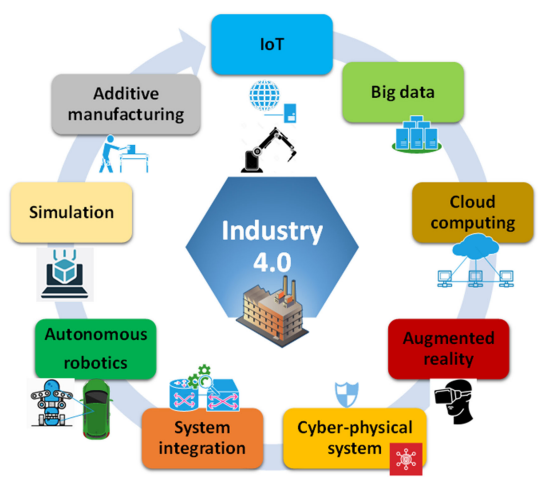
\includegraphics[width=0.7\linewidth]{figs/key-tech-industry-4.png}
    \caption{Key enabling technologies in Industry 4.0~\cite{Ahmed2022}}
    \label{fig:key-tech-industry-4}
\end{figure}
\FloatBarrier

With advancements in \ac{AI}, industrial processes can achieve unprecedented performance levels, often exceeding human capabilities. These \ac{AI}-driven systems enable robots to perform tasks that may be too hazardous, complex, or delicate for humans, such as handling dangerous materials or managing microscopic elements. Despite this extraordinary potential, it is important to recognize that current industrial robots are not as "smart" as humans in many contexts and, even though these robots are capable of performing highly skilled tasks, they frequently operate under strict, pre-programmed limits~\cite{Ahmed2022}.

Although Industry 4.0 has undoubtedly increased productivity, flexibility, and automation in industrial environments, it has also led to concerns regarding the diminishing role of human operators. This relentless push towards full automation has, in some cases, reduced human involvement in critical decision-making processes, leading to a more machine-centric production landscape~\cite{GOLOVIANKO2023102}.

\subsection{Industry 5.0: Reintegrating the Human Element}

Approximately a decade after the launch of Industry 4.0, the European Commission introduced the Industry 5.0 concept in response to new societal challenges~\cite{industry5}. The growing concerns about the exclusion of human operators in Industry 4.0 systems, coupled with the limitations of full automation, paved the way for this new industrial paradigm. Industry 5.0 seeks to reintroduce the human element into industrial ecosystems, emphasizing greater human involvement in manufacturing processes~\cite{Leng2022}.

The main goal consists on combining the strengths of humans and machines to achieve more sustainable, efficient, and human-centered production systems. This shift reflects the realization that, while machines excel at repetitive, dangerous, or complex tasks, humans provide irreplaceable creativity, adaptability, and problem-solving abilities~\cite{10577684}. Industry 5.0 aims to strike a balance between technological advancement and human-centric values, fostering environments where humans work alongside advanced technologies to achieve greater societal and environmental outcomes~\cite{GOLOVIANKO2023102}.


% While Industry 4.0 focused on pushing the limits of automation and data-driven production, Industry 5.0 reintroduces the importance of human collaboration. 
Recognizing that humans and machines each possess distinct strengths that can complement one another, the following key technological drivers of Industry 5.0 build upon the advancements of Industry 4.0~\cite{10577684}:
%  These drivers signify a shift towards greater human-machine collaboration, addressing the limitations of full automation while fostering more adaptive, intelligent, and human-centric industrial systems.

\begin{itemize}
    \item \textbf{Collaborative Robots (Cobots):} are engineered to ensure safe, collaborative operation alongside human workers, facilitating not only intuitive interactions but also fostering efforts that leverage the unique strengths of both humans and robots. Their integration is driven by the need to create systems that enable seamless, user-friendly \ac{HRC}, in full alignment with the guiding principles of Industry 5.0. This paradigm shift redefines traditional employment roles by emphasizing \ac{HRI}, with a focus on communication and coordination with robotic systems and advanced \ac{AI}.

    \item \textbf{Digital Twins:} represent a pivotal technological advancement in Industry 5.0. They provide visual models that enhance comprehension and facilitate the evaluation of goods, processes, and production systems. By allowing real-time monitoring and simulation, \ac{DT} help optimize manufacturing processes, bridging the gap between the virtual and physical worlds.

    \item \textbf{Human-Centric Automation:} Emphasis is placed on using technology to augment human capabilities rather than replace them, fostering a more inclusive, creative, and flexible manufacturing environment. This approach ensures that technology empowers human workers, enabling them to focus on tasks requiring intuition and creativity.

    \item \textbf{Advanced Human-Machine Interfaces:} The development of intuitive interfaces, by integrating technologies such as \ac{AR} and \ac{VR}, facilitates better communication between humans and machines. These interfaces allow for more natural interactions, improving understanding and efficiency in collaborative tasks.

    \item \textbf{Artificial Intelligence and Cognitive Computing:} These technologies continue to evolve, enabling robots and automation systems to work alongside humans in ways that enhance productivity without fully replacing them. \ac{AI} allows for more intuitive \ac{HMI}, where machines can understand and respond to human needs more effectively.

    \item \textbf{Sustainable and Resilient Manufacturing:} Industry 5.0 also focuses on sustainability and resilience, integrating environmental considerations into manufacturing processes. This includes optimizing resource usage and reducing waste, aligning technological advancement with ecological responsibility.
\end{itemize}

By integrating these key drivers, Industry 5.0 addresses the challenges identified in Industry 4.0, promoting harmonious collaboration between humans and machines. This synergy aims to enhance productivity while preserving the unique contributions of human workers, ultimately leading to more innovative, sustainable, and human-centered industrial practices.


% %%%%%%%%%%%%%%%%%%%%%%%%%%%%%%%%%%%%%%%%%%%%%%%%%%%%%%%%%%%%%%%%

% \section{Introduction to Industry 5.0} As a response to the increasing automation and the need for greater human involvement in manufacturing 
% processes, "Industry 5.0" seeks to reintroduce the human element into industrial ecosystems. Unlike Industry 4.0, which prioritized automation and 
% machine autonomy, Industry 5.0 emphasizes human-robot collaboration, where the strengths of humans and machines are combined to achieve more sustainable, 
% efficient, and human-centered production systems. This shift reflects the realization that while machines excel at repetitive, dangerous, or complex tasks,
% humans provide irreplaceable creativity, adaptability, and problem-solving abilities.

% Industry 5.0 seeks to strike a balance between technological advancement and human-centric values, fostering environments where humans work alongside 
% advanced technologies to achieve greater societal and environmental outcomes \cite{GOLOVIANKO2023102}.

\section{Human-Robot Collaboration}
%%%% estender um pouco mais e fazer ponte para collaboration scenarios / digital realities
\label{subsection:human-robot-collab}
% \input{chapters/stateofart/subsections/human-robot-collab}

The field of \ac{HRI} is dedicated to examining the interactions and coexistence of humans and robots in shared spaces, whose objective consists on enhancing these interactions by designing robots that are safe, effective and compatible for assisting and cooperating with humans in diverse roles, rather than replacing them \cite{Ogenyi2021}.
This involves developing robots that are, not only autonomous, but also capable of understanding and communicating with humans, as well as predicting
human-behavior and learning from human feedback. 

However, \ac{HRI} can be broken down into different forms of interaction, whose categorization is based on various factors that define how 
humans and robots share the workspace. This disctinction is represented in the Figure \ref{fig:collab} and can be broken down into \textbf{Coexistence}, \textbf{Cooperation} and \textbf{Collaboration} \cite{Jahanmahin2022}. 
Each one can be distinguished by the degree of interaction and task sharing between humans and robots:

% * TODO: i tried to edit it and center it, but it lost resolution. i will try to make it better
\begin{figure}[!htbp]
    % \centering
    % \hspace{-1.3cm}
    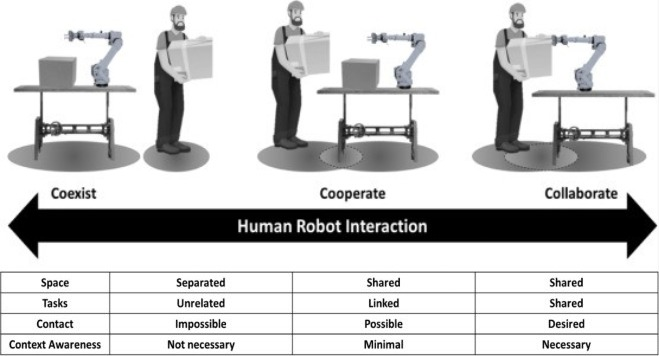
\includegraphics[width=\linewidth]{figs/table-figure-together.jpeg}
    \caption{Different levels of \ac{HRI}~\cite{Jahanmahin2022}} 
    \label{fig:collab}
\end{figure} 

\begin{itemize}
    \item \textbf{\ac{HRCx}}: In this form of interaction, humans and robots operate in the same environment but perform entirely independent tasks without interaction. The workspace is separated, there is no contact, and context awareness is unnecessary since the tasks are unrelated.
    Usually this interaction does not involve synchronized work or communication between the two parties. 

    \item \textbf{\ac{HRCp}}: Here, humans and robots share the workspace and work on linked tasks, towards a common goal. Advanced technologies such as sensors or machine vision may be used to detect and prevent collisions. Contact is possible, though not essential and actions are largely independent  with occasional coordinated efforts.

    \item \textbf{Human-Robot Collaboration (\ac{HRC})}: represents the most advanced and integrated form of \ac{HRI}. In \ac{HRC}, humans and robots not only share a common workspace but also actively collaborate on shared objectives. This collaboration can involve direct physical contact, such as the joint manipulation of objects, or non-physical interaction, including verbal communication, gestures, or pattern recognition.
    Within such environments, humans often handle tasks that require fine motor skills, decision-making, or creative problem-solving, while robots take on repetitive, strenuous, or hazardous activities, ensuring efficiency and safety. This synergy enhances productivity by leveraging the unique strengths of both humans and robots, creating a dynamic partnership where each complements the other’s capabilities.

\end{itemize}

In the bottom part of the Figure \ref{fig:collab} there is a table that further breaks down these distinctions, highlighting key factors like space, task relationship, possibility of contact, and the need for context awareness. This gradient from coexistence to collaboration shows the increasing complexity and interdependence in \ac{HRI}, as technology evolves to make robots more capable partners in industrial and service environments.

% explanation of the below figure
Below, the Figure \ref{fig:hrc-workstation} illustrates a \ac{HRC} workspace, showcasing the interaction between a human worker and a robot within a shared environment. The workspace is divided into distinct yet overlapping areas: the robot's work envelope and the human's work envelope. These areas reflect the respective tasks of each party, with the robot likely performing repetitive or automated tasks, such as material handling within the feeding system, while the human focuses on more intricate tasks requiring dexterity and decision-making.

The overlapping shared workspace demonstrates the core principle of \ac{HRC}, where humans and robots work together toward common goals, necessitating real-time coordination and communication. In this setup, advanced sensing technologies or machine vision are essential to ensure safety and prevent collisions, allowing both the human and robot to operate efficiently within close proximity.

This image underscores how robots, rather than replacing humans, complement human skills by taking on routine, physically demanding tasks, while humans contribute with their cognitive abilities. This partnership reflects the broader vision of Industry 5.0, where human creativity and robotic precision are combined to create adaptable, human-centered industrial processes, enhancing both efficiency and safety in collaborative environments.

\begin{figure}[!htbp]
    \centering
    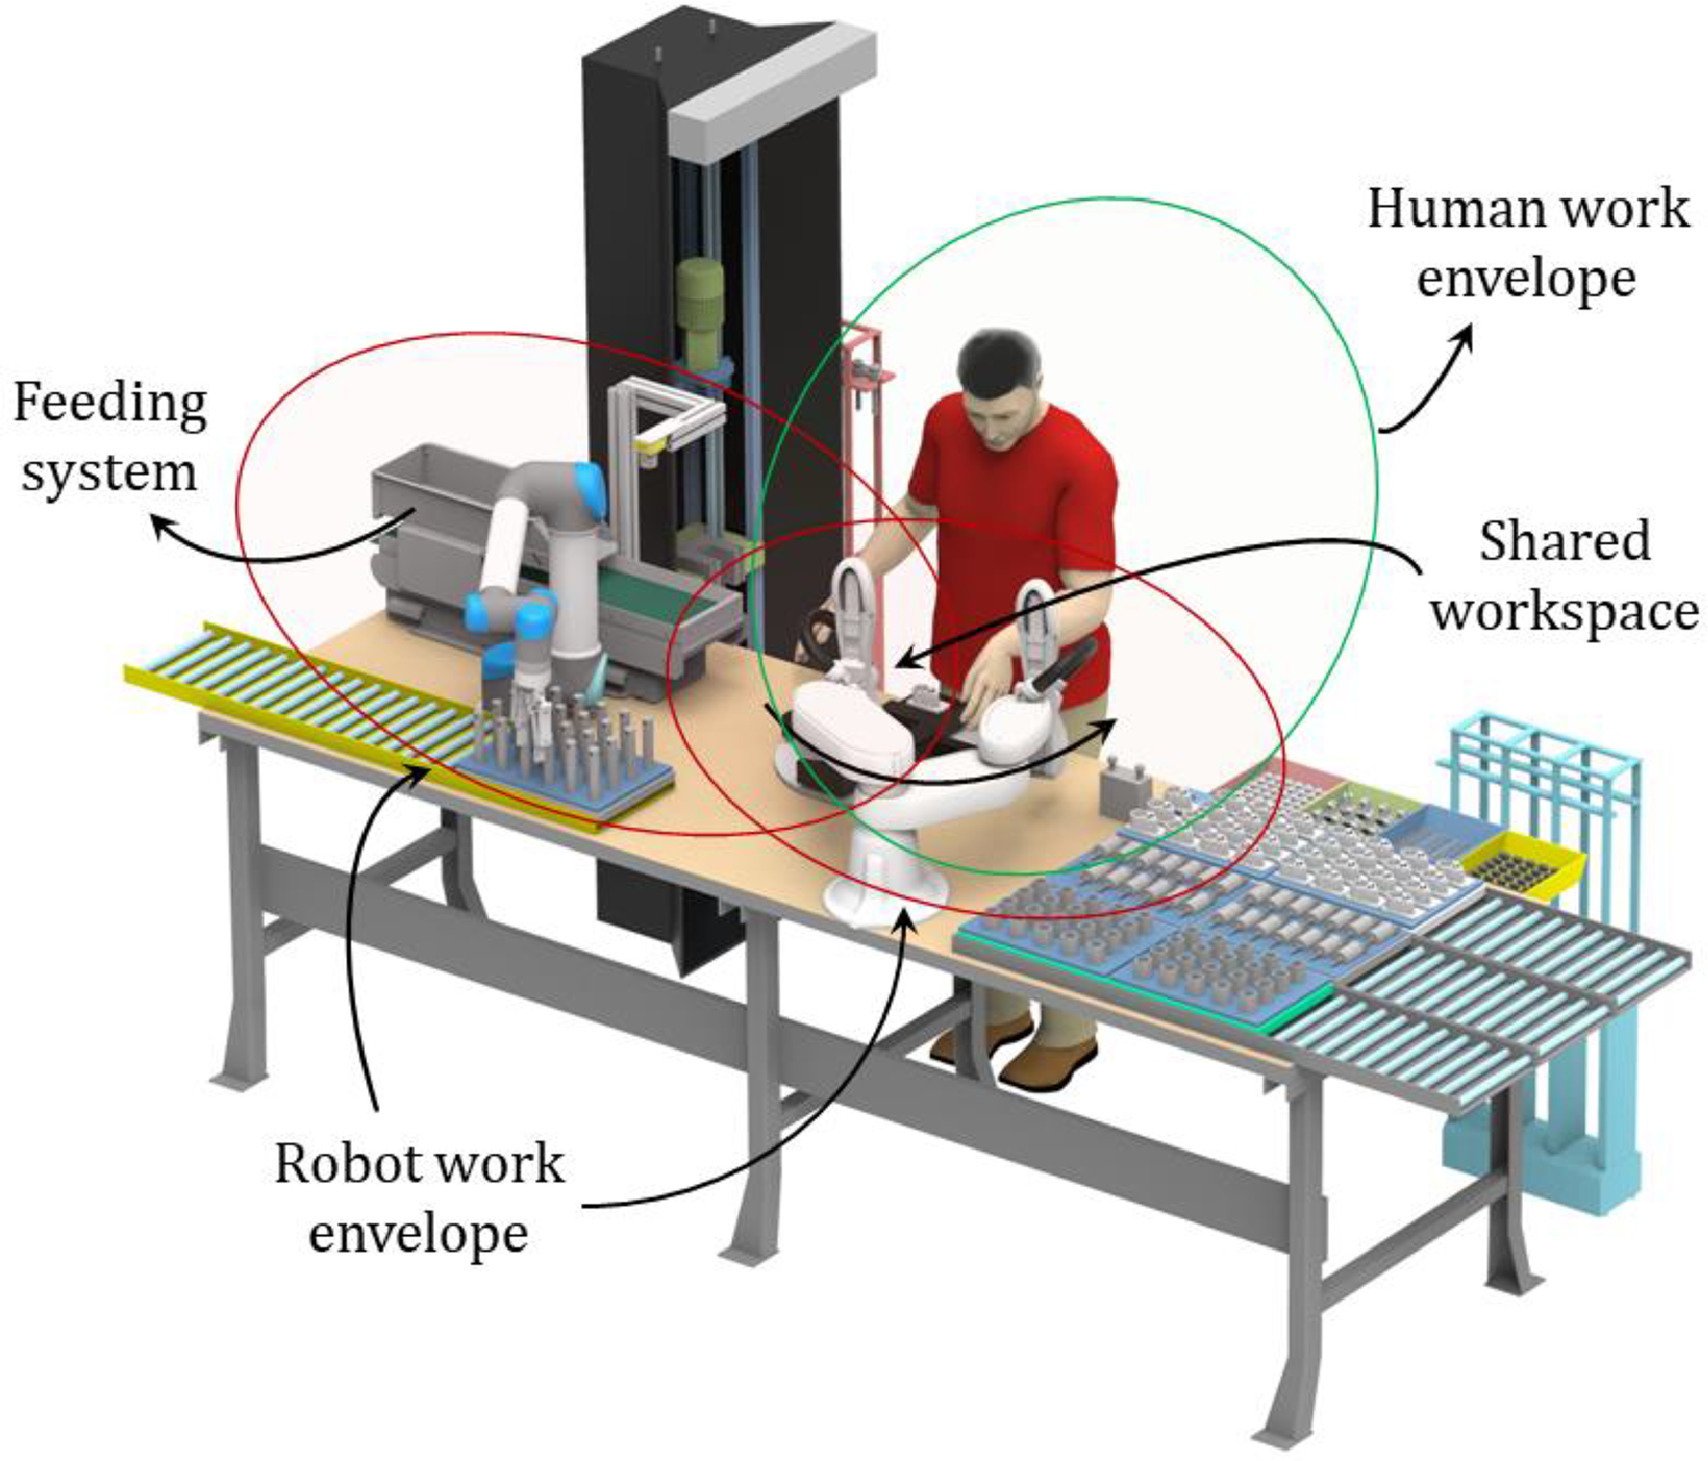
\includegraphics[width=0.7\linewidth]{figs/workspace-station-high-res-image.jpg}
    \caption{Workstation example enabling collaboration between human and robot while sharing the same physical space~\cite{MALIK2021102092}} 
    \label{fig:hrc-workstation}
\end{figure} 

%  link do artigo com a figura: https://www.sciencedirect.com/science/article/pii/S0736584520303021#fig0002
%  workspace-station-high-res-image - figura com alta resolução
%  workspace-station-full-image - figura full size

These new robots featuring intelligent sensing and vision systems, envisioned to integrate the production line, are called "cobots". 
They represent the alternative to full automation, since industry specialists have stated it is not possible to completely remove the 
human within the manufacturing environment \cite{Weiss2021}.

%% adicionar figura correta e dar label - verificar depois esta questao do estado da arte aqui

%%%%%%%%%%%%%%%%%%%%%%%% analise do artigo sobre cobots - Human–Robot Collaboration in Manufacturing Applications: A Review - 2019
%%%%%%%%%%%%%%%%%%%%%%%% ver melhor esta parte abaixo, organizar melhor e adicionar referencias bem, imagens e o que está a faltar
\section{Collaborative Robots (Cobots)} 

The concept of collaborative robots, or "cobots," was first introduced by J. Edward Colgate and Michael Pashkin in 1996 \cite{cobot-definition}, laying the foundation for practical applications in \ac{HRC}. Cobots are designed to physically interact with humans in shared workspaces, without the need for protective barriers typical in traditional robotic systems. This innovation paved the way for a new category of robots that excel in adaptability and flexibility, although effective use requires a deep understanding of their unique characteristics \cite{Aaltonen2019}.

\begin{figure}[!htbp]
    \centering
    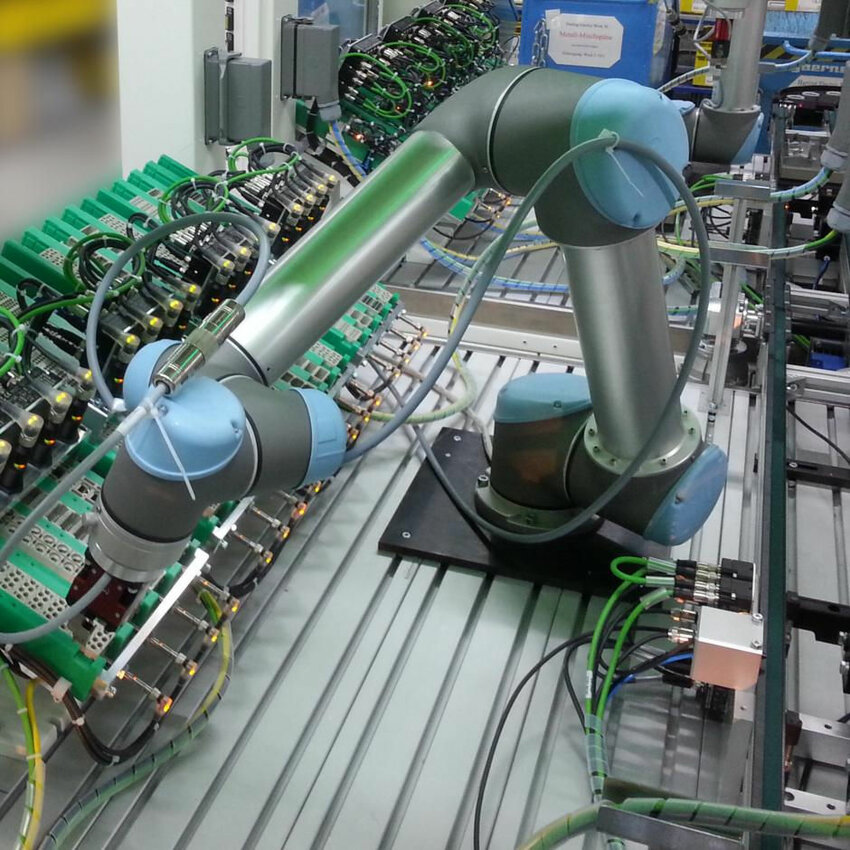
\includegraphics[width=0.55\linewidth]{figs/ur5-industry.png}
    \caption{UR5 light-weight cobot in industrial context \cite{Jeffrey-UR5}} 
    \label{fig:ur5}
\end{figure} 

The UR5, shown in Figure~\ref{fig:ur5}, represents a pivotal development in collaborative robotics, as it enabled quicker and more cost-effective adaptation of industrial layouts. Unlike traditional industrial robotic systems, which require extensive safety guarding and consequently reduce flexibility while increasing both costs and spatial demands, cobots present a solution tailored to the current market's demand for shorter lead times and mass customization, particularly for \ac{SMEs} \cite{barbazza2017agility}.

This cobots' emergence represents a paradigm shift in industrial automation, emphasizing \ac{HRC} over the traditional model of robotic isolation. These facilitate direct physical interaction between humans and machines while being designed for intuitive use, enabling even non-experts to reprogram them effortlessly \cite{7140065}. By leveraging the complementary strengths of human cognitive capabilities and robotic precision, cobots offer substantial productivity gains and reduced operational costs.

Cobots differentiate themselves from traditional industrial robots by prioritizing safety, ergonomics, and user accessibility. Unlike conventional robots that require extensive safety enclosures, cobots are equipped with advanced features such as force and torque sensors, vision systems, and anti-collision mechanisms. These capabilities enable them to operate safely in close proximity to humans without the need for restrictive barriers \cite{cobots-design}. The inherent design of cobots supports flexibility and ease of deployment, avoiding the high costs and complexity associated with retrofitting traditional robotic systems for similar functionality.

The adoption of cobots in industrial settings is driven by a combination of economic, operational, and health-related factors:
\begin{itemize}
    \item \textbf{Cost Efficiency:} Cobots can significantly reduce labor costs by performing repetitive tasks, thereby lowering direct unit production costs compared to traditional automation solutions \cite{cobot-2019collaborative}.
    \item \textbf{Enhanced Workplace Safety:} Their design minimizes occupational hazards, which leads to improved worker safety and health, addressing ergonomic challenges in manual labor.
    \item \textbf{Spatial Efficiency:} The compact and flexible nature of cobots allows them to be easily relocated and reconfigured within different production areas, optimizing factory space utilization \cite{cobots-implementation}.
\end{itemize}


These attributes are particularly beneficial in high-risk applications and industries that demand frequent changes in production layouts, such as electronics, automotive, and aerospace manufacturing.

When assessing the applicability of cobots versus traditional robots, several distinctions emerge. Cobots excel in tasks that require adaptability and human-like dexterity, such as assembly, placement, handling, and quality inspection. Their versatility and ease of integration make them suitable for low-volume, high-flexibility production environments, where agility is crucial. Despite their advantages, integrating cobots still encounters challenges for some use-cases. Lack of knowledge has a huge impact, for example regarding safety legislation, reference cases, and optimizing cobot potential applications in dynamic environments that require further research and development \cite{Aaltonen2019}.
Additionally, advancements in \ac{AI} and \ac{ML} could unlock new capabilities for cobots, enabling them to autonomously adapt to changing tasks and work conditions, thereby extending their utility beyond predefined, structured environments.

Moreover, \ac{MR} technologies are becoming increasingly pivotal in advancing cobot integration, offering immersive, real-time interfaces that enhance \ac{HRC}. By overlaying digital information onto the physical workspace, \ac{MR} facilitates better situational awareness and task execution for both operators and cobots. Coupled with \ac{DT} systems, \ac{MR} enables real-time monitoring and control of cobots in dynamic and remote settings, enhancing operational flexibility. Integrating \ac{MR} into cobot applications thus allows for more intuitive interactions, improved safety, and higher precision in collaborative environments. As part of Industry 5.0, these technologies collectively contribute to creating more responsive, human-centered manufacturing systems.

\section{Digital Realities} 
\ac{DR} encompass a wide spectrum of technologies that merge virtual elements with real-world environments to varying extents. In 1994, Milgram and Kishino introduced the Reality-Virtuality Continuum, a theoretical framework that characterizes the progression from a purely physical environment to a fully virtual one, as illustrated in Figure \ref{f:real-virtual-continuum} \cite{milgram1994}.
This continuum is divided into four principal stages: Reality, \ac{AR}, \ac{AV}, and \ac{VR}.

\begin{figure}[h]
    \centering
    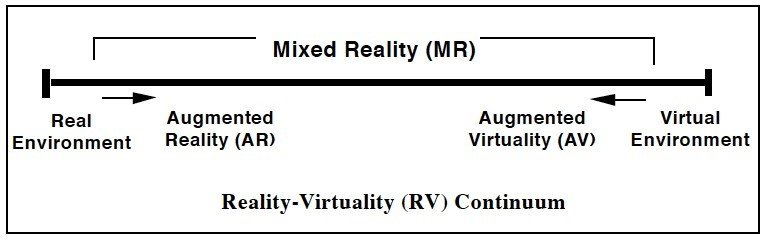
\includegraphics[width=0.9\linewidth]{figs/vr-continuum.png}
    \caption{Reality-Virtuality Continuum~\cite{milgram1994}}
    \label{f:real-virtual-continuum}
\end{figure}

In this continuum, Reality represents the perception of an unaltered physical environment, devoid of any virtual modifications. As we progress along the continuum towards the virtual side, different digital realities offer increasingly immersive experiences by blending or replacing real-world content with virtual elements.

\subsection{Augmented Reality}
    \ac{AR} enhances a user's interaction with their physical environment by overlaying dynamic digital content, such as 3D objects, information layers, or media, onto the real world \cite{liu2022digitaltwin}. The main goal of \ac{AR} is to seamlessly integrate virtual objects with the user's surrounding physical context, facilitating real-time interaction between the virtual and physical realms allowing users to experience both virtual and real entities as coexisting within the same space, generating a cohesive and interactive environment \cite{Azuma1997}.
    
    Figure \ref{f:ar-example} \footnote{\url{https://www.cad-schroer.de/news-events/artikel/mixed-reality-augmented-reality-virtual-reality-definition-und-uebersicht/}, Acessed: 2024-10-19} provides a clear representation of \ac{AR} being employed in an industrial maintenance scenario. The user views real-time digital overlays on a physical machine, providing essential information such as the machine’s current status and highlighting critical components for maintenance or repair. This visual guidance significantly enhances the user’s understanding of tasks by seamlessly blending virtual instructions with the real environment, thereby improving efficiency and reducing the potential for human error.

    \begin{figure}[!htpb]
        \centering
        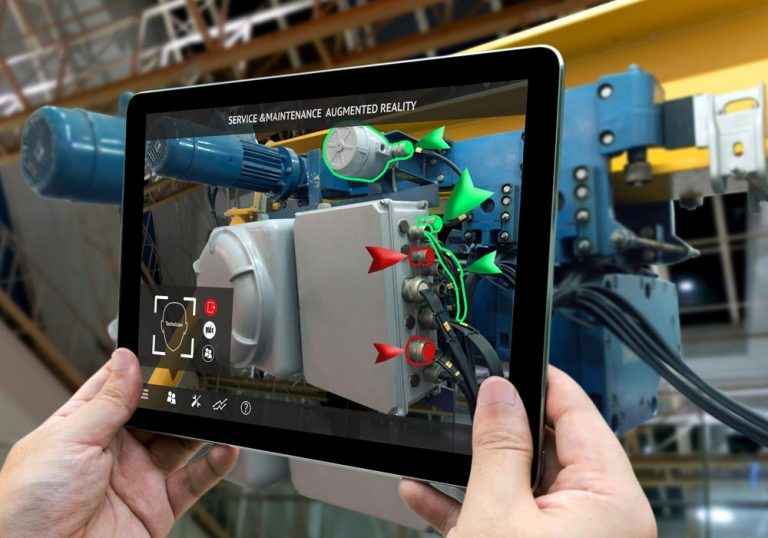
\includegraphics[width=0.6\linewidth]{figs/ar-example.jpg}
        \caption{Augmented Reality application of industry overlayed information in order to assist the operator}
        \label{f:ar-example}
    \end{figure}

    Achieving this level of integration requires accurate spatial registration, a process that ensures that virtual elements are properly aligned with real-world objects in both location and scale. The spatial coherence between the two realities is critical for creating an effective \ac{AR} experience, where virtual objects respond to changes in the environment and user interaction in real-time. 

    Various \ac{AR} devices are employed to deliver these experiences, including \ac{AR}-\ac{HMD}, tablets, \ac{HHD}, projectors, and see-through \ac{VR} headsets with built-in cameras. Each device offers different degrees of environmental awareness and interaction capabilities, such as hand tracking and holographic projection. 
    % These technologies have transformed numerous industries, offering new possibilities in fields ranging from manufacturing and design to healthcare and entertainment.

    * TODO: add more references to the above 2 paragraphs

\subsection{Virtual Reality}
    
    Within the Reality-Virtuality Continuum proposed by Milgram and Kishino, \ac{VR} occupies the extreme end of the spectrum, representing a complete substitution of a user’s perception of the physical world with a fully immersive synthetic environment. In this state, the user is entirely isolated from their real surroundings, perceiving only the artificially constructed virtual environment, typically presented through a range of immersive devices such as \ac{HMD} \cite{milgram1994}. Figure~\ref{f:real-virtual-continuum} \footnote{\url{https://en.wikipedia.org/wiki/Immersion_\%28
    virtual_reality\%29\#/media/File:Reality_check_ESA384313.jpg}} illustrates this immersive experience where the user interacts with a virtual environment through \ac{VR} equipment.

    \begin{figure}[h]
        \centering
        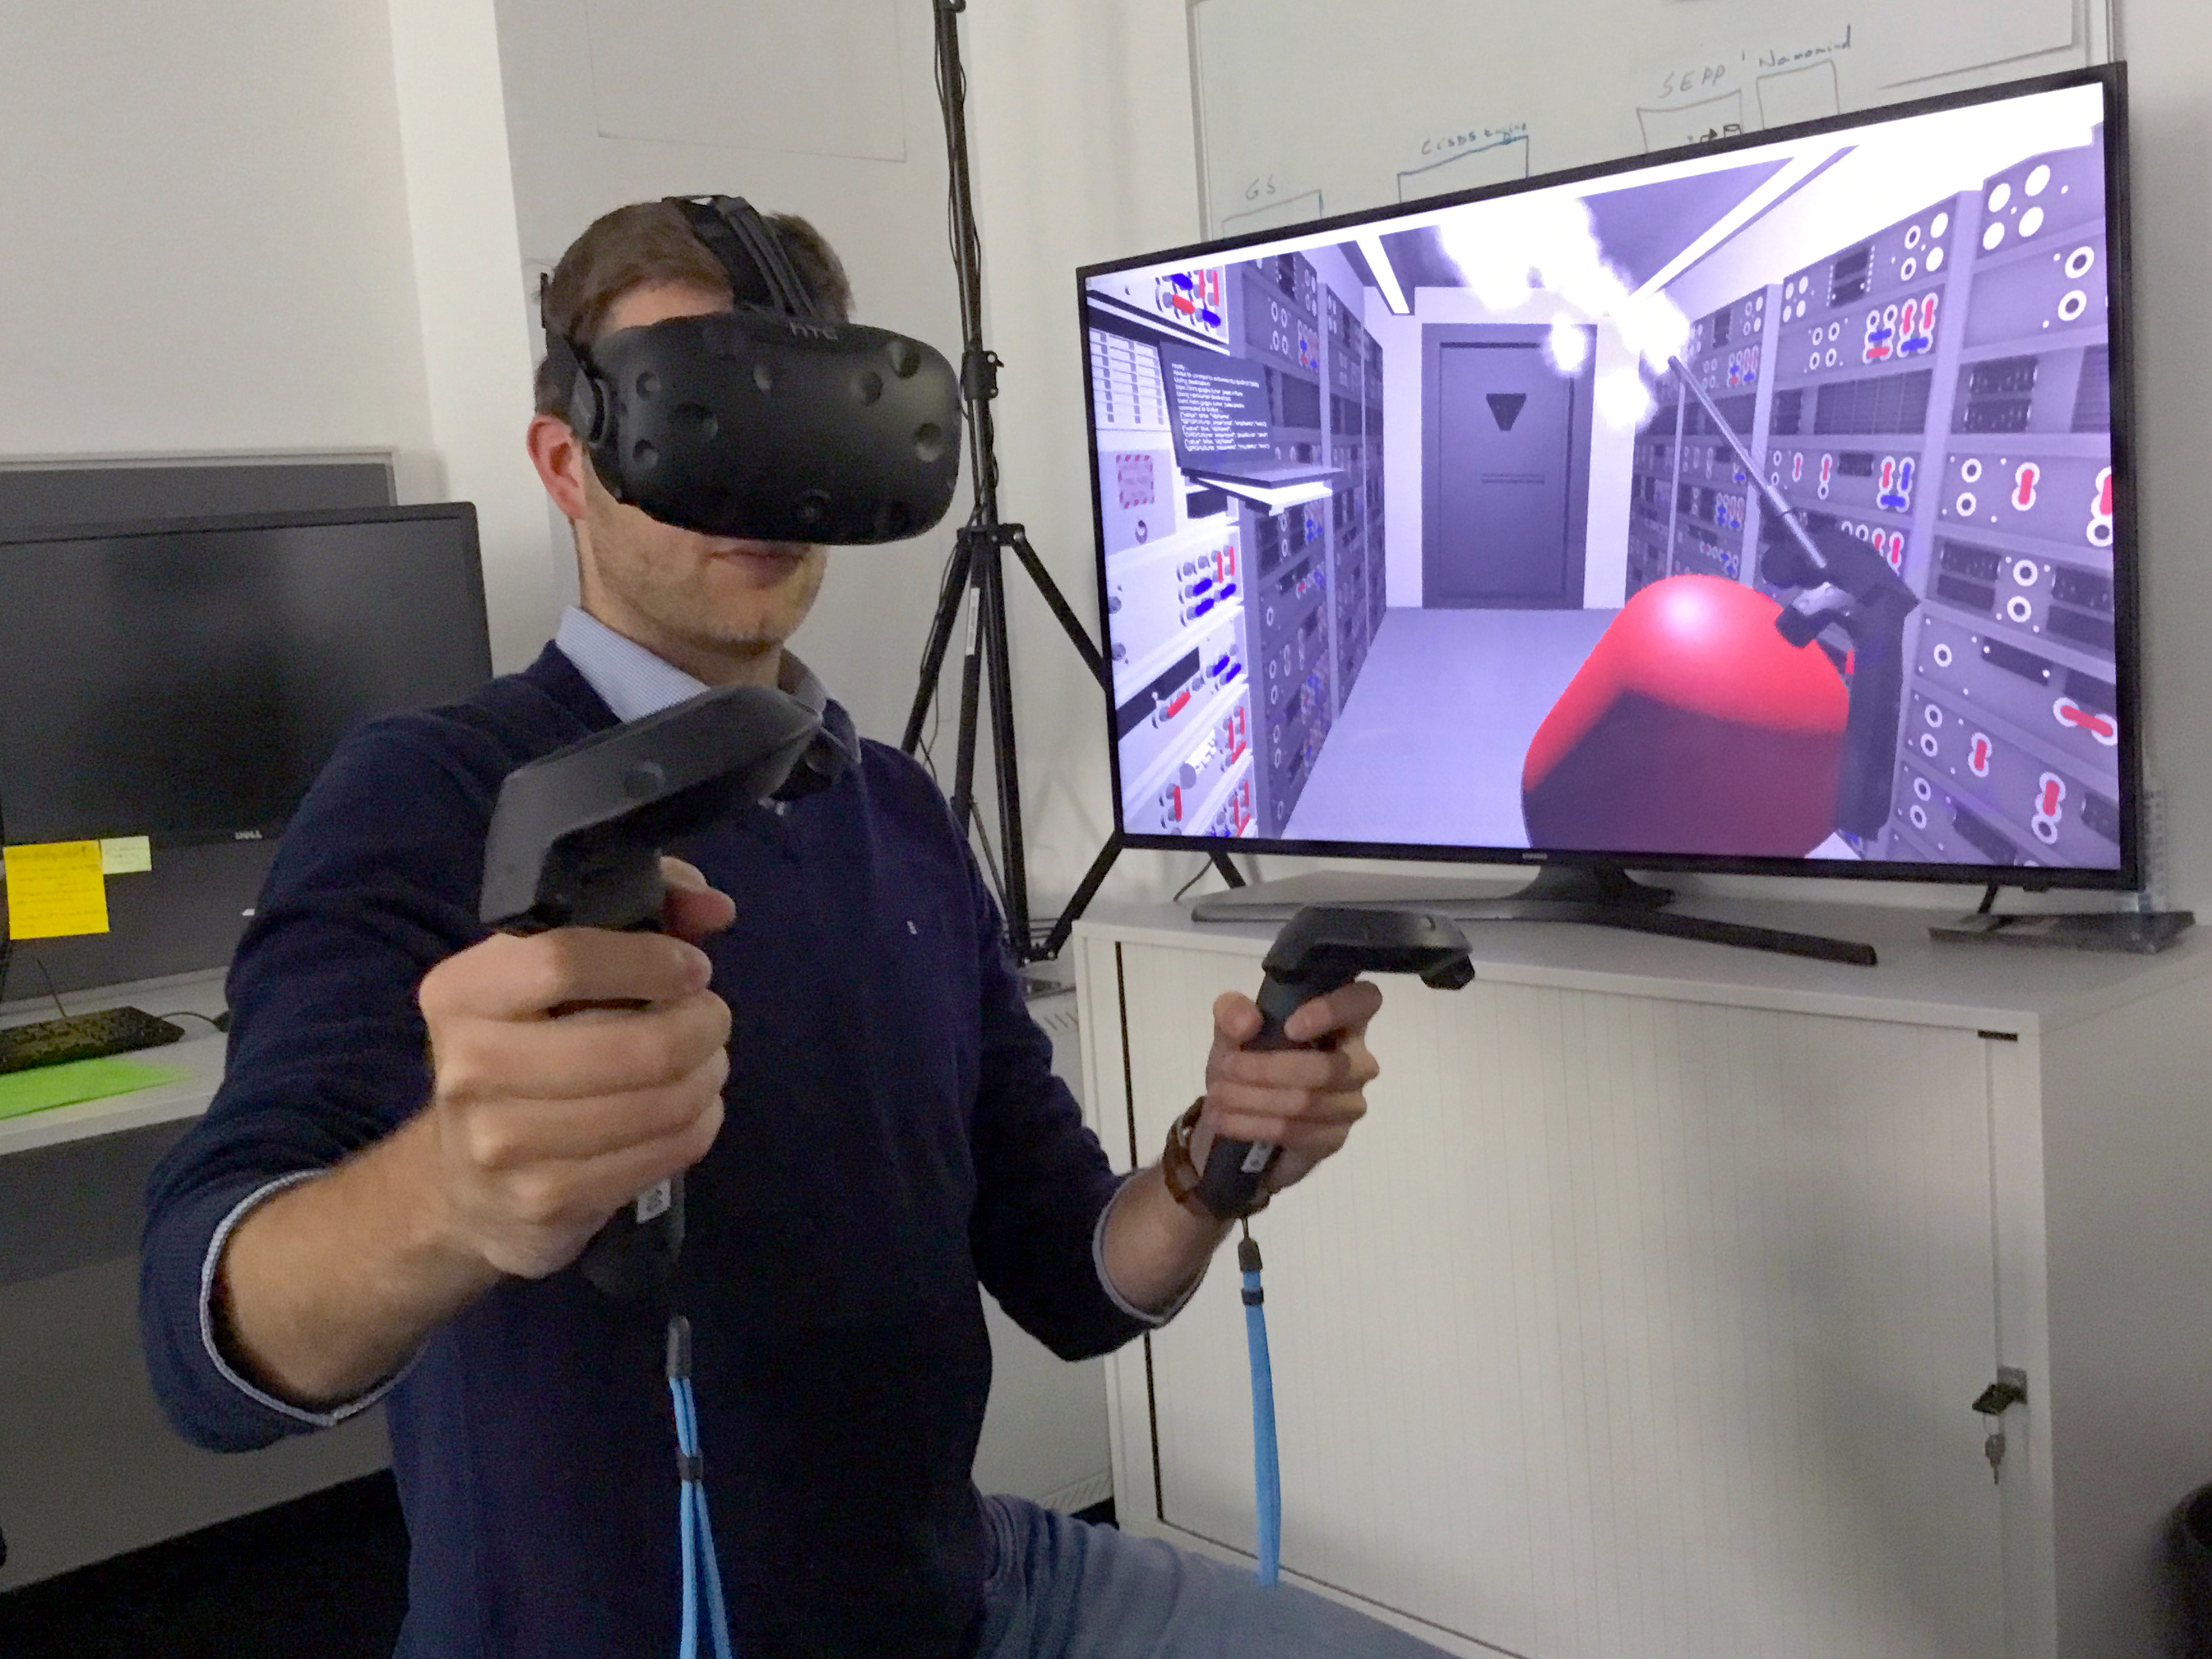
\includegraphics[width=0.6\linewidth]{figs/Reality_check_ESA384313.jpg}
        \caption{User immersed in a virtual environment using a VR headset, demonstrating complete isolation from the physical world.}
        \label{f:real-virtual-continuum}
    \end{figure}

    Modern \ac{VR} systems achieve this full immersion by leveraging advanced \ac{HMD}, which present stereoscopic images directly to the user’s eyes through built-in displays or projection systems. These devices often incorporate additional features like head tracking, enabling the user’s head movements to influence their viewpoint in the virtual environment, further enhancing the sense of immersion and presence \cite{whatismixedreality}. Some systems also include positional tracking through external sensors or inside-out tracking via integrated cameras, allowing users to physically navigate virtual spaces, augmenting both interaction fidelity and spatial awareness.

    \ac{VR} is particularly effective in applications that require the user to be completely enveloped in an artificial environment, thus enabling the simulation of real-world scenarios, historical reconstructions, or entirely imaginative worlds. This sense of "presence," wherein users perceive the virtual environment as real, is fundamental to \ac{VR}'s efficacy across various domains, including gaming, education, training, and simulation. Additionally, \ac{VR}'s potential to create deeply immersive and isolated experiences makes it especially valuable in fields like remote collaboration, where users can interact with simulated environments or models that are otherwise inaccessible \cite{8712803}.

    * TODO: add more references here  

    % \begin{figure}[h]
    %     \centering
    %     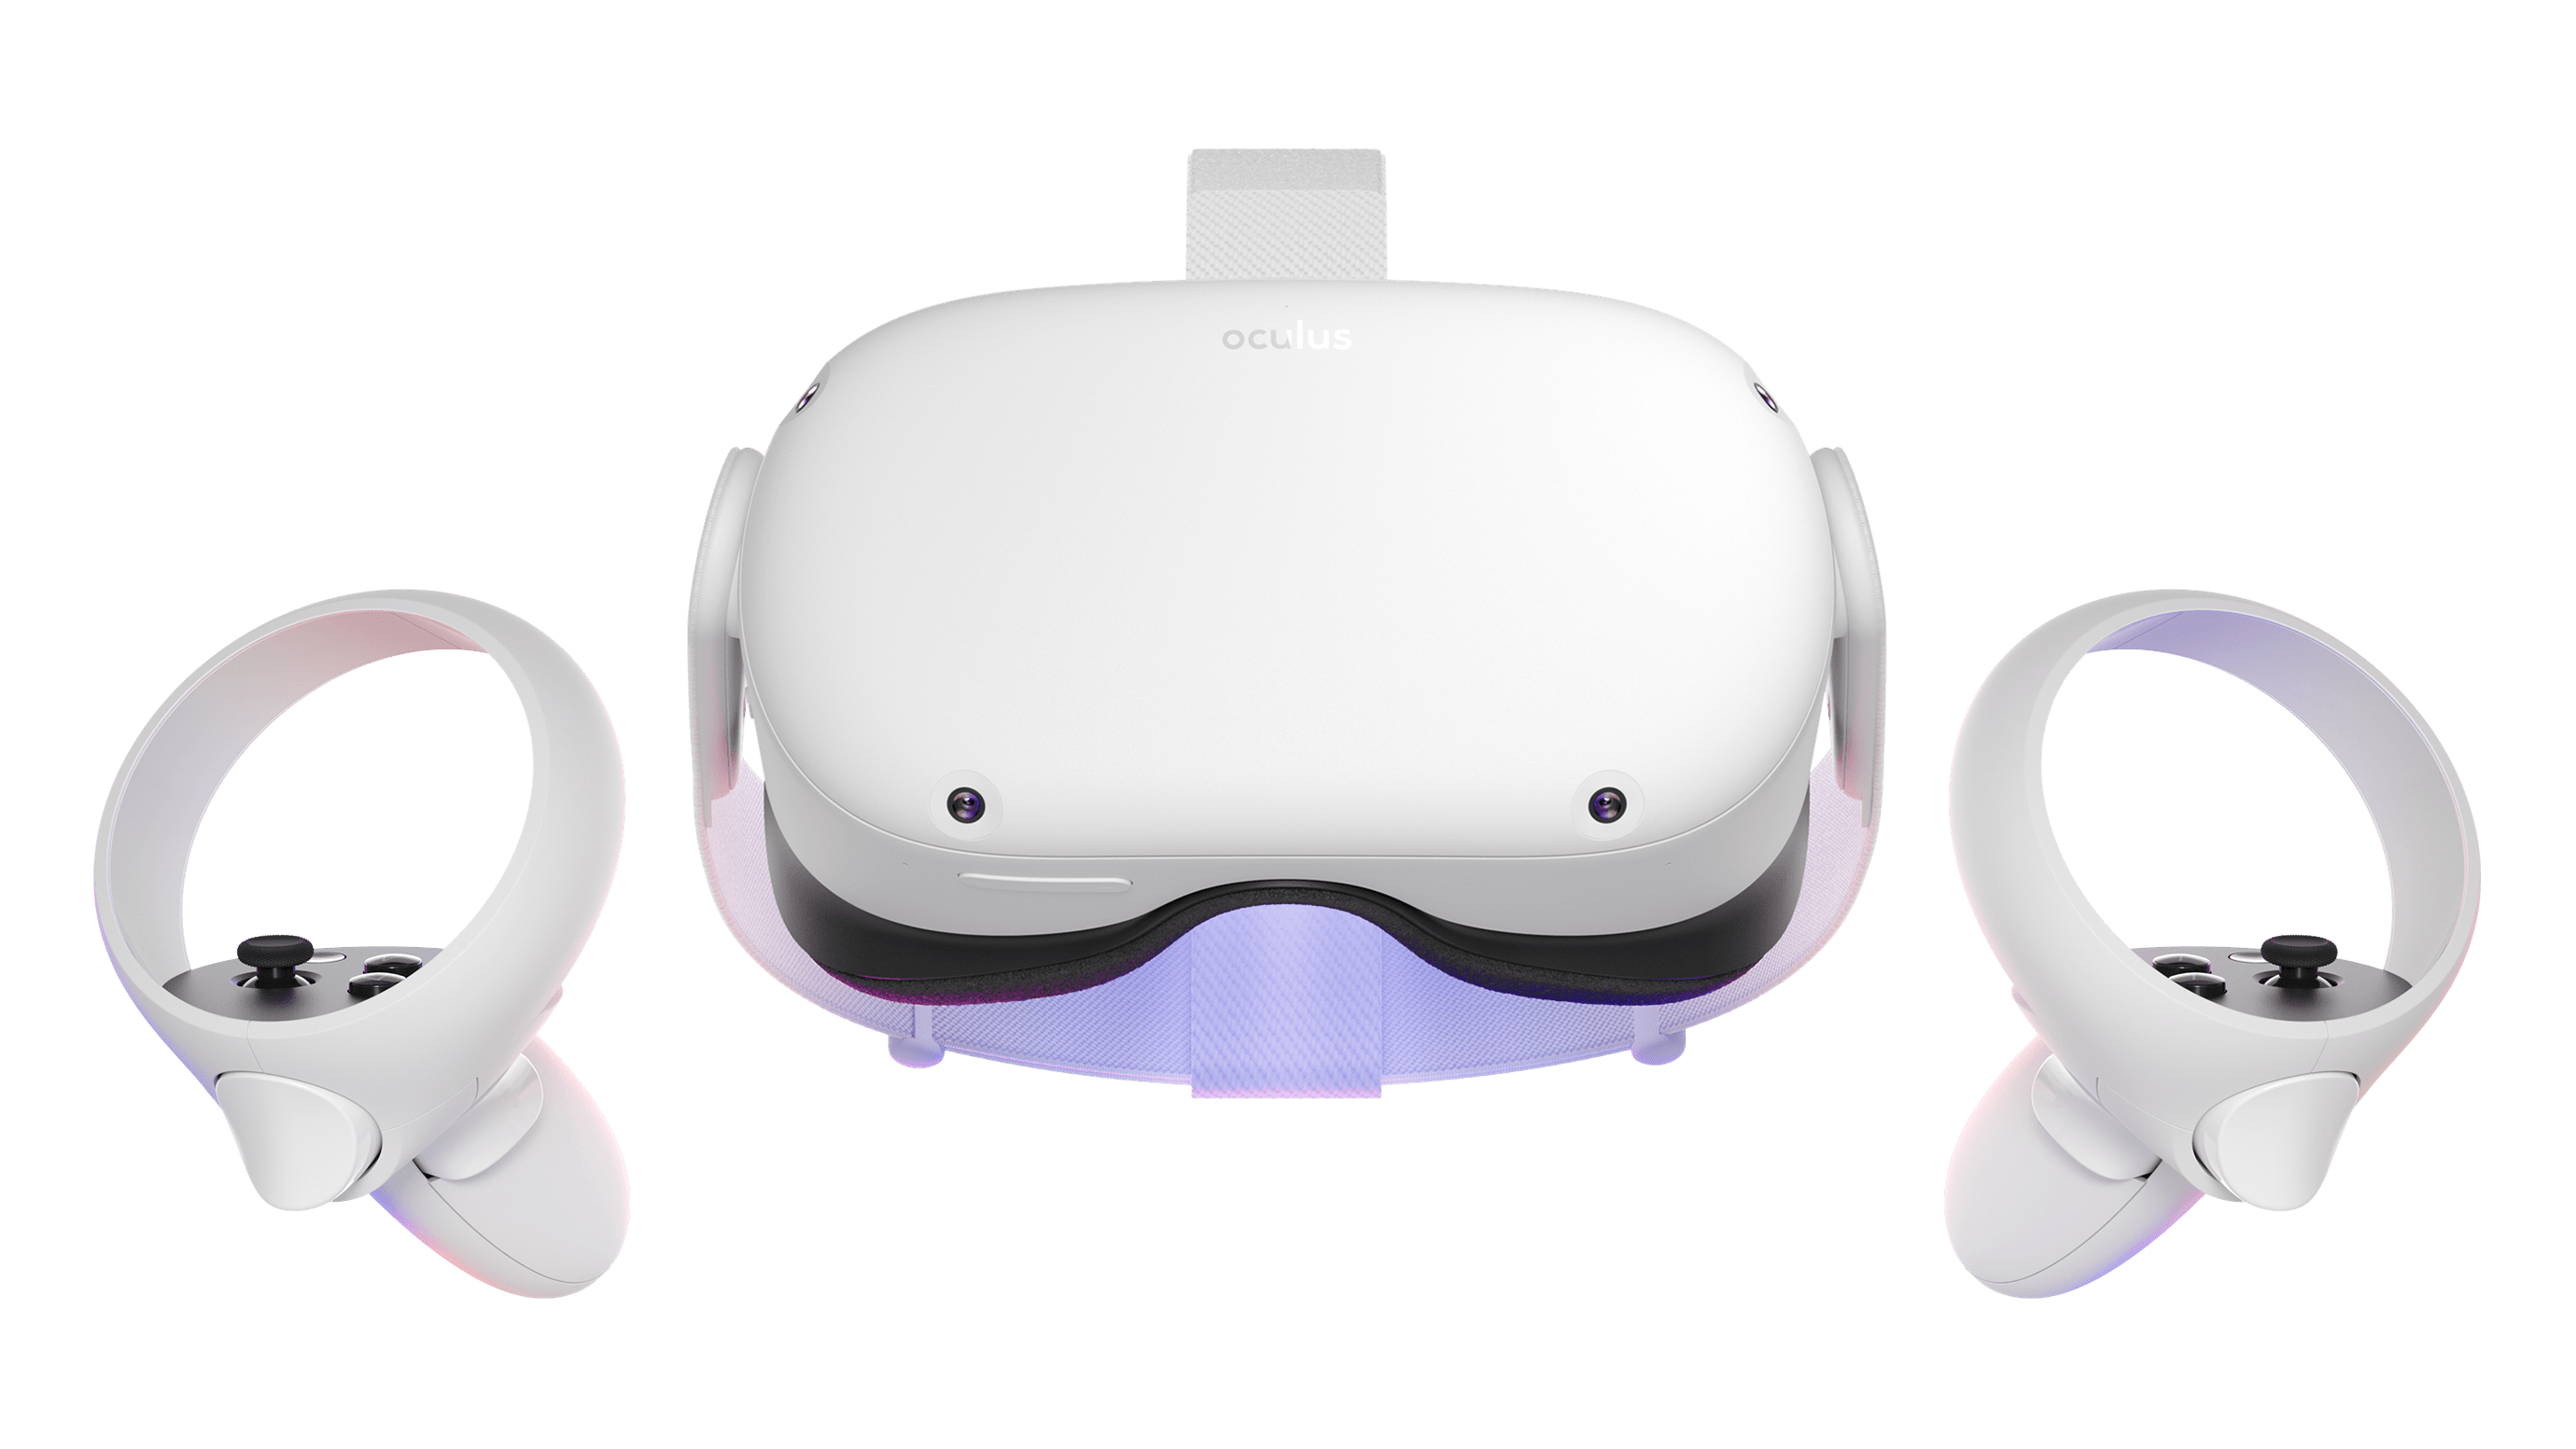
\includegraphics[width=0.6\linewidth]{figs/oculus-2-vr.png}
    %     \caption{Oculus Quest headset}
    %     \label{f:quest-2-vr}
    % \end{figure}

\subsection{Mixed Reality}
\label{subsection:digital-realities}
   
    \ac{MR} continues to elude a universally accepted definition, with interpretations diverging significantly across academic and industrial domains. According to the Milgram and Kishino Reality-Virtuality Continuum, depicted in Figure \ref{f:real-virtual-continuum}, \ac{MR} occupies a transitional space between \ac{AR} and \ac{AV}, bridging the two concepts \cite{milgram1994}. Expanding on this, Microsoft’s \ac{MR} spectrum~\footnote{\url{https://learn.microsoft.com/en-us/windows/mixed-reality/discover/mixed-reality}} defines \ac{MR} as spanning a range of technologies, from \ac{AR} (where physical reality predominates, augmented with digital overlays) to \ac{AV} (where the virtual environment dominates, supplemented by real-world data). 

    * TODO: ADD REFERENCES IN BELOW TEXT
    In \ac{MR} environments, digital and physical elements coexist and interact in real time, creating a dynamic interface where virtual and physical worlds seamlessly blend. This enables immersive, bi-directional interaction, where users engage with both digital objects and real-world elements, facilitating fluid communication between virtual entities and the physical environment. This integration enhances the user experience by enabling virtual objects to influence, and be influenced by, real-world contexts in a highly interactive manner, enabling new forms of collaboration, visualization, and interaction.

    The inherent complexity of \ac{MR} arises from the challenge of ensuring a natural and intuitive integration of digital and physical elements. This requires advanced environmental sensing, real-time data fusion, and contextual understanding to deliver interactions that appear natural to the user. 

    Despite considerable advancements, the definition of \ac{MR} remains contested. Speicher et al. (2019) identified six competing notions of \ac{MR} across both scholarly literature and industry practice, underscoring the fragmentation in its interpretation. Some experts argue that \ac{MR} represents an enhanced form of \ac{AR}, where users are not merely passive observers but active participants interacting with a responsive augmented space. In this interpretation, \ac{MR} is seen as a "stronger" form of \ac{AR}, exemplified by technologies such as Microsoft's HoloLens, where users can manipulate virtual elements within their physical environment \cite{whatismixedreality}.

    Other perspectives view \ac{MR} as a convergence of \ac{AR} and \ac{VR}, where the boundary between the real and virtual worlds is fluid and adaptable, creating immersive, hybrid experiences. For example, the widely known game Pokémon Go is sometimes cited as an \ac{MR} application, where a \ac{VR}-based digital environment enables users to interact with augmented digital elements such as Pokémons, overlaid onto the physical world \cite{whatismixedreality}.

    However, the definition most relevant to this project's development emphasizes \ac{MR} as a powerful medium for collaboration, enabling users to interact across different realities—whether physical, augmented, or virtual. In this context, \ac{MR} facilitates shared experiences between users located in distinct environments. For example, a physical space visualized by an on-site \ac{AR} user can be simultaneously recreated and experienced by a remote \ac{VR} user, allowing real-time collaborative interactions between participants situated in different realities. This capacity for cross-reality collaboration enhances both the user’s understanding of the workspace and the efficiency of the collaboration process.

    An example of this collaborative interaction is depicted in Figure \ref{fig:mr-collab-example}, where a trainer (remote) and trainee (on-site) engage in a task that bridges physical and virtual worlds. In this scenario, the trainee uses \ac{VR} technology to operate within a virtual environment, while the trainer remotely observes and provides guidance. Through this setup, the trainer can not only visualize the trainee's actions but also trigger events or scenarios via a dedicated interface, enhancing the learning experience. This type of interaction exemplifies the capabilities of remote training, where an expert can guide an on-site operator using real-time augmented indications displayed on \ac{AR} glasses or tablets. By providing direct visual and auditory feedback, the remote trainer assists in troubleshooting, guiding the trainee through complex tasks or maintenance operations. This form of collaboration allows geographically distant participants to work synchronously in a highly interactive environment, increasing both efficiency and accuracy in training processes \cite{Mayer2023}.
  
    % Mayer2023 referencia da figura
    \begin{figure}[h]
        \centering
        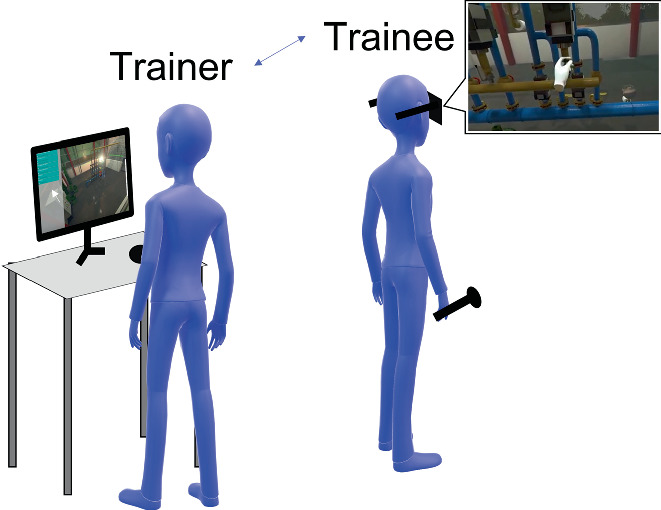
\includegraphics[width=0.7\linewidth]{figs/mr-example-collab.png}
        \caption{Collaborative setup for training in industrial scenarios using \ac{MR} \cite{Mayer2023}}
        \label{fig:mr-collab-example}
    \end{figure}

    *TODO: Verify this part a bit better - clarify the distinction between the referenced collaboration scenario and the collaboration of this dissertation, can I say that the remote user sees is immersed into an VR environment that the on-site also sees? because the on-site member sees it via AR and not only VR? 
    
    Although this example highlights the collaborative potential of \ac{MR}, it slightly differs from the ideal collaboration model developed in this project. Here, the focus is on enabling an \textbf{on-site} user to interact with the real world through \ac{AR}—visualizing real-time data overlaid onto their physical environment—while the \textbf{remote} user experiences the same \ac{VR} environment. This configuration allows the remote user to be fully immersed in a virtual reconstruction of the on-site environment, with the ability to monitor and collaborate with the on-site user in real-time. The goal is not only to enhance communication but to enable mutual interaction with a shared digital-physical environment, fostering more precise decision-making, particularly in complex, dynamic tasks. This setup, more reflective of the full potential of \ac{MR}, aligns closely with Industry 5.0’s vision of combining human expertise and advanced technology for seamless collaboration between humans and machines across different realities.

\section{Digital Twins}
\label{sec:dt}
Another relevant concept are \ac{DT}, which consist on sophisticated digital replicas of physical entities, allowing for the simulation, analysis, and control of systems within a digital framework. These digital counterparts have emerged as pivotal technologies in a variety of domains, particularly in enhancing \ac{HRC}, as they offer real-time, interactive environments that mirror physical systems. The ability to replicate physical entities with high fidelity enables improved decision-making, operational efficiency, and flexibility across a wide range of industrial applications.
*TODO: add a reference above

This \ac{DT} concept was first introduced by NASA in the 1980s as part of its spacecraft monitoring systems, where virtual models were employed to replicate the conditions and behavior of spacecraft during missions. Over the past decades, advances in \ac{IoT}, sensor technology, and computational power have significantly improved the capabilities of \ac{DT}, moving beyond their original use case. Modern systems leverage real-time sensor data and advanced simulation techniques to enhance the accuracy and reliability of digital models, enabling more sophisticated predictions, real-time analytics, and simulations of complex systems \cite{liu2022digitaltwin}.

In current manufacturing and industry scenarios, \ac{DT} play a transformative role, particularly in smart manufacturing systems, where they enable detailed examination and prediction of the behavior of physical systems. This capability allows companies to optimize operations, reduce downtime, and improve overall system efficiency. Furthermore, in \ac{HRC}, \ac{DT} facilitate safer and more productive work environments by dynamically adjusting robotic movements and operations to better align with human needs, thereby enhancing ergonomic interactions and mitigating safety risks \cite{8477101}.

A prominent real-world implementation of this technology is seen in Singapore's Smart Nation Initiative, where the Land Transport Authority employs a \ac{DT} to simulate and evaluate potential policy decisions before their implementation. This application exemplifies the wide-ranging potential of \ac{DT} to support decision-making processes in urban planning, infrastructure management, and beyond \cite{isprs-archives-XLII-4-W7-37-2017}. As these technologies evolve, their applications in both academic research and industrial practice are rapidly expanding.

The academic landscape surrounding \ac{DT} has seen extensive research exploring their versatility and potential, having been applied to a broad spectrum of areas, illustrating the profound impact of \ac{DT} on enhancing system efficiency, predictive maintenance, and overall operational performance \cite{8361285, TAO2018169, isprs-archives-XLII-4-W7-37-2017, 10.1007/978-3-030-23162-0_19, 6296978}.
*TODO: usar uma destas referencias para pôr no paragrafo introdutorio sobre os DT.

Despite the growing prominence of \ac{DT}, there is still no universally accepted formal definition of the concept. However, most scholars and industry experts concur that a \ac{DT} is a type of \ac{CPS} consisting of three fundamental components: a physical system, a virtual model, and bidirectional communication between these two models \cite{TaoFei, 8477101, ROSEN2015567}.
This interaction is fundamental to the operation of true \ac{DT}, allowing for a continuous feedback loop where changes in the physical world can inform the virtual model, and, in turn, decisions or optimizations made in the digital realm can directly influence the physical system.

In contrast to true \ac{DT}, some critics argue that many commercially available implementations, such as those provided by companies like Siemens, represent "digital shadows" rather than full \ac{DT}. The distinction lies in the capability for bidirectional communication. In many digital shadow systems, changes in the physical system are reflected in the virtual model, but there is no capacity for the virtual model to directly control or alter the physical system. This one-way communication limits the interactive and predictive capabilities that define a true DT \cite{CIMINO2019103130}.

To illustrate the distinction, Figure \ref{f:dt-structure} presents a reference model of a \ac{DT}, showcasing the bidirectional flow of information between physical and digital entities. This structure is essential for enabling real-time interaction and feedback, core characteristics that  differentiate \ac{DT} from digital shadows. True \ac{DT} must facilitate a continuous, reciprocal exchange of data between physical and virtual domains, allowing the virtual model to reflect and affect the physical system \cite{dt_model}.

\begin{figure}[!htpb]
    \centering
    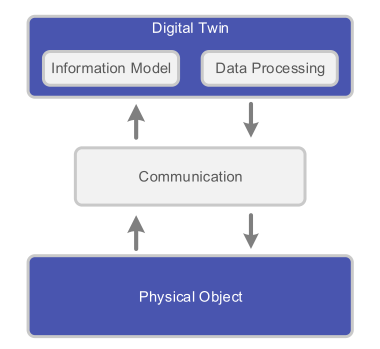
\includegraphics[width=0.55\linewidth]{figs/dt_reference_model.png}
    \caption{A Digital Twin reference model, emphasizing the importance of bidirectional communication between the physical object and its digital counterpart~\cite{dt_model}}
    \label{f:dt-structure}
\end{figure}

Bidirectional communication's importance in \ac{DT} is further emphasized by Liu et al.~\cite{liu2022state}, who argue that “a true DT must include bidirectional communication instead of having a virtual model that only updates according to a physical system.” This distinction between the types of communication and interaction is critical, as it defines the extent to which a \ac{DT} can be leveraged for control, simulation, and predictive purposes.

Table \ref{tab:levels_of_control} outlines different interaction levels within \ac{DT} systems, ranging from no interaction, where the physical and virtual systems are disconnected, to unidirectional data flow, where data is transferred from the physical to the virtual model, and culminating in bidirectional communication. The latter represents a fully functional \ac{DT}, where continuous exchange of data allows the virtual model to influence and control the physical system, achieving real-time synchronization and interaction.

% Table \ref{tab:levels_of_control} illustrates interaction levels present in \ac{DT} systems, from no interaction, to unidirectional data flow, and ultimately to bidirectional communication, the latest defining a fully functional \ac{DT}.

\begin{table}[!htpb]
    \centering
    \caption{Levels of Interaction in a Digital Twin system between the physical model and its digital counterpart, adapted from \cite{liu2022state}}
    \label{tab:levels_of_control}
    \begin{tabular}{@{}l>{\raggedright\arraybackslash}p{10cm}@{}}
    \toprule
    Level of Interaction & Description \\ 
    \midrule
    No interaction & Virtual model and physical system are not connected through a network. The virtual model only simulates and models a physical 
    system without any real-time updates. \\ \hline
    Unidirectional & The physical system feeds sensor data to the virtual model through a network. The virtual model utilizes data to update the 
    current state and predict future states. \\ \hline
    Bidirectional & Both the physical system and the virtual model can send data to each other. The virtual model updates using physical data while 
    the physical system can be controlled through data sent by the virtual model. \\ 
    \bottomrule
    \end{tabular}
\end{table}


\section{Human-Robot Collaboration in Industrial Applications}
\label{sec:hrc-in-industry}
Following the detailed exploration of \ac{DT} and \ac{MR}, this section discusses how these technologies integrate into \ac{HRC}, demonstrating significant improvements in interaction, safety and efficacy in practical examples from industry solutions with specific emphasis on remote collaboration.

The articles cited below often reference \ac{AR}, however, it is important to note that in many cases, the features described under \ac{AR} align more closely with the concept of \ac{MR} as a medium for collaboration, as explained in \ref{subsection:digital-realities}. This distinction is crucial, as the developed system is more aligned with \ac{MR}’s capability to further facilitate shared virtual and physical environments, enhancing interaction and collaborative processes across industrial applications.

\subsection{Enhancing Human-Robot Collaboration through Augmented Reality and Digital Twin Implementation}
 
Chu et al.~\cite{CHU2023313} reviewed various studies on integrating \ac{AR} with \ac{DT} to improve \ac{HRC} using visual and haptic feedback interfaces. Their work emphasizes the value of \ac{AR} in enhancing human-robot communication by providing both egocentric (shared remote views) and exocentric (spatial visualization of the robot relative to the workspace) perspectives, thereby improving spatial awareness and interaction quality. 

Green et al.~\cite{doi:10.5772/5664} further highlight that multimodal \ac{AR} interfaces—incorporating visual, haptic, and acoustic cues—can significantly enhance \ac{HRC}. Multimodal approaches help overcome challenges like limited \ac{FOV} in \ac{HMD}, making the interaction more intuitive. For instance, audio-tactile feedback is particularly beneficial for individuals with visual impairments, providing alternative sensory channels without compromising performance. Visual \ac{AR} cues, implemented through \ac{HMD}, help users navigate complex environments by overlaying relevant information, thus enhancing navigation without impeding robotic movement.

Lasota et al.~\cite{doi:10.1177/0018720814565188} conducted experiments to evaluate the impact of human-aware motion planning on \ac{HRC}, demonstrating substantial improvements in task performance and team fluency. Compared to standard robotic systems, participants working with human-aware robots completed tasks more efficiently, exhibited greater concurrent motion, and experienced less idle time for both human and robot. Moreover, they maintained greater separation distances, which reduced collision risks and increased perceived safety. These results illustrate the dual advantage of human-aware planning: it not only enhances task efficiency but also elevates worker comfort and safety, which are critical for minimizing stress-related risks in industrial environments.

The study utilized the \ac{ROS} to control a WidowX 250 Robot Arm, using the MoveIt framework for motion planning. This approach ensures modularity, adaptability, and ease of management in shared \ac{HRC} environments. Both \ac{AR} and \ac{DT} models were developed using the Microsoft HoloLens 2 for visual feedback and the SenseGlove Nova™ for haptic feedback, offering a comprehensive multimodal experience.

Through the HoloLens, users could visualize the robot's planned trajectory and swept volume, thus anticipating its actions. Concurrently, the haptic interface provided vibration feedback to signal the robot's proximity and target destinations, as illustrated in Figure~\ref{fig:haptic-visual-cues}. These multimodal cues offered varying levels of detail, aiding coordination in tasks that required awareness of robot movements.

\begin{figure}[htp]
    \centering
    \begin{subfigure}{\textwidth}
        \centering
        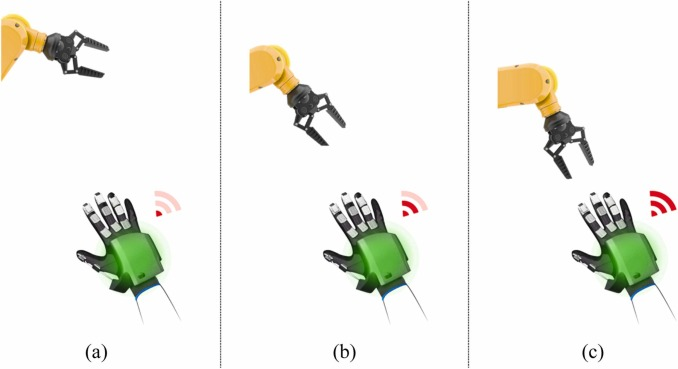
\includegraphics[width=0.7\linewidth]{figs/haptic-cues.jpg}
        \caption{Cues indicating the gripper’s destination using vibration on different human fingers.}
        \label{fig:sfig1}
    \end{subfigure}

    \vspace{0.5cm} % Adds space between the figures
    
    \begin{subfigure}{\textwidth}
        \centering
        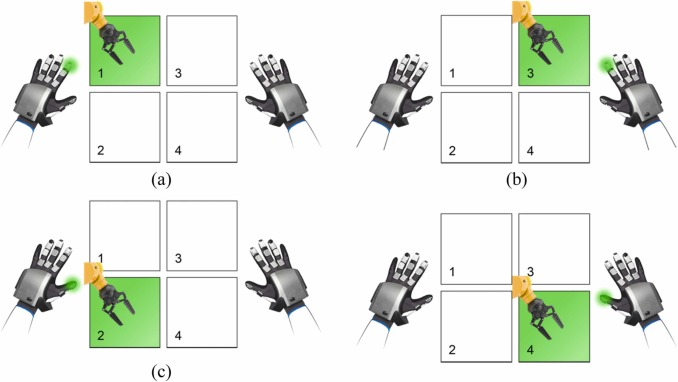
\includegraphics[width=0.7\linewidth]{figs/visual-cues.jpg}
        \caption{Cues indicating the proximity of the gripper via vibration frequency changes.}
        \label{fig:sfig2}
    \end{subfigure}
    
    \caption{Visual and haptic interfaces used in the experiment~\cite{CHU2023313}.}
    \label{fig:haptic-visual-cues}
\end{figure}


Findings show that combining visual, haptic, and acoustic cues significantly improve task performance. Visual interfaces, especially those indicating proximity, excelled in usability, while haptic feedback proved invaluable in scenarios where visual input was insufficient or overloaded. Acoustic signals also served as alerts for sudden changes in the robot's motion, helping reduce operator anxiety in unpredictable environments.

In a task where the operator and robot worked independently but in close proximity, the system enabled efficient coordination. The robot delivered materials while the operator performed assembly tasks, highlighting the potential for \ac{AR}-based interfaces to optimize \ac{HRC} in industrial settings.

\subsection{Augmented Reality-Assisted Multi-Robot Systems for Enhanced Control and Coordination}

Integrating \ac{AR} into multi-robot manufacturing systems offers significant improvements in interaction, operational safety, and efficiency, especially when applied to real-time and planned control modes. Ong et al.~\cite{ong2020} further explored \ac{AR}-assisted robot programming for welding applications, demonstrating that user-friendly interfaces can significantly reduce the complexity and duration of the programming process. These interfaces enable operators to define welding points and orientations using handheld pointers, thus enhancing task accuracy and efficiency by allowing validation within the actual robot workspace.

Malí et al.~\cite{7819154} developed an \ac{AR} application that permits users to adjust robot axis values, visualize specific robot points through 3D arrows, and navigate hidden points using leading lines. Evaluated in an industrial setting, this application showed improvements in usability and interaction capabilities.

Puljiz et al.~\cite{puljiz2019conceptsendtoendaugmentedreality,puljiz2} explored various \ac{AR}-based methods for robotic arm programming using devices like the Microsoft HoloLens, implementing techniques such as hand-guided task programming, augmented trajectory visualization, and the creation of spatial maps for virtual waypoint placement. These methods facilitate intuitive and accurate robotic arm programming, enabling seamless integration between virtual commands and real-world operations.

Modern manufacturing trends are characterized by a shift toward mass customization and increased flexibility, driven by the demand for individualized products. This necessitates more adaptable manufacturing systems where human operators collaborate with industrial robots to handle complex tasks~\cite{1-ar-dt,2-ar-dt,3-ar-dt}. However, existing robotic systems primarily execute pre-programmed tasks with limited intelligence.

To address this, two promising approaches have emerged: leveraging advanced \ac{AI} techniques for robot learning~\cite{6-ar-dt} and integrating a human-in-the-loop strategy for robot teleoperation. The latter, more aligned with Industry 5.0 principles, extends the capabilities of both humans and robots by incorporating human expertise into collaborative multi-robot processes~\cite{7-ar-dt}.

Unlike traditional \ac{HRC}, multi-robot manufacturing with a human in the loop allows operators to interact with robots from remote locations, not limited to physical workspaces. This paradigm facilitates safer and more flexible manufacturing, by bridging the gap between fully automated and manual operations~\cite{7-ar-dt}. However, significant challenges remain, including the need for more user-friendly teleoperation interfaces and systems that can be easily utilized by manufacturing operators without extensive robotics training~\cite{9-ar-dt}.

Research in multi-agent collaborative manufacturing has focused on enhancing safety, productivity, and cost reduction. Wearable \ac{AR}-assisted systems and \ac{DT} technologies enable accurate and intuitive robot teleoperation. By combining \ac{AR} with robot teleoperation, workers can access physical and virtual information simultaneously in a hybrid environment, interacting with virtual objects~\cite{26-ar-dt,27-ar-dt}. An example is an \ac{AR}-based teleoperation system utilizing RGB-D imaging, allowing operators to perceive the remote robot's environment and perform teleoperation~\cite{10-ar-dt}. Another system transforms robot workspaces into \ac{AR} environments for rapid and intuitive path planning and task programming~\cite{30-ar-dt}. These systems improve task performance by providing additional visual cues to enhance the operator's situational awareness.

Recent advancements in smart manufacturing have led to the development of \ac{DT} models for robot control. For example, \cite{37-ar-dt} used the Unity engine to create a \ac{DT} of a robot arm that could learn manufacturing tasks virtually and replicate them in the physical world. The integration of \ac{DT} and \ac{VR} interfaces has also been proposed to design immersive human-in-the-loop robotic systems, where the \ac{DT} acts as an intermediary layer for task execution and quality monitoring~\cite{41-ar-dt,42-ar-dt}.

Li et al.~\cite{LI2022102321} demonstrated how \ac{AR}-assisted \ac{DT} enable operators to manage and coordinate multiple robots more effectively.
Figure~\ref{fig:physical-digital} depicts an immersive dual view where users can interact with the physical setup of two collaborating robots while simultaneously observing their virtual counterparts through Microsoft HoloLens \ac{AR} glasses. This setup allows for real-time monitoring and simulation of manufacturing processes, improving robot operation control.

\begin{figure}[!htpb]
    \centering
    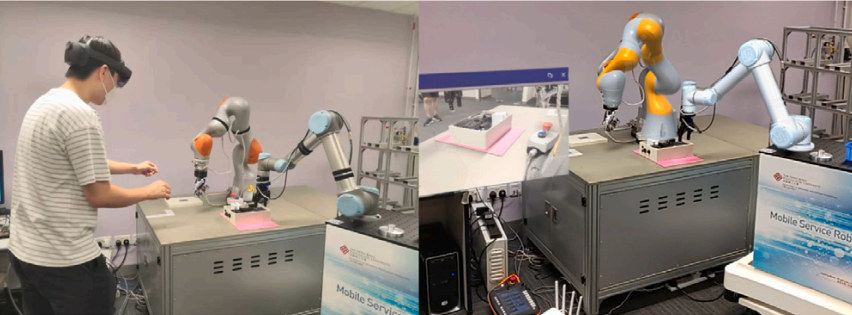
\includegraphics[width=0.85\linewidth]{figs/physical-digital.png}
    \caption{\ac{AR}-assisted \ac{DT}-enabled multi-robot collaborative manufacturing system~\cite{LI2022102321}.}
    \label{fig:physical-digital}
\end{figure}

Their proposed comprehensive framework for an \ac{AR}-assisted, \ac{DT}-enabled robot collaborative manufacturing system features human-in-the-loop control.  It includes the design of an \ac{AR}-based teleoperation system for pose registration and motion planning, coupled with three \ac{DT}-enabled interaction approaches to achieve closed-loop interaction between virtual and physical robots. The \ac{DT} of the physical robot, modeled using the Unity engine, is displayed as a hologram in the remote workspace via \ac{AR} glasses, enabling teleoperation and remote monitoring. Pose registration involves aligning the virtual and physical robot models using the Vuforia Engine, while joint alignment translates \ac{DT} joint values into real-world coordinates.

% The system architecture introduces a multi-node communication mechanism to facilitate interactions among multiple robots and clients.
% \begin{figure}[!htpb]
%     \centering
%     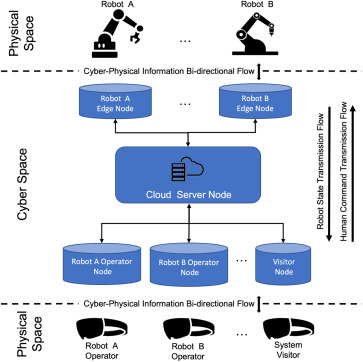
\includegraphics[width=0.5\linewidth]{figs/framework.jpg}
%     \caption{The architecture of a multi-robot, multi-client communication mechanism~\cite{LI2022102321}.}
%     \label{f:system-framework}
% \end{figure}

Therefore, a robot control approach aided by \ac{AR} technology offers several benefits:
\begin{itemize}
    \item Enhanced predictability of robot posture and motion trajectories.
    \item Trajectory visualization to prevent safety issues.
    \item An intuitive interface that overcomes spatial and physical limitations.
\end{itemize}

However, observing workspace and robot state information during task execution presents challenges, such as networking latency and positioning accuracy. Proposed solutions include time-sensitive networks and advanced communication technologies such as 5G~\cite{LI2022102321}.

The proposed system also utilizes \ac{IP} cameras for workspace monitoring, projecting video feeds onto \ac{AR} glasses for enhanced remote monitoring, as shown in Figure~\ref{f:workspace-visualization}.

\begin{figure}[!htpb]
    \centering
    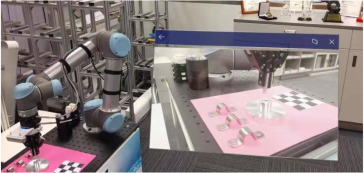
\includegraphics[width=0.7\linewidth]{figs/workspace-visualization.jpg}
    \caption{Demonstration of the workspace observation approach~\cite{LI2022102321}.}
    \label{f:workspace-visualization}
\end{figure}
\FloatBarrier


% Despite these advancements, challenges such as \ac{DT} model accuracy and network latency still affect the overall system performance. Addressing these limitations is essential for realizing the full potential of \ac{AR}-assisted \ac{DT} systems in industrial applications~\cite{LI2022102321}.


\section{Future Trends in Human-Robot Collaboration}

All in all, future directions in \ac{HRC} are evolving due to advancements in cobot technologies, sensing methodologies, and algorithmic developments \cite{robotics8040100}. The key trends identified include:

\begin{itemize}
    \item \textbf{Enhanced Scene Understanding:} Next-generation \ac{HRC} systems will prioritize deeper contextual awareness of the workspace and tasks at hand. This involves not only detecting the physical environment but also interpreting operator intentions, recognizing task progression, and continuously monitoring environmental dynamics. Such enhanced scene understanding will enable robots to anticipate human actions, predict potential safety risks, and adjust their behavior accordingly, thus fostering a higher level of operational safety and efficiency.

    \item \textbf{Advanced Sensing and Data Fusion:} To facilitate this enhanced scene understanding, advanced sensing methodologies and sophisticated data fusion techniques will be critical. By integrating multi-modal sensor data—such as visual, tactile, and auditory inputs—robots will be able to construct more comprehensive models of their surroundings and human collaborators. Real-time fusion of such data will allow systems to process information more effectively, ensuring safer interactions by predicting hazardous movements and improving overall system transparency. This, in turn, will enhance user trust and accelerate the adoption of \ac{HRC} solutions across industries.

    \item \textbf{Improved Task Planning and Adaptive Learning:} Future \ac{HRC} systems will be distinguished by advanced task planning capabilities, driven by more sophisticated task modeling and real-time adaptation mechanisms. As robots become more capable of autonomously learning from both structured and unstructured environments, their ability to handle a wider array of tasks will expand, reducing human involvement in routine planning stages. The deployment of these capabilities in manufacturing and service sectors will enable robots to shift between tasks seamlessly, dynamically adjusting their behavior to respond to real-time changes in production or workflow.

    \item \textbf{User-Friendly Interfaces and Interaction Methods:} As the complexity of \ac{HRC} systems increases, the need for intuitive and accessible human-robot interfaces will become paramount. Developing user interfaces that enable seamless human control without requiring advanced technical expertise is a key area of research. Implementing \ac{AR} and \ac{VR} technologies is expected to play a pivotal role in this domain, offering operators immersive and intuitive control mechanisms. These interfaces will reduce cognitive load and enable operators to interact with robots more effectively, thus improving operational efficiency and overall system usability.

    \item Among other relevant topics, which will not be further described due to not being the focus of this dissertation, incorporating \ac{ML} and adaptive learning algorithms into \ac{HRC} systems also represent a transformative leap forward.
    %  Techniques such as learning-by-demonstration, and \ac{RL} will enable robots to more accurately mimic human dexterity and decision-making processes, allowing them to learn from human input and adapt to non-repetitive, complex tasks. These adaptive systems will continuously improve based on interaction data, leading to more intuitive and efficient \ac{HRC} in dynamic industrial environments.
\end{itemize}


Historically, the focus has been on increasing the relevance of \ac{HRI} by addressing higher safety requirements and enabling 
robots to perform more complex tasks. Recently, the scope has expanded to include more sophisticated methods aimed at enhancing system performance, 
applying these methods across different application fields and tackling more intricate tasks. This expansion is driven by the emergence of new 
cobots, advancements in sensing technologies, matured algorithms, and accumulated experience in designing collaborative workcells \cite{robotics8040100}.

\section{Summary}

Even though significant advancements in \ac{AR}-\ac{DT} implementations over the past decade, the state-of-the-art literature predominantly focuses on developing applications for on-site personnel. Remote collaboration, particularly in \ac{HRC} scenarios, has received comparatively less attention, highlighting the need for systems that effectively facilitate both on-site and remote collaboration. Therefore, the proposed project aims to facilitate and integrate better remote collaboration by proposing a generalized conceptual system applicable across various application scenarios.

Despite having developed on-site features, such as \ac{DT} pose registration alongside audio and visual cues, focus will be mainly on the remote collaboration part implementation and the billateral communication between users. Unity 3D engine will be further explored for robot model development, \ac{ROS} will be used for robot control, and Vuforia for pose registration. It will also incorporate visual and audio cues to enhance user safety and awareness, as well as \ac{MR} elements implemented with Unity 3D. A camera will enable workspace monitoring. 

In conclusion, the proposed system will enable remote users to manipulate the robot using \ac{HHD}, with the robot's real-time position displayed in the Unity \ac{DT}. By addressing these challenges, the project aims to enhance remote collaboration in \ac{HRC} scenarios, contributing to the broader field of \ac{MR}-\ac{DT} applications.

% *TODO: check if below references are useful
% %add this part somewhere
% from article: 9911168
% "AI, AR, DT and HRC approaches are employed in smart manufacturing to transform data processing into digital processing and controlling. 
% Therefore, designing smart systems will lead to high-quality real-time data exchange, zero wasted efforts and better data management [43]. 
% Focusing on HRC applications, HRC is the future alternative to conventional robotic and automation systems."

% %also add this part somewhere:
% from article: chang-ar-hrc
% " Augmented reality will only continue to mature into
% a more accessible technology, and its role in human–robot collaboration can become much
% more impactful and relevant to many different domains"


% from chat - use this and remove the below future work and summary? - check this
% \section{Future Trends in Human-Robot Collaboration}

% As detailed in the 2019 article \textit{Human–Robot Collaboration in Manufacturing Applications: A Review}~\cite{robotics8040100}, the future of \ac{HRC} is shaped by ongoing advancements in collaborative robot technologies, sensing techniques, and algorithmic developments. These trends are instrumental in refining how robots and humans interact and collaborate. Key areas of development include:

% \begin{itemize}
%     \item \textbf{Enhanced Scene Understanding}: Future \ac{HRC} systems will prioritize comprehensive contextual awareness, encompassing not only environmental sensing but also interpreting human intentions, task progression, and monitoring dynamic changes. This will enable robots to predict human actions, detect potential risks, and adjust behaviors in real time, significantly improving operational safety and efficiency.

%     \item \textbf{Advanced Sensing and Data Fusion}: Achieving enhanced scene understanding necessitates sophisticated sensing methodologies and multi-modal data fusion. By integrating data from visual, tactile, and auditory sensors, robots can construct more nuanced models of their surroundings and human collaborators. Real-time data fusion will enable preemptive responses to hazards, enhancing safety and transparency, which are critical for increasing user trust in \ac{HRC} systems.

%     \item \textbf{Integration of Learning Techniques}: Incorporating \ac{ML} and adaptive learning algorithms is pivotal for advancing \ac{HRC}. Techniques such as reinforcement learning and learning-by-demonstration will empower robots to mimic human dexterity, adapt to non-repetitive tasks, and continuously improve from interaction data, leading to more intuitive and efficient collaboration.

%     \item \textbf{Improved Task Planning and Adaptive Learning}: The future of \ac{HRC} will be characterized by sophisticated task planning, supported by real-time adaptation mechanisms and complex task modeling. As robots become more adept at learning from structured and unstructured environments, their ability to seamlessly transition between tasks will reduce the need for human intervention in routine planning.

%     \item \textbf{User-Friendly Interfaces and Interaction Methods}: Given the rising complexity of \ac{HRC}, developing intuitive interfaces for non-expert users is essential. The implementation of \ac{AR} and \ac{VR} technologies will facilitate immersive, intuitive interactions, reducing cognitive load and improving system usability.
% \end{itemize}

% Overall, these emerging trends indicate a shift towards more intelligent, context-aware, and adaptive \ac{HRC} systems that prioritize both operational efficiency and user experience. Historically, the focus has been on enhancing safety standards and enabling robots to perform more complex tasks. This trajectory is now expanding, driven by advancements in cobots, sensing technologies, and algorithmic improvements, alongside accumulated experience in collaborative workcell design~\cite{robotics8040100}.

% \section{Summary}

% Despite the significant progress in \ac{MR}-\ac{DT} technologies, the state-of-the-art literature largely centers on on-site applications. The potential for enhancing remote collaboration, particularly within \ac{HRC}, remains underexplored. This gap highlights the need for systems that effectively integrate on-site and remote collaboration capabilities.

% The proposed project aims to address this gap by developing a generalized conceptual framework for remote collaboration in various scenarios. While on-site features such as digital twin pose registration and multimodal cues have been implemented, the primary focus will be on advancing remote collaboration and bidirectional communication between users.

% The project will leverage the Unity 3D engine for robot model development, \ac{ROS} for robot control, and Vuforia for pose registration. Visual and audio cues will be incorporated to enhance safety and situational awareness, with \ac{MR} elements integrated using Unity 3D. Additionally, a camera will provide workspace monitoring.

% Ultimately, the proposed system will empower remote users to manipulate the robot through \ac{HHD}, with real-time feedback displayed on the digital twin in Unity. By addressing these challenges, the project aims to advance remote collaboration in \ac{HRC}, contributing to the broader field of \ac{MR}-\ac{DT} applications.





\chapter{Methodology}%
\label{chapter:methodology}

As defined earlier in section~\ref{section:Goals}, the primary goal of this dissertation is to leverage the Human-Robot Collaboration \ac{HRC} paradigm by integrating \ac{MR} technologies alongside robot capabilities to enhance remote collaboration. In order to achieve this, a conceptual model is further implemented.

\section{Conceptual Model}
In order to start addressing the mentioned challenges, a first effort has been made. A robotic arm from Universal Robots, UR10e, shown in the figure \ref{f:ur10e_iris}, available at IRIS LAB, was used as a dynamic agent to assist in shared activities.
%  add a footnote to the robot model in universal robots website

\begin{figure}[h]
    \centering
    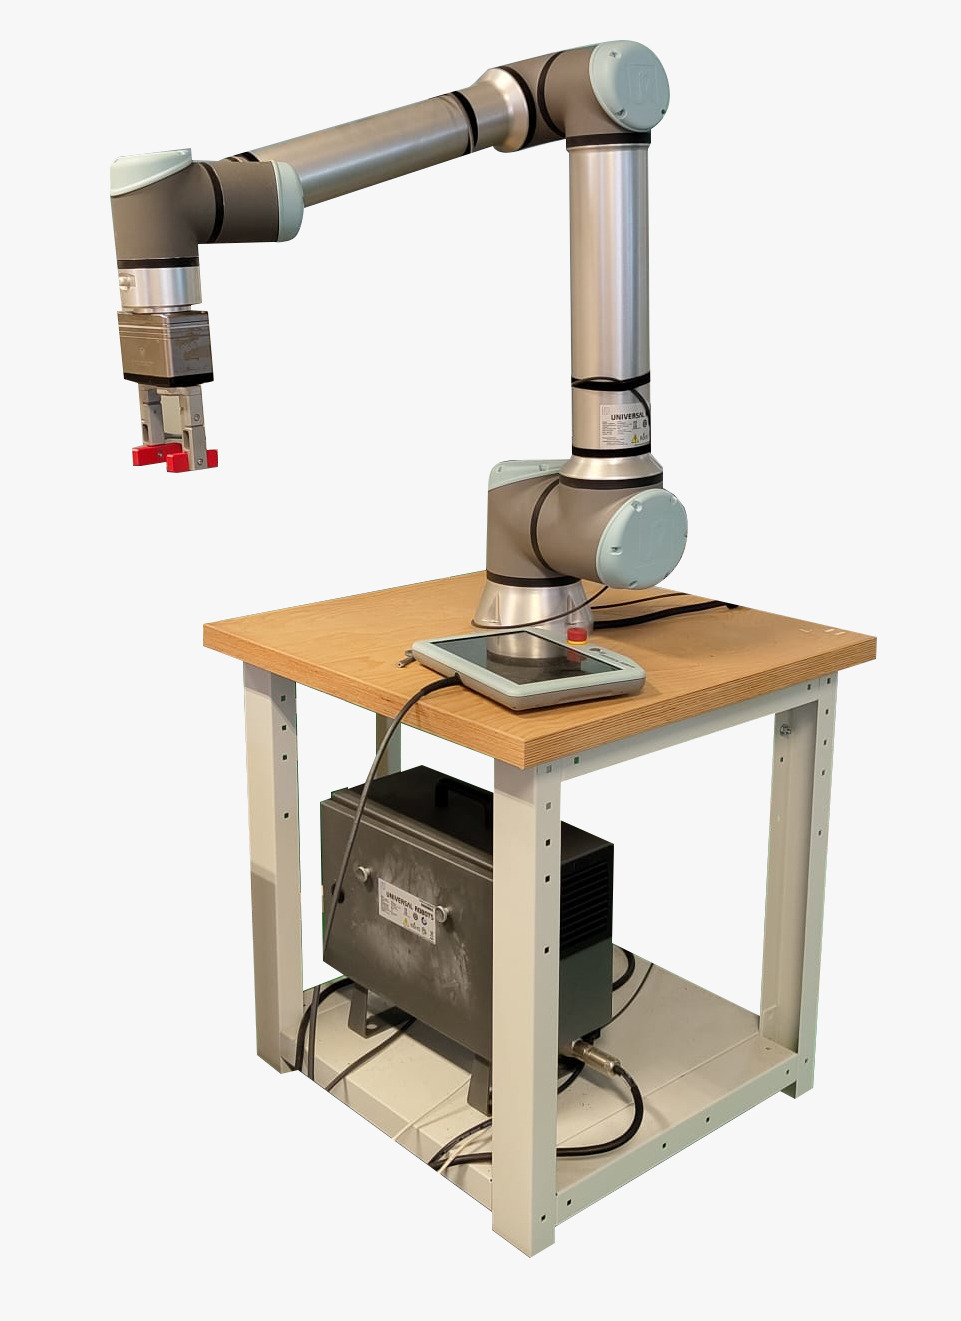
\includegraphics[width=0.4\linewidth]{figs/ur10e.jpeg}
    \caption{Robot UR10e used for the development of the dissertation work, available at IRIS-LAB, University of Aveiro}
    \label{f:ur10e_iris}
\end{figure}

Afterwards, the framework required to integrate the \ac{MR} technologies with the robotic arm was thoroughly discussed with the supervisors, leading to the following components:
\begin{itemize}
    \item \textbf{On-Site Interaction:}
    \begin{itemize}
        \item Implement an UR10e digital model into the Unity 3D simulation environment
        \item Utilize marker detection, utilizing Vuforia, to align the digital model with the physical robot
        \item Perform pose registration to ensure accurate spatial alignment between the virtual and physical models
        \item Develop a user-friendly interface for robot manipulation using \ac{HHDs}
        \item Implement visual and audio cues for user awareness and accident prevention 
    \end{itemize}
    \item \textbf{Remote Visualization and Interaction:}
    \begin{itemize}
        \item Enable bilateral communication between the robot and the Unity digital twin
        \item Provide remote participants with a foundational 2D interface, such as a laptop screen, to visualize the collaboration scenario and 
        task context.
        \item Implement real-time updates of the robot's position and workspace visualization
        \item Develop the capability for remote operation of the robot via the \ac{MR} application, enhancing the remote participant's ability to 
        interact and manipulate the collaborative environment.
    \end{itemize}
    \item \textbf{Automation and Immersion:}
    \begin{itemize}
        \item Integrate a camera into the robot and develop a camera feed transmission to provide real-time updates of the robot's position and workspace visualization
        \item Share this information with remote participants, assisting on-site participants by delegating visual sharing to the robot.
    \end{itemize}
\end{itemize}



\section{Digital Model Implementation of the Robot}
\label{section:digital-model}

\subsection{Unity}



Unity is a dynamic and versatile game engine developed by Unity Technologies \footnote{Unity Technologies \url{https://unity.com/} Accessed: 2024-09-30}, widely recognized for revolutionizing game development over the past few years. Beyond gaming, it has become a prominent tool for creating \ac{AR}, \ac {VR}, and \ac{MR} applications. Its user-friendly interface empowers developers to rapidly craft immersive experiences while simplifying complex development processes.

By offering an \ac{IDE} that combines \ac{GUI} manipulation of scene objects with a code editor, similar to Visual Studio, it allows developers to build virtual scenes by either creating or integrating 2D and 3D assets as well as apply attributes such as lighting, audio, physics properties, animations, and interactive gameplay logic. Afterwards, these composed scenes come to life, rendering them in real-time at frame rates that create smooth motion and immersive experiences.

One of Unity's significant advantages is its extensive platform compatibility. It supports development for various operating systems, including Windows, and Linux, as well as mobile platforms like iOS and Android. Additionally, a wide range of devices spanning \ac{AR},\ac{VR},\ac{MR} technologies are supported.

Unity's choice for developing the \ac{MR} application was advised by both supervisors regarding its versatility as well as its robust capabilities and extensive feature set.

\subsection{Digital Robot Model - URDF Importer Package}
% % % foi necessário encontrar um modelo do robot a ser utilizado - UR10e que se encontra no IRIS lab
% To successfully develop the XR application for controlling the UR10e robot, it was essential to identify a model that closely mirrors 
% the actual robot. The Unity Robotics Hub \footnote{Unity Technologies \url{https://github.com/Unity-Technologies/Unity-Robotics-Hub} 
% Accessed: 2024-02-02} facilitates the integration of robotics into Unity projects via the URDF-Importer package 
% \footnote{Unity Technologies \url{https://github.com/Unity-Technologies/URDF-Importer} Accessed: 2024-02-02}. 
% However, challenges arose when attempting to import the UR10e \textit{.urdf} model into the Unity environment. To overcome this, 
% a UR10 model, sourced from a GitHub repository \footnote{PositronicsLab \url{https://github.com/PositronicsLab/reveal_packages/tree/master/industrial_arm/scenario/models/urdf/ur10} Accessed: 2024-02-05} 
% was used, due to its resemblance to the UR10e robot. This was discussed with the educators overseeing the dissertation development, 
% and it was agreed that this approach would not pose any issues.

% In the figure \ref{f:ur10_marker_unity} it is possible to see the digital UR10 model positioned related to the aruco marker 
% (\ref{f:aruco_marker}), in a simulated Unity environment.
% \begin{figure}[h]
% \centering
% 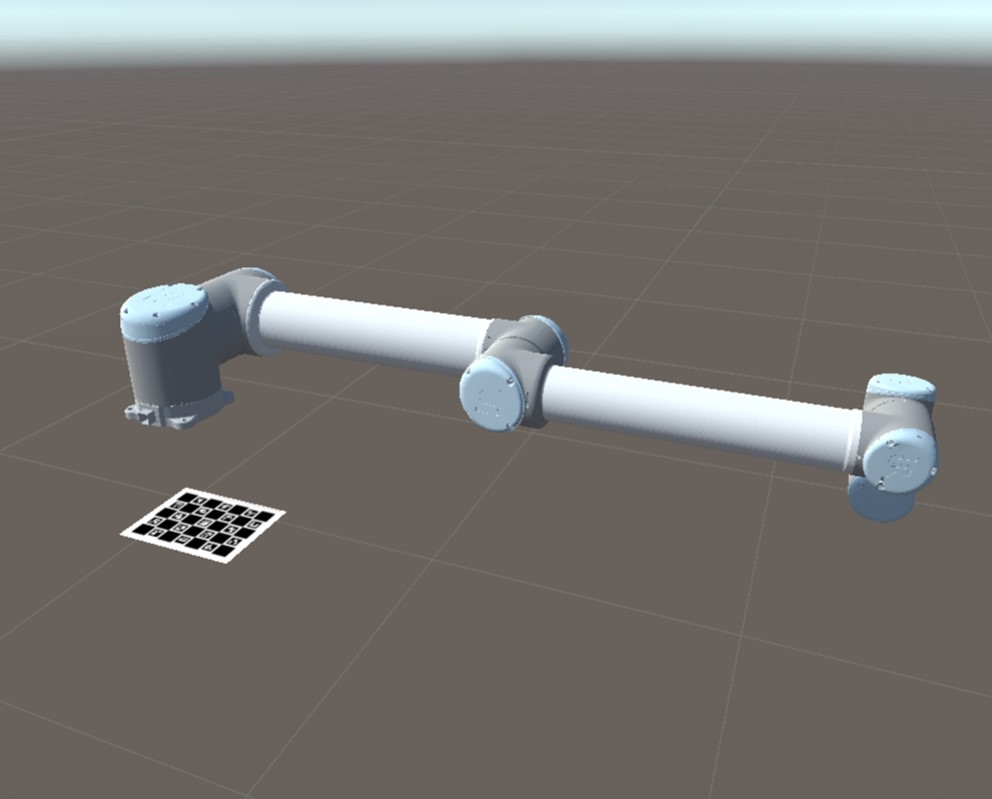
\includegraphics[width=0.6\textwidth]{figs/robot_marker_unity.jpg}
% \caption{Digital UR10 model related to the aruco marker, on Unity environment}
% \label{f:ur10_marker_unity}
% \end{figure}
 - commented this part because text is below - choose whether to use this or the text below

    % foi necessário encontrar um modelo do robot a ser utilizado - UR10e que se encontra no IRIS lab
    To successfully develop the \ac{MR} application for controlling the UR10e robot, it was essential to identify a model that closely mirrors 
    the actual robot. The Unity Robotics Hub \footnote{Unity Robotics Hub \url{https://github.com/Unity-Technologies/Unity-Robotics-Hub} 
    Accessed: 2024-02-02} facilitates the integration of robotics into Unity projects via the URDF-Importer package 
    \footnote{Unity URDF Importer \url{https://github.com/Unity-Technologies/URDF-Importer} Accessed: 2024-02-02}. 
    
    However, instead of importing the UR10e \textit{.urdf} model into the Unity environment, a UR10 model, sourced from a GitHub repository \footnote{PositronicsLab \url{https://github.com/PositronicsLab/reveal_packages/tree/master/industrial_arm/scenario/models/urdf/ur10} Accessed: 2024-02-05} 
    was used, due to its resemblance to the UR10e robot. 
    % This was discussed with the educators overseeing the dissertation development, and it was agreed that this approach would not pose any issues.


% \ac{MR} alongside a static robotic arm (UR10e) to support remote collaboration scenarios. This involves transforming human-robotic collaboration by integrating \ac{MR} technologies and robotic capabilities to enhance both on-site and remote collaboration experiences.

% Unity 3D engine will allow robot model development, enabling detailed and interactive digital twins with bilateral communication capabilities. By utilizing Vuforia for precise pose registration, the system ensures accurate spatial alignment between the virtual and physical robots.

% To enhance user awareness and prevent accidents, the system will implement visual and audio cues within the \ac{AR} environment, including safety-zone interactions and audio alerts. These features provide intuitive feedback to users, improving situational awareness during human--robot collaboration. The robot manipulation interface will be designed to be user-friendly, allowing non-expert users to operate the robot remotely using a handheld device (\ac{HHD}). This accessibility ensures that a wider range of users can effectively interact with the robotic system without extensive training.

% Real-time updates of the robot's position and workspace visualization will be provided through camera feed transmission, offering remote users a comprehensive view of the operational environment. This feature addresses the limitations identified in existing literature, where remote users often lack sufficient context and visibility of the workspace.

% % Furthermore, the proposed system will address challenges identified in the state-of-the-art review, such as networking latency and positioning accuracy. By implementing optimized communication protocols and advanced tracking algorithms, the system aims to ensure efficient and safe human--robot collaboration. These improvements will not only enhance the performance of the system but also contribute valuable insights to the field, bridging the gap between on-site and remote interaction capabilities in industrial applications.

% Overall, this project seeks to expand upon current research by providing a holistic solution that integrates advanced technologies to facilitate seamless collaboration between humans and robots, regardless of physical location. By focusing on both on-site and remote users, the system aims to enhance flexibility, safety, and efficiency in various industrial scenarios.

\section{Pose registration}

After having successfully imported the \ac{URDF} model of the real robot into the Unity environment, the next step was to ensure that the digital model was accurately aligned with the physical robot. 

\subsection{Vuforia}
\label{section:marker-detection}
% 
% Vuforia is a software platform that enables the creation of \ac{ar} experiences. 
% % Integrated with Unity, a leading platform for developing games and interactive applications, Vuforia simplifies the incorporation 
% of AR into mobile and digital apps. 
% It uses computer vision technologies to recognize and track images and objects in the real world, allowing developers to overlay digital 
% content precisely.

% The marker illustrated in Figure \ref{f:aruco_marker} was selected following initial attempts that yielded inconsistent results when using 
% the laptop's camera, shown in the figure \ref{fig:camera-c922}, to scan the environment. This particular marker demonstrated greater stability, 
% enabling the precise positioning of the digital UR10 model in alignment with the physical surroundings. Consequently, this facilitated the accurate 
% overlay of the digital UR10 model onto the actual UR10e robot, enhancing the integration of virtual and real-world elements.

% \begin{figure}[h]
%     \centering
%       \begin{subfigure}[b]{0.45\textwidth}
%       \centering
%       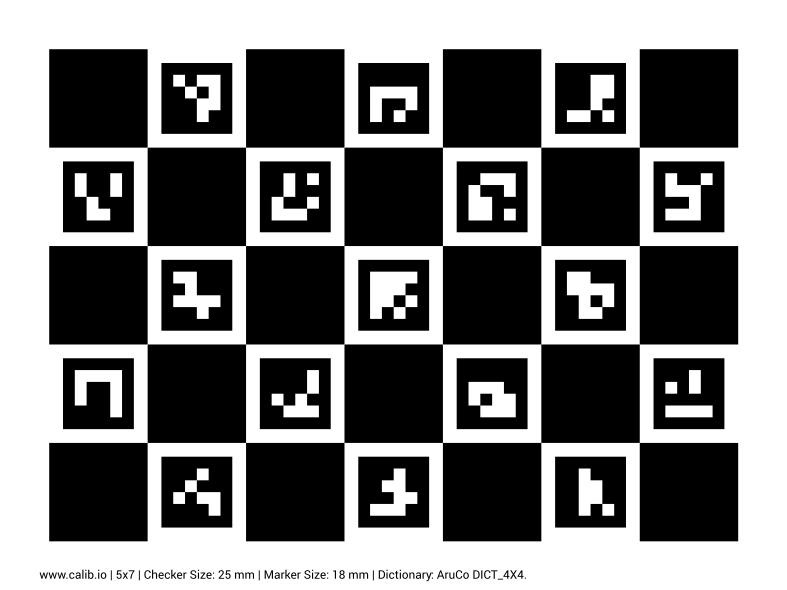
\includegraphics[width=0.7\textwidth]{figs/calib_io_charuco_200x150_5x7_25_18_DICT_4X4.png}
%       \caption{ArUco marker used to allow the segmentation for aligning the digital twin accordingly to the real environment}
%       \label{f:aruco_marker}
%       \end{subfigure}
%         \hfill % This command adds space between the subfigures
%       \begin{subfigure}[b]{0.45\textwidth}
%           \centering
%           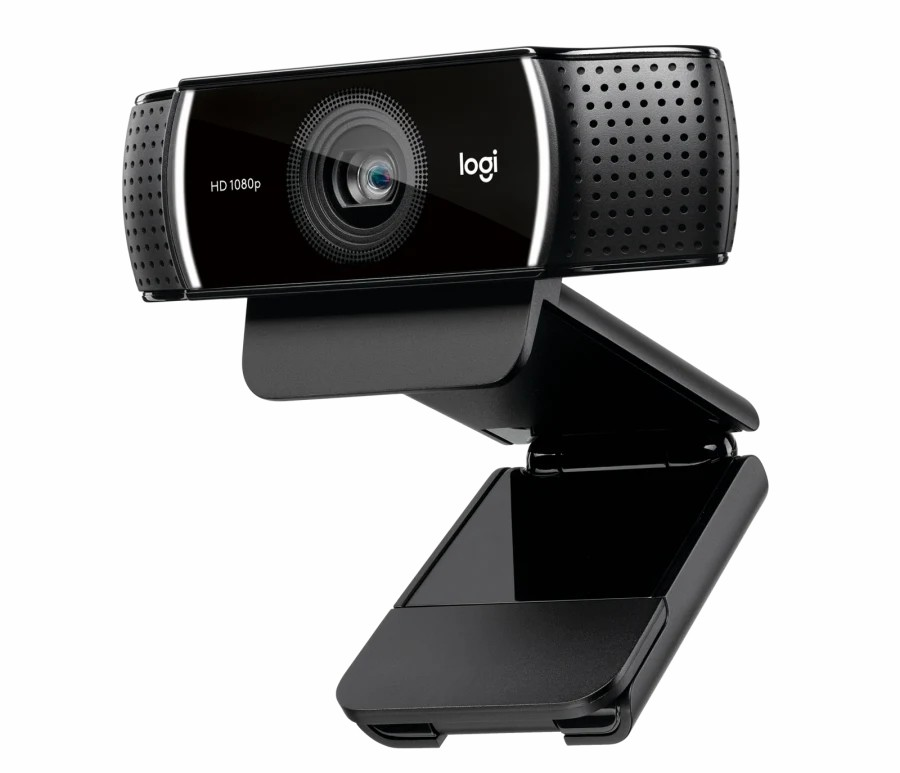
\includegraphics[width=0.7\linewidth]{figs/camera-c922.jpg}
%           \caption{Logitech c922 camera, used for testing on-site application developments}
%           \label{fig:camera-c922}
%       \end{subfigure}
%       \caption{ArUco marker used with the Logitech c922 camera for segmentation and manipulation of virtual environment}
%   \label{marker-camera}
%   \end{figure}
   commented this part because text is below - choose whether to use this or the text below

This alignment was achieved by utilizing Vuforia, a software platform that enables the creation of \ac{AR} experiences. Integrated with Unity, Vuforia simplifies the incorporation of \ac{AR} into mobile and digital apps. It uses computer vision technologies to recognize and track images and objects in the real world, allowing developers to overlay digital content precisely.

\subsection{Marker Detection}

The marker illustrated in Figure \ref{f:aruco_marker}, demonstrated greater stability, enabling the precise positioning of the digital UR10 model in alignment with the physical surroundings. Its choice followed initial attempts that yielded inconsistent results while using some other ArUco generated examples \footnote{ArUco Markers Generator \url{https://chev.me/arucogen/} Accessed: 2024-09-30}. 

To scan the physical environment around the robot, the camera shown in the figure \ref{fig:camera-c922} was used throughout the features' development process. 

\begin{figure}[h]
    \centering
    \begin{subfigure}[b]{0.45\textwidth}
    \centering
    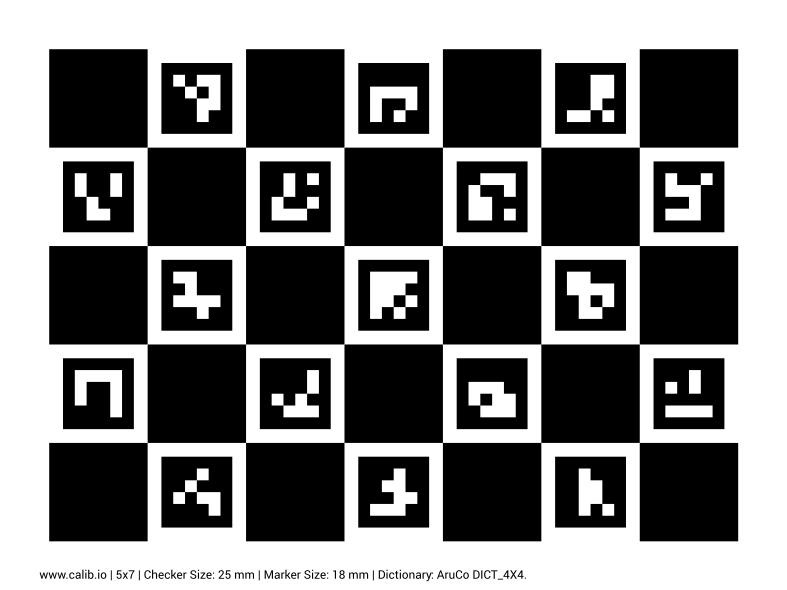
\includegraphics[width=0.7\textwidth]{figs/calib_io_charuco_200x150_5x7_25_18_DICT_4X4.png}
    \caption{ArUco marker used to allow the segmentation for aligning the digital twin accordingly to the real environment}
    \label{f:aruco_marker}
    \end{subfigure}
        \hfill % This command adds space between the subfigures
    \begin{subfigure}[b]{0.45\textwidth}
        \centering
        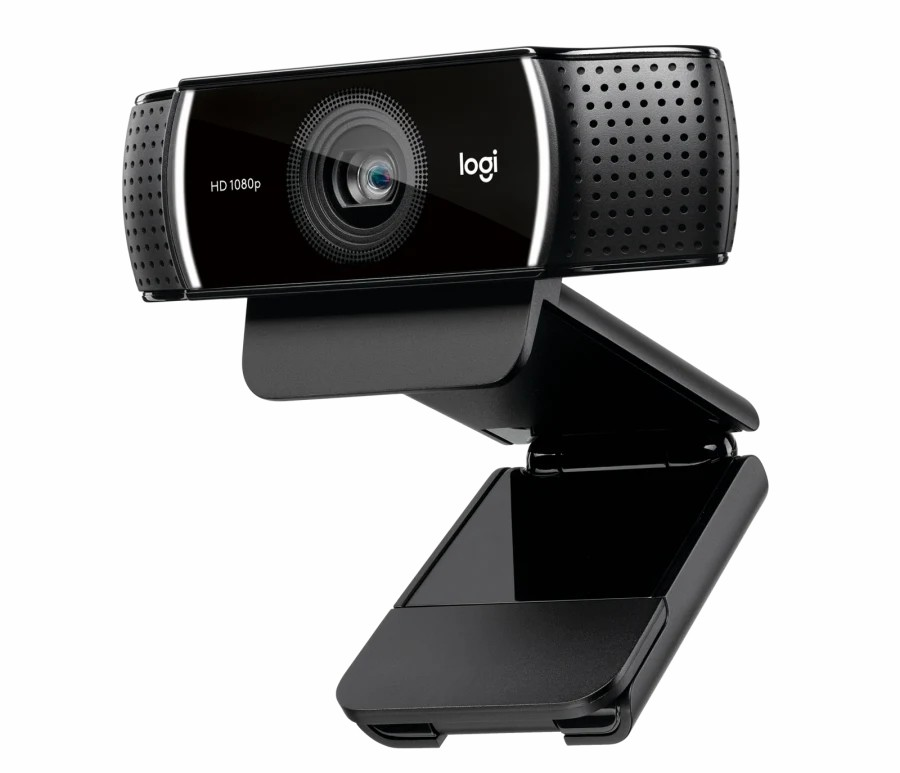
\includegraphics[width=0.7\linewidth]{figs/camera-c922.jpg}
        \caption{Logitech c922 camera, used for on-site integration}
        \label{fig:camera-c922}
    \end{subfigure}
    \caption{ArUco marker used with the Logitech c922 camera for segmentation and manipulation of virtual environment}
\label{marker-camera}
\end{figure}

Consequently, both the ArUco marker and the Logitech c922 camera allowed to overlay the digital UR10 model on top of the physical robot.
% enhancing the integration of virtual and real-world elements - use???????

In the figure \ref{f:ur10_marker_unity} it is possible to see the digital UR10 model positioned related to the aruco marker. 
    (\ref{f:aruco_marker}), in a simulated Unity environment.
    \begin{figure}[h]
    \centering
    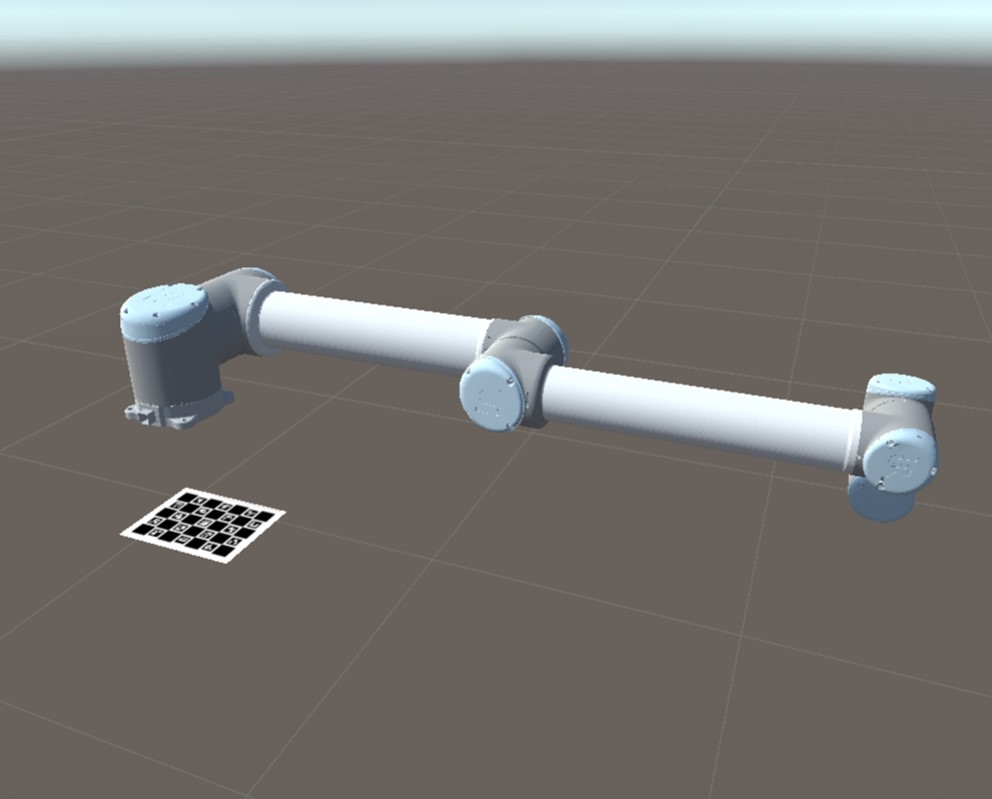
\includegraphics[width=0.6\textwidth]{figs/robot_marker_unity.jpg}
    \caption{Digital UR10 model related to the aruco marker, on Unity environment}
    \label{f:ur10_marker_unity}
    \end{figure}

\section{Billateral Communication}

\subsection{UR10e ROS Documentation}
Unity was chosen for its interactive capabilities, but this choice introduced additional complexity due to the need to operate across different operating systems—Windows for Unity and Ubuntu 20.04 for ROS Noetic, the version supporting the required ROS packages.

A key advantage was the existence of pre-existing resources from the IRIS Lab, where the robot is housed. Specifically, there were two GitHub repositories—\href{https://github.com/iris-ua/iris_sami}{iris\_sami} and \href{https://github.com/iris-ua/iris_ur10e}{iris\_ur10e}. These provided a well-established ROS environment, enabling control of the UR10e robot through RViz, trajectory planning, and real-time execution. \texttt{iris\_ur10e} package is integral to operating the physical robot in the lab, while \texttt{iris\_sami} allows for the robotic arm's manipulation.

Given this existing ROS setup on Ubuntu 20.04, ROS-TCP-Connector and ROS-TCP-Endpoint packages from the Unity Robotics Hub (\href{https://github.com/Unity-Technologies/ROS-TCP-Connector}{Unity-Technologies/ROS-TCP-Connector}) were used to establish the Wi-fi Connection. 

The proposed framework for both laptops connection is shown in figure. (add a figure of the framework proposed).


% Selecting this package over other ROS-Unity bridges was recommended by João Alves, one of the instructors who provided valuable insights during the development of this project.


\subsection{Message Generation}

By having already established the communication between Unity and ROS, specific types of messages from ROS environment had to be exchanged between the network, therefore enabling the robot to be controlled remotely.

After understanding that the ROS topic responsible for publishing the current state of the robot's joints was \texttt{/joint\_states}, these data needed to be sent to Unity. By adapting the already existing Unity Robotics Hub packages, these messages were not only successfully exchanged between the two environments, but also saved into a \texttt{.json} file for further manipulation.

\section{Robot Manipulation}
When it it came to control the digital version of the robot in the Unity environment, it was necessary to understand the Unity Robotics Hub package's way of doing so. A C\# script named \texttt{Controller.cs}, contained the necessary functions to control the robot's joints.


After further analysis, three control methods were implemented to control the robot's joints:
\begin{itemize}
    \item \textbf{UI Control:} This method allowed the user to control the \ac{DT} version of the robot by moving each joint individually through an Unity \ac{UI}. Its purpose consisted on being user-friendly and intuitive manner of controlling the robot, where a panel with a button for each joint was displayed, as shown in figure \ref{f:ui-control}. 
    
    \begin{figure}[h]
        \centering
        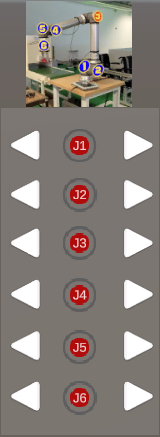
\includegraphics[width=0.6\textwidth]{figs/toggle-1.png}
        \caption{\ac{UI} panel to control the robot's joints individually}
        \label{f:ui-control}
    \end{figure}

    Besides the joints' buttons, a figure of the robot is also displayed in the top part of the panel, showing each joint's relative number, and thus allowing an easier identification of the joint to be controlled.
    
    Upon activating a joint by pressing the desired button, its color turns green instead of the default red button and the user is able to choose between rotating this joint in either the positive or negative direction, also represented by a change in the default color of the corresponding directional arrow. These features are represented in figure --- add figures joint being selected as well as the direction of UI control.
    
   
    \item \textbf{Unity-ROS Control:} This method enabled the robot to be controled during the runtime simulation in the Unity environment via the keyboard arrows of the laptop and then send the current position of the \ac{DT} into the ROS environment via Wi-fi and, consequently, update the robot's real position. 
    In order change the \ac{DT} robot state, the user had to press either the right or left arrow keyboard keys to select the following or previous joint, respectively, and the up or down arrow keys to rotate the selected joint in the positive or negative direction.
    After updating the \ac{DT} robot state, the user had to press the publish \ac{UI} button, that was added to the Interface, and the current joint states would be sent over Wi-fi to the ROS environment, which would then be constantly listening to the desired topic and upon receiving a new message, would then update the real robot with those values.
    



    \item \textbf{Remote Control:} This method allowed the robot to be controlled remotely by using the \ac{HHD}.

Firstly a \ac{UI} was desgined to allow the on-site member to control each robot joint individually by using an 



to understand that the \texttt{Controller.cs} script was responsible for controlling the robot's joints. This script was then adapted to allow for the robot's joints to be controlled using the \ac{HHD}.





\chapter{Mixed Reality for Human-Robot Collaboration}   
\label{chapter:on-site}
% \chapter{On-site Member's Application}% first title of section

\begin{introduction}
    % This chapter presents the development of a comprehensive framework for implementing a Mixed Reality environment in Human-Robot Collaboration. 
    % % By allowing both on-site and remote manipulation through a communication pipeline, this system enables real-time robot manipulation and monitoring. 
    % The framework leverages advanced technologies such as Mixed-Reality, Digital Twins, and ROS, ensuring precise synchronization between physical and digital models. It discusses the tools, control methods, and User Interface enhancements designed to optimize both on-site and remote user experiences, aiming towards an intuitive, immersive collaboration.
    The primary objective of this project is to enhance remote human-robot collaboration through a framework incorporating a UR10e robotic arm and a mixed reality interface. This framework leverages real-time, bidirectional communication, allowing the mixed-reality system to function as an active, synchronized digital twin rather than a static digital replica. With an intuitive user interface, the system aims to provide remote operators with robust visualization and precise control capabilities as well as enabling seamless monitoring and manipulation of the robotic arm within the collaborative environment
\end{introduction}


\section{System Framework and Architecture}

This section details the foundational architecture enabling seamless \ac{MR} integration within the \ac{HRC} environment, connecting on-site and remote interactions. Figure~\ref{fig:project_framework} illustrates the proposed framework of the system, through a robust communication pipeline designed to enable real-time, collaborative robot manipulation.

\begin{figure}[h]
    \centering
    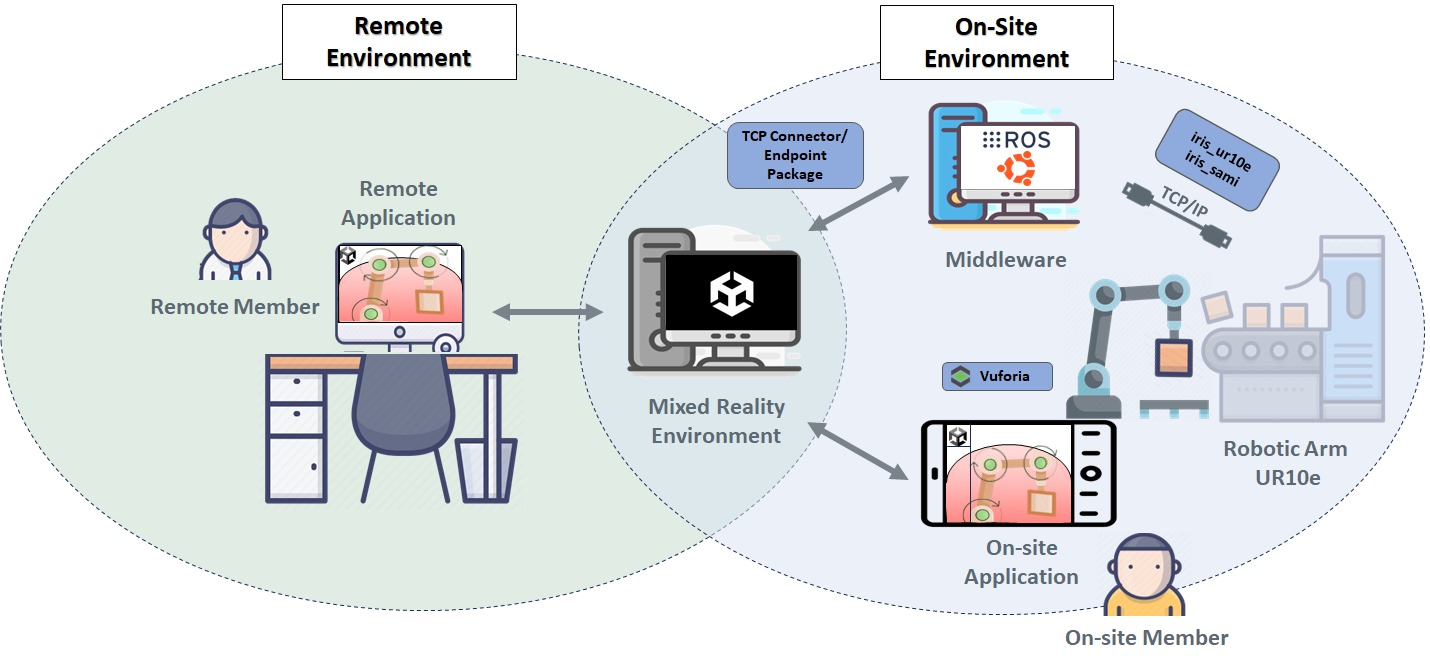
\includegraphics[width=\linewidth]{figs/framework-1.jpeg}
    \caption{Overview of the proposed \ac{MR}-based \ac{HRC} system framework integrating remote and on-site environments.}
    \label{fig:project_framework}
\end{figure}

First of all, regarding the \textbf{On-Site Environment}, the UR10e robotic arm operates as the central physical entity to be controlled. The on-site user controls this robotic arm through a custom \ac{MR} application, designed to create an immersive and interactive environment. It allows this user to stream the environment to the remote counterpart and intuitively manipulate the robot in real-time, as well as interact with the developed augmented features.  

After implementing the robot's digital model into the simulation environment, the next step was to align it with the physical robot. Pose registration between the physical robot and its digital counterpart is executed using Vuforia's capabilities. The system employs ArUco markers for precise pose estimation, ensuring that the digital representation of the UR10e is accurately aligned with its physical counterpart. The \ac{DT} of the robot, rendered in Unity, provides a visually synchronized, real-time mirror of the robot's movements and configurations, thus facilitating enhanced interaction.

The robot is connected via Ethernet to a laptop running Ubuntu 20.04 with \ac{ROS} Noetic, which serves as the middleware layer. This setup facilitates seamless data exchange between the Unity \ac{DT} and the physical robot. The \texttt{iris\_ur10e} and \texttt{iris\_sami} \ac{ROS} packages, available on IRIS Lab's GitHub~\footnote{https://github.com/iris-ua}, provide a pre-established \ac{ROS} environment that supports critical functionalities such robotic manipulation and visualization through RViz.

To tailor these packages to the specific needs of this project, several enhancements were made. These modifications included the integration of bidirectional data flow between \ac{ROS} and Unity, enabling the Unity-based \ac{DT} to mirror the real-time movements of the physical robot. In particular, new \ac{ROS} nodes were created to subscribe to joint state data from the physical robot and publish these updates to Unity, ensuring precise synchronization between the physical and virtual environments. Additionally, new publishing mechanisms were implemented to send commands from Unity back to \ac{ROS}, allowing for full control of the robot through the \ac{MR} interface. 

This communication between the \ac{ROS} middleware and Unity’s \ac{MR} environment is established using Unity’s \ac{ROS}-\ac{TCP}-Connector and \ac{ROS}-\ac{TCP}-Endpoint packages. These packages establish communication over a \ac{TCP}/\ac{IP} protocol, ensuring real-time synchronization between the virtual and physical environments. This architecture is fundamental for maintaining the \ac{DT}'s fidelity, reflecting real-world changes in the Unity model and vice versa, as referred in the section \ref{sec:dt}.

When talking about the \textbf{Remote Environment}, this user accesses the same Unity-\ac{MR} application, allowing it to visualize and manipulate the robot from a separate location. The \ac{UI} provides real-time visualization of the robot’s state and its workspace, enabling remote collaboration. The synchronization between the remote and on-site environments is facilitated through Unity’s \ac{MR} capabilities, which, in conjunction with the \ac{ROS}-based control, enables the remote user to execute commands and receive real-time feedback.

The Middleware layer, acting as the system’s backbone, ensures the continuous synchronization of data between the physical robot and its \ac{DT}. It manages the real-time feedback loop, maintaining bidirectional data flow between the virtual robot in Unity and the physical robot in the on-site environment. This configuration guarantees that any actions performed by either the on-site or remote user are consistently reflected in both the physical and digital realms, preserving operational coherence and maximizing collaborative efficiency.

This framework aims to provide an immersive and responsive \ac{MR} environment, bridging the gap between physical and digital spaces. The system enables real-time robot manipulation and monitoring from both on-site and remote locations, making it a versatile platform that could be used for collaborative tasks in advanced industrial applications. Seamless integration between \ac{MR} and \ac{DT} within \ac{HRC} technologies significantly enhances user interaction, safety, and productivity, while offering an intuitive interface for remote and on-site collaboration.


\section{Robot Manipulation Within Mixed Reality Environment}

Building on this comprehensive framework, the Unity-based \ac{MR} environment is designed to implement and control the \ac{DT} representation of the UR10e robotic arm. Initially, basic robot manipulation was achieved through the Unity Robotics Hub's \ac{URDF} Importer, enabling joint-specific adjustments via keyboard controls. However, to enhance user interaction and provide a more intuitive experience, new control methods were subsequently developed within the application, aimed at optimizing the user’s ability to monitor and interact with the robotic arm in real time. This section outlines these control methods in detail, describing their specific functions and contributions to the \ac{HRC} experience. 

In order to properly develop new ways of controlling the \ac{DT} version of the robot, it was necessary to understand the core C\# script which contained all the necessary functions to control the robot's joints within Unity, named \texttt{Controller.cs}. After further analysis, control methods were implemented to facilitate the manipulation of the digital robot model through a \ac{HHD} interface. This interface includes a menu displaying each joint, enabling users to adjust the robot’s position directly. Once the digital model is set to the desired position—either via the \ac{HHD} or keyboard controls—the user can publish this position to the \ac{ROS} middleware, which moves the physical robot accordingly. Additionally, another method was created for situations where the on-site counterpart manipulates the physical robot directly. In these cases, the \ac{DT} mirrors the real robot’s movements, maintaining synchronized operation between the physical and virtual environments. These methods are explained in detail below.


\subsection{UI Control Panel and Joint Manipulation}
\label{subsection:ui-control-method}
% \textbf{UI Control Method}:
This method is designed to provide users with an intuitive, user-friendly interface for manipulating the \ac{DT} of the UR10e robot. Figure \ref{f:ui-control} illustrates the \ac{UI} developed in Unity, highlighting its primary control panel on the left (1), which includes a detailed joint selection menu, directional arrows, and a reference image of the robot with joint labels (2 and 3). This panel is central to controlling the digital model of the robot, while other \ac{UI} features will be explained in subsequent sections.

\begin{figure}[h]
    \centering
    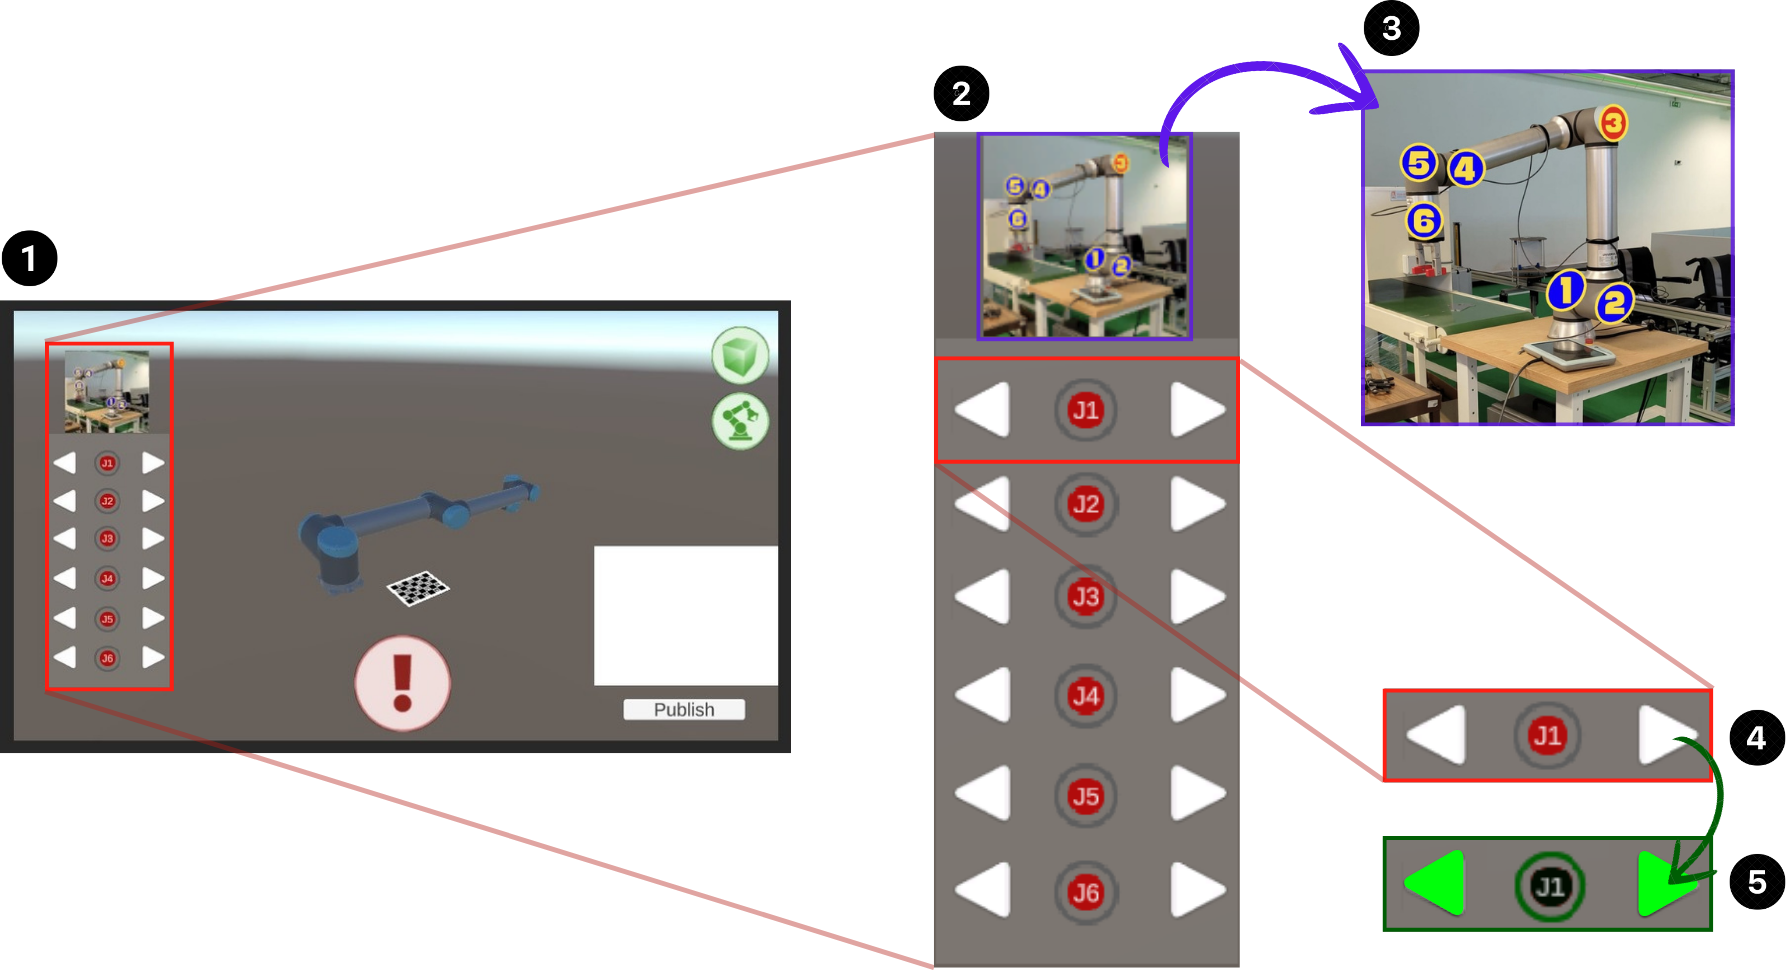
\includegraphics[width=\textwidth]{figs/interface-numerada-2.png}
    \caption{\ac{MR} \ac{UI} in Unity simulation environment (1). The control panel (2) enables the manipulation of the UR10e robot digital model. Users can manipulate each joint individually, with active joints displayed in green to indicate selection (5). The reference image of the robot (3), labeled with joint numbers (J1 to J6), aids in joint identification from base to end-effector. Directional arrows for each joint (2,4,5) facilitate movement control in positive or negative directions, offering intuitive joint-level manipulation within the simulation.}
    \label{f:ui-control}
\end{figure}


\textbf{Interface Structure and Joint Manipulation}:
\begin{itemize}
    \item \textbf{Joint Selection:} Each joint has a central button labeled with its identifier (e.g., J1, J2). To activate a joint, the user clicks the corresponding button, which changes color from red to green, signaling that the joint is selected for movement (4 and 5). This selection process helps avoid confusion and accidental manipulation of multiple joints.

    \item \textbf{Movement Control:} Once a joint is selected, the user can manipulate its position by clicking the directional arrows on either side of the central button. Pressing the right arrow rotates the joint in the positive direction, while the left arrow rotates it in the negative direction. This control mirrors the real-time responsiveness typically provided by keyboard arrows, ensuring an intuitive experience.

    \item \textbf{Continuous Movement:} The selected joint will continue moving in the chosen direction as long as both the central control button and the directional arrow remain selected. To stop the movement, the user can deselect either the joint by clicking on the central button or its rotational arrow, reverting these elements to its default color.

    \item \textbf{Single Joint Activation: }Only one joint can be active for rotation at any time. If multiple joints are selected (i.e., their buttons are green), the system prevents movement in any direction until only one joint is selected.

    % \item \textbf{Directional Exclusivity}: When a rotation direction is chosen (e.g., pressing the right arrow), the opposite direction is temporarily disabled, as shown in Figures 4 and 5. This feature prevents conflicting commands, reinforcing safe and logical control of the robot.
\end{itemize}

\newpage

\textbf{Additional Design Considerations: }
\begin{itemize}
    \item \textbf{Visual Reference for Joint Positioning:} The overlay image at the top of the joint control panel serves as a quick-reference guide for users to confirm joint positions relative to the physical robot. This visual aid is useful in remote collaboration or complex tasks where clear identification of each joint’s location is essential.

    % \item \textbf{UI Responsiveness and Feedback:} To ensure a smooth interaction, the interface provides visual feedback for each action (e.g., button color changes) and restricts movement based on user inputs, making the control process both transparent and manageable.
\end{itemize}

This structured approach to joint manipulation tries to promote safe, precise, and efficient interaction with the robot, supporting the usability goals of the \ac{MR} application. By minimizing the likelihood of accidental commands and providing continuous, clear visual feedback, the interface helps maintain control clarity and operational awareness throughout the interaction.
% The design is especially advantageous in collaborative environments, where multiple participants may need to observe and understand the robot’s operations in real time.


\subsection{Unity to Robot}
% \textbf{Unity-ROS Control:} 
Similarly to the previous described method, this one also enables the digital robot model to be controled from the \ac{MR} environment. However, when needed, it sends the newly defined digital robot position into the Middleware environment, updating the real UR10e robot status. In order to change the \ac{DT}, the user has can also do it by pressing the right/left arrow keyboard keys to select the following/previous joint as well as the up/down keys to rotate the selected joint in the positive/negative direction, respectively.
        
After moving the digital model to the desired position, by pressing the "Publish" button within the \ac{UI}, as shown in Figure \ref{fig:publish_UI_button}, the robot's joints coordinates are published to the \ac{ROS} middleware, using the \ac{ROS}-\ac{TCP}-Connector/Endpoint packages.


\begin{figure}[htpb]
    \centering
    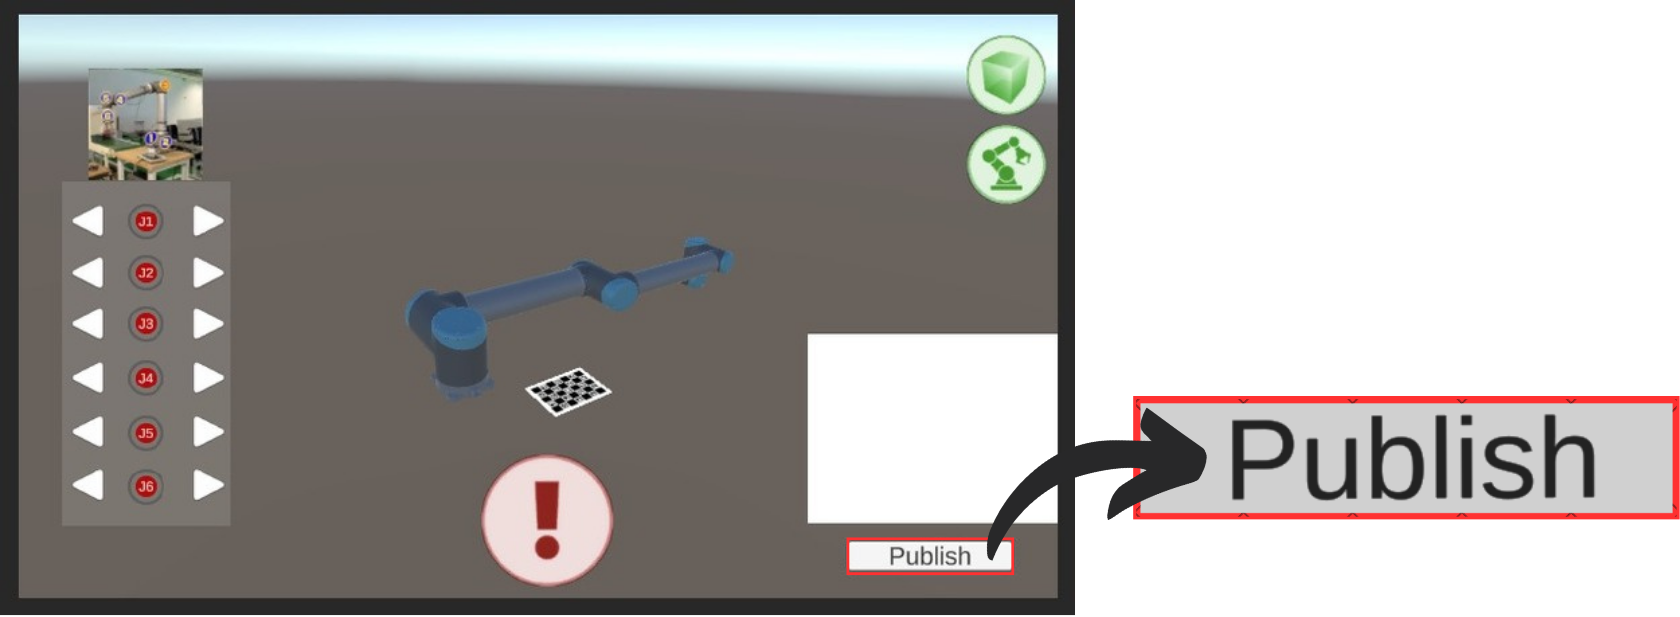
\includegraphics[width=0.8\linewidth]{figs/publish-button.png}
    \caption{Publish button that sends Unity's \ac{DT} robot joint states into ROS the environment}
    \label{fig:publish_UI_button}
\end{figure}

To avoid conflicts with the \ac{ROS} node responsible for controlling the real robot's joints, which are being constantly published to the standard \texttt{/joint\_states} topic, a separate \ac{ROS} topic \texttt{(/unity\_joint\_states)} was created to handle the joint data coming from Unity. This ensures that data from Unity does not interfere with the real robot’s ongoing operations. When the "Publish" button is pressed, the Unity-defined joint states are sent to this new topic, and only when necessary are they relayed to the real robot for movement execution. Algorithm \ref{alg:unity_input} represents a pseudo-code snippet that explains how to update the \ac{DT} in Unity and send the new desired robot position to the \ac{ROS} middleware.

\begin{algorithm}
    \caption{Unity Input for Joint Selection and Movement}\label{alg:unity_input}
    \begin{algorithmic}[1]
        \State \textbf{Step 1: User Input for Joint Selection and Movement in Unity}
        \While{Unity Simulation is running AND Unity-ROS Control is enabled}
            \If{RightArrowKeyPressed}
                \State Select next joint
            \ElsIf{LeftArrowKeyPressed}
                \State Select previous joint
            \EndIf
            \If{UpArrowKeyPressed}
                \State Rotate selected joint in positive direction
            \ElsIf{DownArrowKeyPressed}
                \State Rotate selected joint in negative direction
            \EndIf
            \If{PublishButtonPressed}
                \State joint\_states = GetCurrentJointStates()
                \State PublishToROSTopic(/unity\_joint\_states, /joint\_states)
            \EndIf
        \EndWhile
    \end{algorithmic}
\end{algorithm}


In order to handle this communication process, two new \ac{ROS} nodes were created, \texttt{joint\_state\_listener} and \texttt{move\_unity}. The \texttt{unity\_joint\_subscriber.py} script was developed within the \texttt{iris\_ur10e} package, initializing the node that subscribes to the \texttt{/unity\_joint\_states} topic, which receives a JointState message type. It then starts the publisher for the \texttt{/move\_joint\_unity} topic, converting this data into a Float64MultiArray format which will be further received by the second node. This second node called \texttt{move\_unity}, created within the \texttt{iris\_sami} package, subscribes to the \texttt{/move\_joint\_unity} topic, listening to new joint position values, moving the robotic arm to this desired position. This real-time update can be visualized either on the simulation environment, through Rviz, or by utilizing the real UR10e robot. Another pseudo-code algorithm explanation regarding how both \ac{ROS} nodes work, is presented in \ref{alg:combined_ros_node}.

% Part 2: ROS Node for Receiving Unity Joint States

\begin{algorithm}
    \caption{Combined ROS Node for Receiving Unity Joint States and Moving the Robot}\label{alg:combined_ros_node}
    \begin{algorithmic}[1]
        \State \textbf{Step 2 and 3: Combined ROS Node for Receiving Unity Joint States and Moving the Robot}
        
        \State Initialize ROS Node: joint\_state\_listener
        \State Subscribe to Topic: '/unity\_joint\_states'
        
        \While{Receiving JointState message from Unity}
            \State float\_array\_data = ConvertToFloat64MultiArray(joint\_states)
            \State PublishToROSTopic('move\_joint\_unity', float\_array\_data)
        \EndWhile
        
        \State \textbf{Precondition:} The \texttt{joint\_state\_listener} node must be running and publishing to the \texttt{'/move\_joint\_unity'} topic.
        \State Initialize ROS Node: test\_arm\_movement
        \State Subscribe to Topic: '/move\_joint\_unity'
        
        \While{Receiving Float64MultiArray message from \texttt{move\_joint\_unity}}
            \State MoveRobotArmTo(joint\_positions)
            \If{ConnectedToRealRobot}
                \State MoveRealRobot()
            \Else
                \State VisualizeInRviz()
            \EndIf
        \EndWhile
    \end{algorithmic}
\end{algorithm}


    
\subsection{Robot to Unity}

Opposite to the above described method which controlls the \ac{DT} and then updates the robot position, in this control method, the on-site user moves the robot and the remote counterpart visualizes this update instantly within the \ac{MR} environment.

In order to properly achieve this communication and data transfer, the \texttt{JointStateSubscriber.cs} script was created in Unity. It subscribes to the \texttt{/joint\_states} topic, and stores the information regarding the joint positions in a dictionary structure that is updated in real time into a specific \texttt{.json} file within the \ac{MR} environment. This file is constantly being read by the \texttt{Controller.cs} script whenever this control method is enabled, updating the \ac{DT} robot model accordingly.

By maintaining this synchronization between the real robot and the virtual environment, the Unity scene accurately reflects the robot's live state, ensuring a consistent \ac{DT} representation through the bidirectional communication established between the \ac{MR} environment and the \ac{ROS} middleware. Below, algorithm \ref{alg:ros_unity_control} explains how this \ac{ROS}-Unity control method works.


\begin{algorithm}
    \caption{ROS-Unity Control via Joint States Subscription}\label{alg:ros_unity_control}
    \begin{algorithmic}[1]
        \State \textbf{Step 1: Subscribe to ROS \texttt{/joint\_states} topic}
        \State Attach the Unity Script to the Digital Robot Model Asset: \texttt{JointStateSubscriber.cs}
        \State Upon Initialization, it subscribes to topic: \texttt{/joint\_states}

        \While{Receiving JointState message from \ac{ROS}}
            \State Extract joint names and positions from the message and store them in a dictionary data structure
            % \State Store them in a dictionary structure
            \State Save the dictionary data to the \texttt{jointStateSubscriber.json}
        \EndWhile

        \State \textbf{Step 2: Update Unity \ac{DT} Robot Model}
        \While{Simulation is Running}
            \State Read the \texttt{jointStateSubscriber.json}
            \State Update the Unity \ac{DT} robot model using the joint positions from the dictionary structure
        \EndWhile

        \State \textbf{Step 3: Synchronize Real Robot with \ac{DT} Robot}
        \State The Unity \ac{DT} robot model moves according to the real robot’s joint positions, ensuring a consistent bidirectional \ac{DT} representation.
    \end{algorithmic}
\end{algorithm}

Figure~\ref{fig:robot-unity} illustrates this real-time synchronization between the UR10e robot and its \ac{DT} within the \ac{MR} environment. As the on-site user manipulates the physical robot, its digital counterpart updates instantly within Unity, providing the remote user with a synchronized visual representation of the robot’s movements.

\begin{figure}[h]
    \centering
    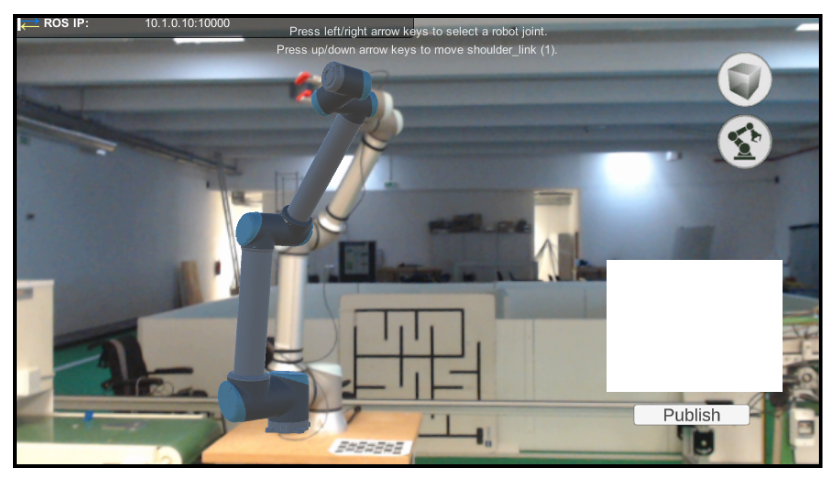
\includegraphics[width=\linewidth]{figs/super-imposed-robot.png}
    \caption{Real-time synchronization of the UR10e robot’s \ac{DT} in Unity environment, showing an overlay of the robot. This synchronization enables remote users to monitor the robot's state within the \ac{MR} environment, reflecting live updates via bidirectional \ac{ROS}-Unity communication}
    \label{fig:robot-unity}
\end{figure}


\section{Mixed-Reality Features}
\label{section:on-site-features}
% \input{chapters/on-site/on-site-features} commented this part because text is below - choose whether to use this or the text below
After having implemented the \ac{DT}-Robot bidirectional communication between the on-site and remote members, the next step consisted on developing features that could enhance both users' experience when interacting with the collaboration environment. These features were designed to improve user safety, facilitate robot manipulation, and provide an intuitive interface. The following sections detail these key features development and implementation.

% Regarding the on-site member's collaboration experience, as explained in the state of art review, by implementing different sensorial cues, such as visual and audio, it will enhance the user experience into a more intuitive and immersive way.

\subsection{Virtual Safety Zones and Sensorial Cues}
\label{subsection:virtual-safety-zones} 
% \input{chapters/on-site/subsections/virtual-safety-zones} commented this part because text is below - choose whether to use this or the text below

As explained in section \ref{sec:hrc-in-industry}, introducing different sensorial cues enhances on-site users' experience into a more intuitive and immersive experience. Therefore, visualizing the working zone of the robot is a critical feature designed to enhance safety when interacting with the robot. Figure \ref{fig:safety-zones} displays the developed safety-zones that aim to increase awareness around the robot's working space. Alongside these two safety zones' development, other features that address specific safety and user's concerns are explained below:  

\begin{figure}[h]
    \centering
    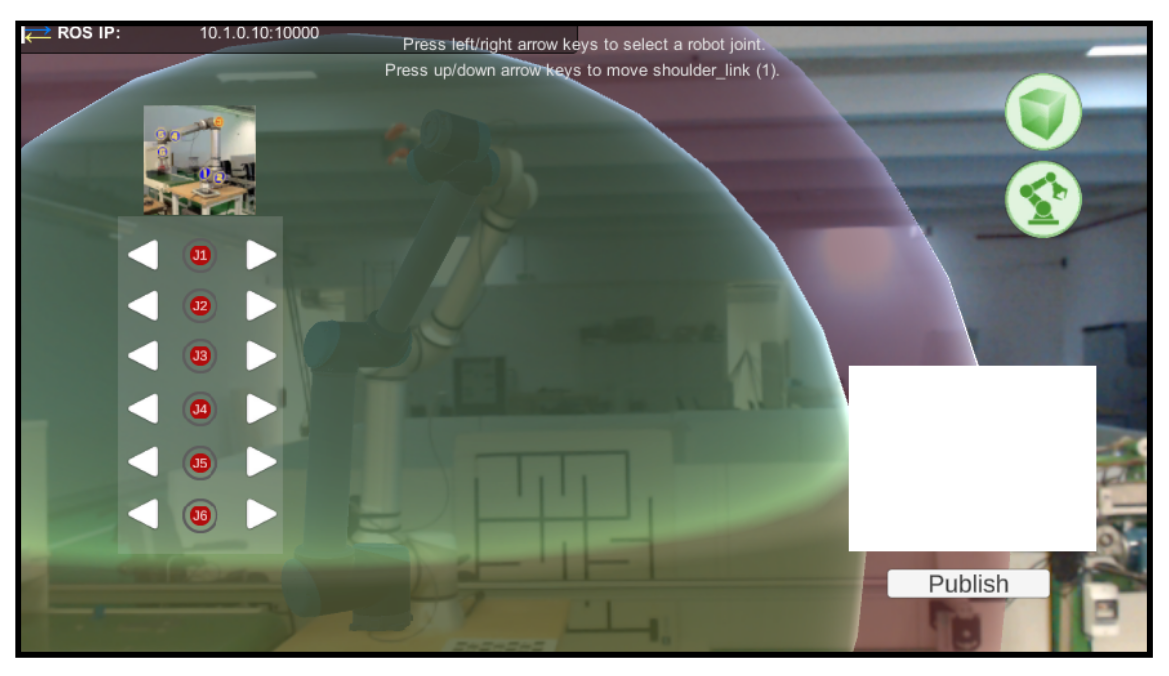
\includegraphics[width=\linewidth]{figs/safet-zones.png}
    \caption{\ac{MR} application \ac{UI}, with safety-zones aumenting the robot's working area in order to address user's safety}
    \label{fig:safety-zones}
\end{figure}

\begin{itemize}
\item \textbf{Outer Safety Zone:} Initially, only this safety zone was created. The purpose of creating it was to provide an 
early warning to users as they approach the hazardous area near the robot. This approach consisted on changing its color as a visual alert. 
However, this method proved ineffective because, once inside it, users could not perceive the color change, rendering the warning system inadequate.

\item \textbf{Inner Safety Zone:} To overcome this outer zone limitation, an additional Inner-Safety Zone was developed. This design ensures a two-step safety mechanism that properly alerts users when they are in close proximity to the robot.

\item \textbf{Sensorial Cues: } Feedback was provided using distinct sensorial cues, namely:
\begin{itemize}

    \item \textbf{Visual}: Upon entering the Outer-Safety Zone, the color of the Inner sphere changes to red, reverting to its default color if the user exits this critical area. This visual cue alerts the user to increased proximity to a high-risk zone. Additionally, a blinking warning appears at the bottom center of the interface, switching between both circular danger signs shown in Figure \ref{fig:blinking-sign}. This flashing indicator amplifies the alert, reinforcing the awareness of approaching the operational robot area, remaining active as long as the user is within this Outer-Safety Zone.

    \item \textbf{Auditory}: Entering the Inner-Safety Zone triggers an audio alarm signifying that the user has breached into the robot working area, enhancing the effectiveness of the safety mechanism.
\end{itemize}

\begin{figure}[h]
    \centering
    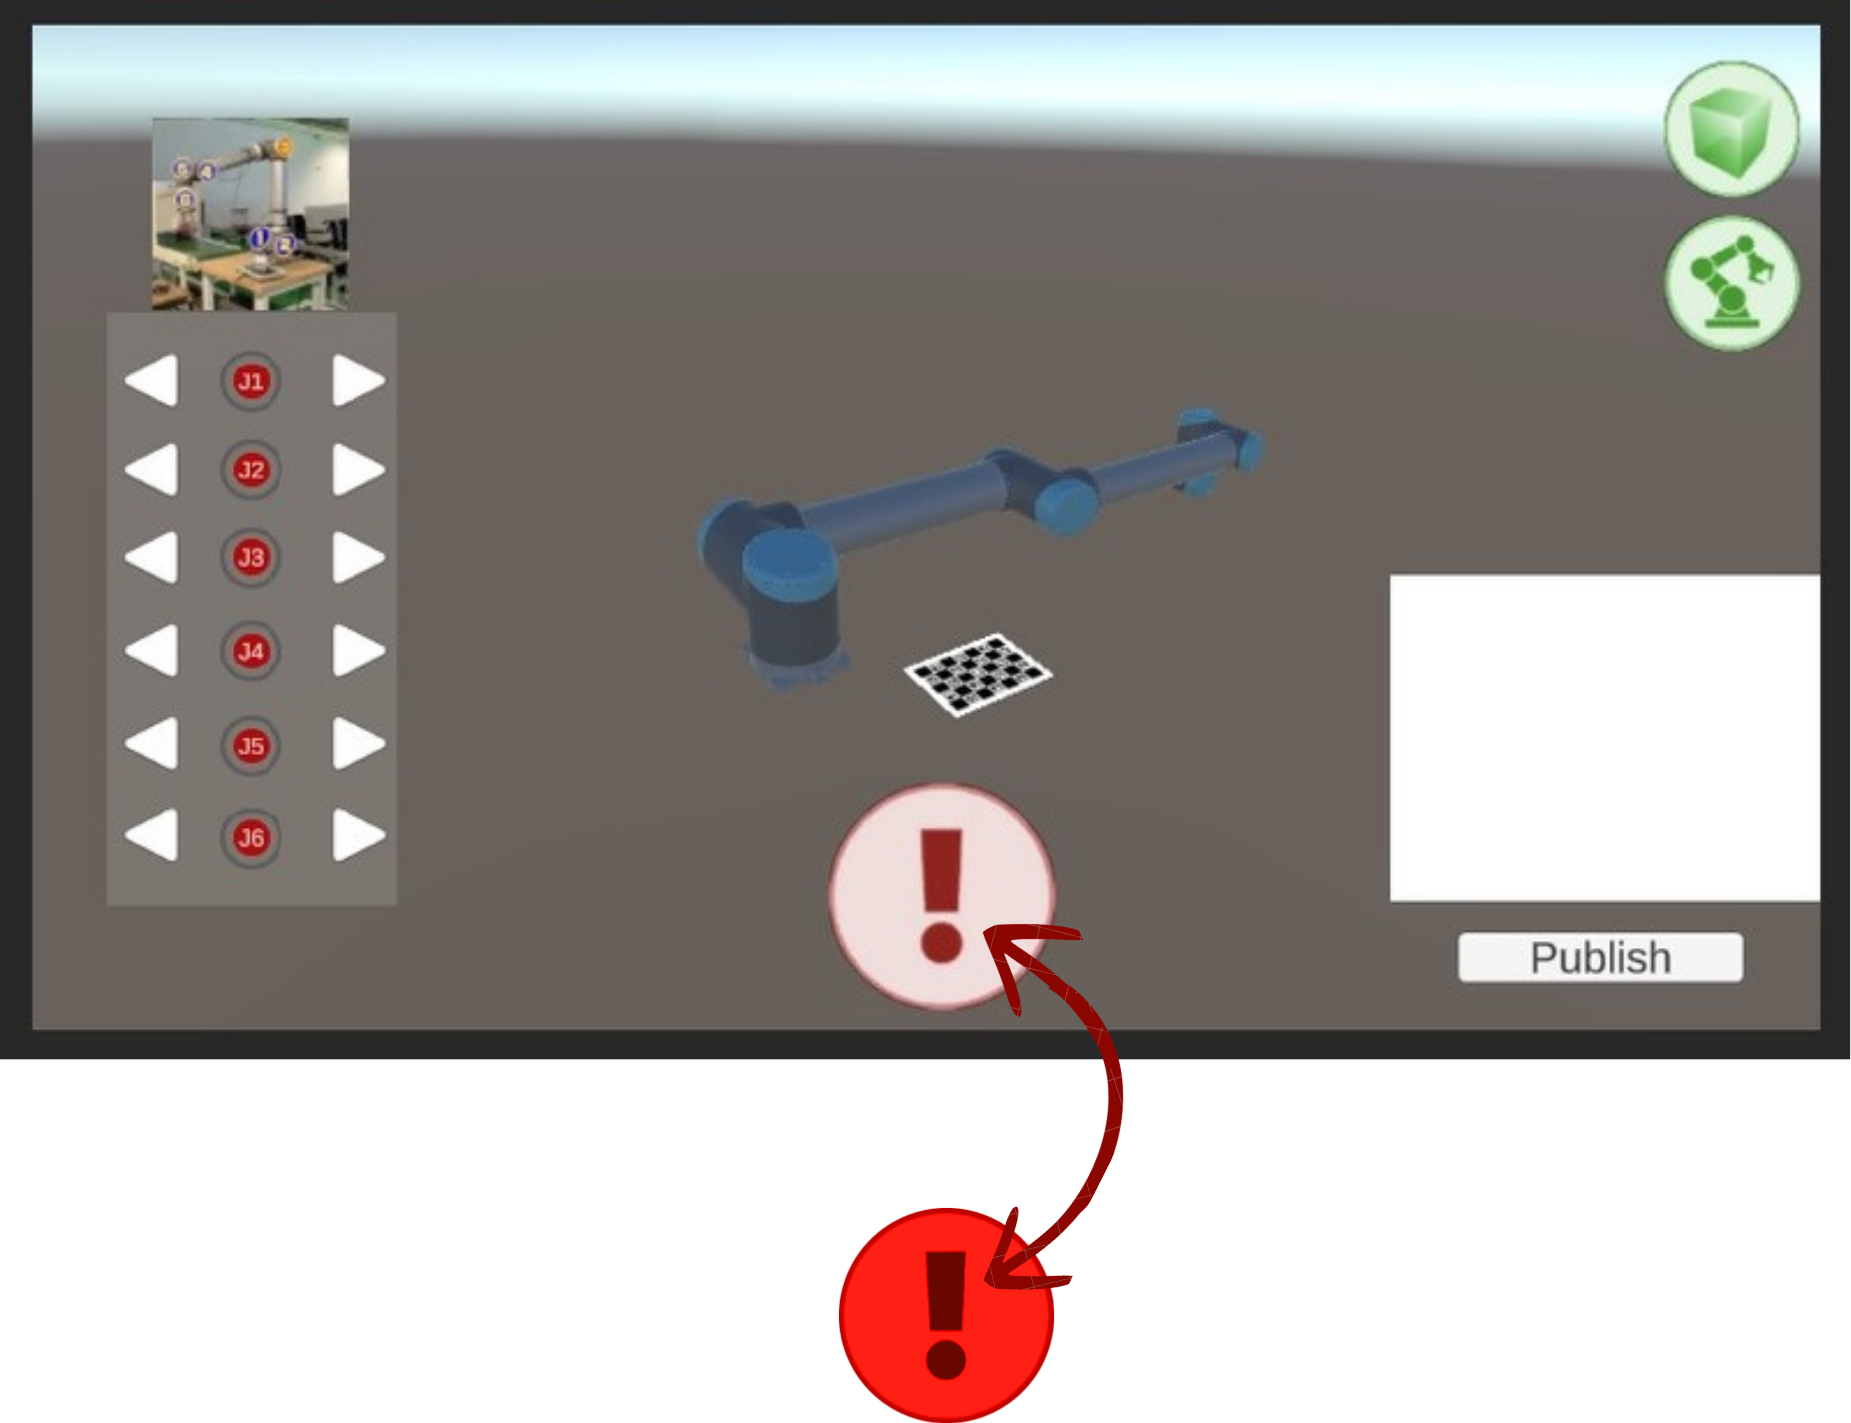
\includegraphics[width=0.7\linewidth]{figs/sign-alert.png}
    \caption{Warning blinking sign displayed in the bottom part of the \ac{UI} to alert the on-site user of proximity to the Robot}
    \label{fig:blinking-sign}
\end{figure}

\item \textbf{Breach Protocol:} Besides the above described sensorial cues whose goal consists on improving user's awareness, another feature was implemented to ensure user's safety when interacting with the robot. If the on-site counterpart enters the Outer-Safety Zone while the robot is in motion, the robot automatically stops. This immediate halt ensures that potential accidents or injuries are avoided by preventing any interaction with the robot when a user is within this designated dangerous area.
\end{itemize}
    
% this interface section - the feature of controlling it using the UI must be put in the UI COntrol method above
%  the remaining part should be in this part - explaining the rest of the UI features
\subsection{Flexible Interface Options for User Customization}

Additional features were integrated into the \ac{MR} application aimed at enhancing user flexibility and clarity. Positioned in the upper right corner of the \ac{UI}, two green toggle buttons provide control over distinct interface functionalities. By utilizing these two toggle buttons, users can enable/disable the visibility of both safety zones and the robot joint control panel for an optimized workspace view. 

% \begin{figure}[h]
%     \centering
%     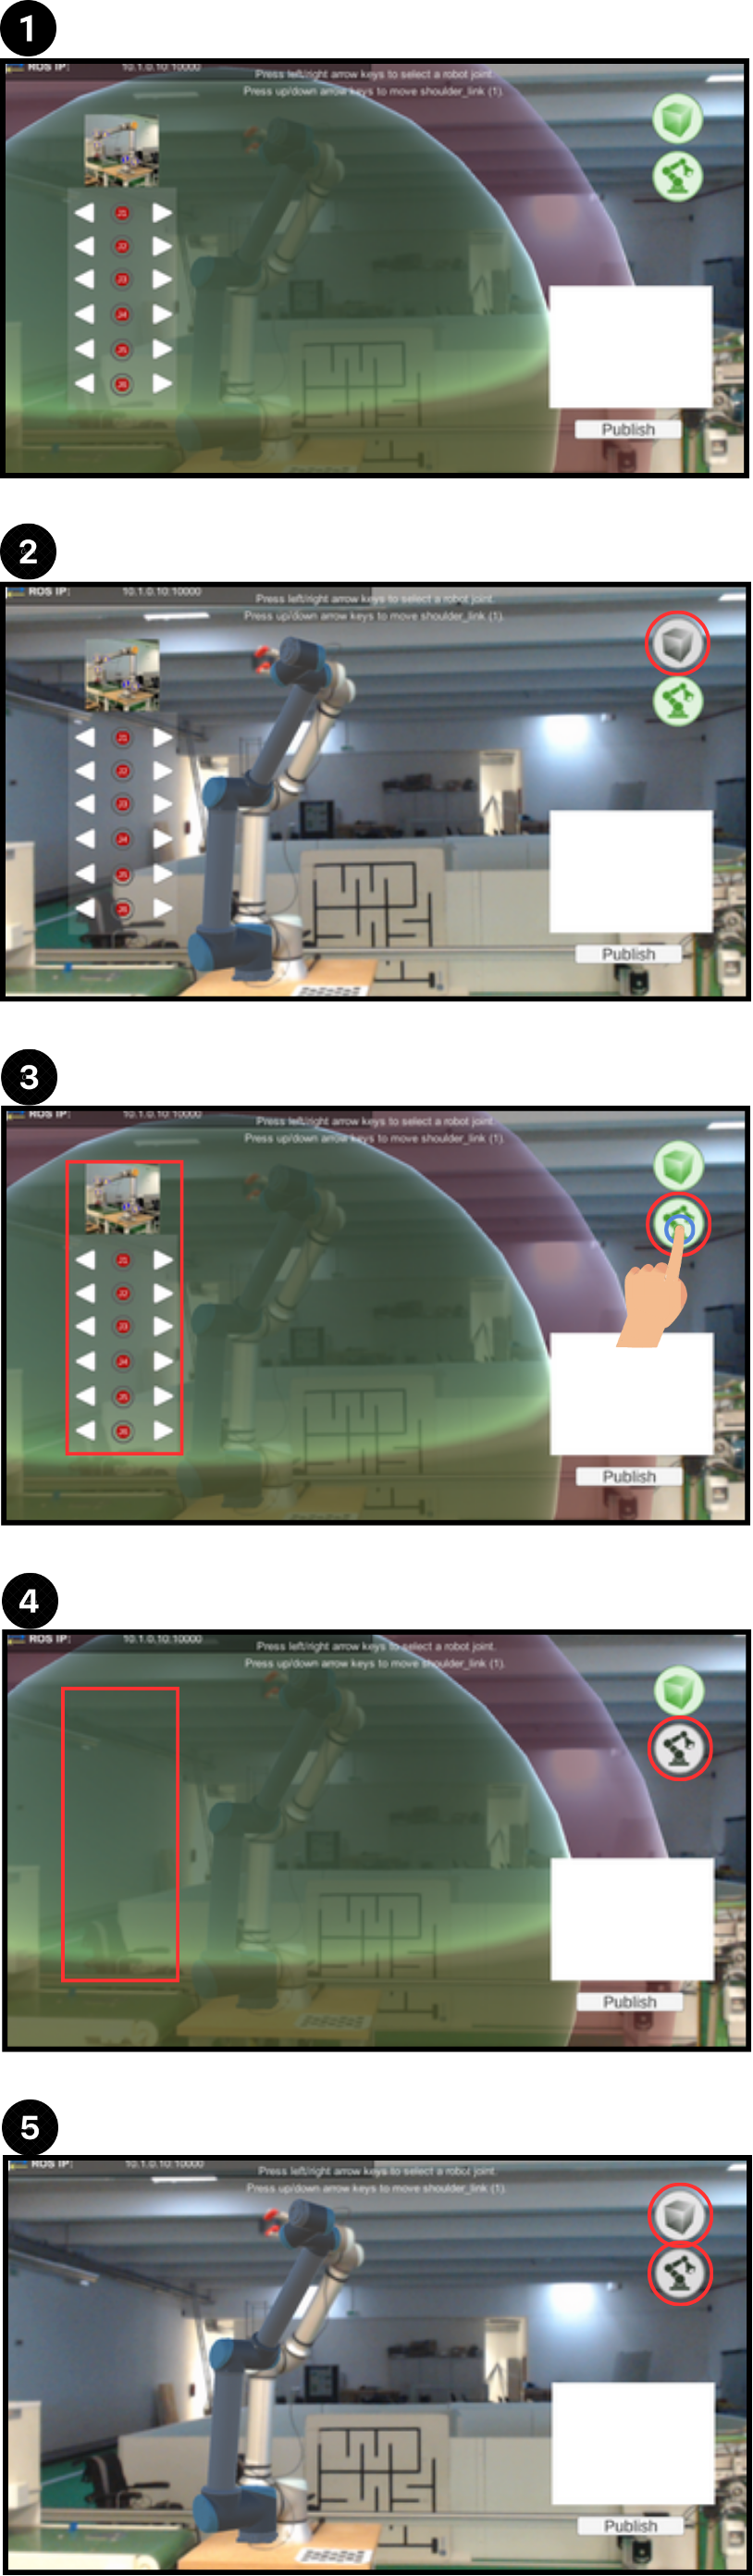
\includegraphics[width=\linewidth]{figs/all-features-3.png}
%     \caption{\ac{UI} demonstrating the activation and deactivation of the safety zones and robot joint control panel within the \ac{MR} environment. In (1), the workspace is displayed with the safety zones active. By pressing the top-right button in (2), these zones are deactivated, providing a clearer view. In (3), pressing the button below the top-right icon deactivates the joint control panel, as seen in (4). In (5), with both buttons deactivated, the workspace is entirely unobstructed, offering maximum clarity for the user}
%     \label{fig:all-features-button}
% \end{figure}

Figure \ref{fig:safety-zones-button} represents this \ac{MR} interface flexibility. In image \ref{fig:subfig1}, both safety zones and control panels are active. By selecting the upper-right button, the user can deactivate safety zones, turning this toggle button into gray and thus, removing visual cues and safety-zones related features. This deactivation is depicted in \ref{fig:subfig2}, where a clearer view of the environment can be visualized.

\begin{figure}[h]
    \centering
    % First subfigure
    \begin{subfigure}{\textwidth}
        % \captionsetup{justification=raggedright, singlelinecheck=false, position=top}
        \caption{}
        \centering
        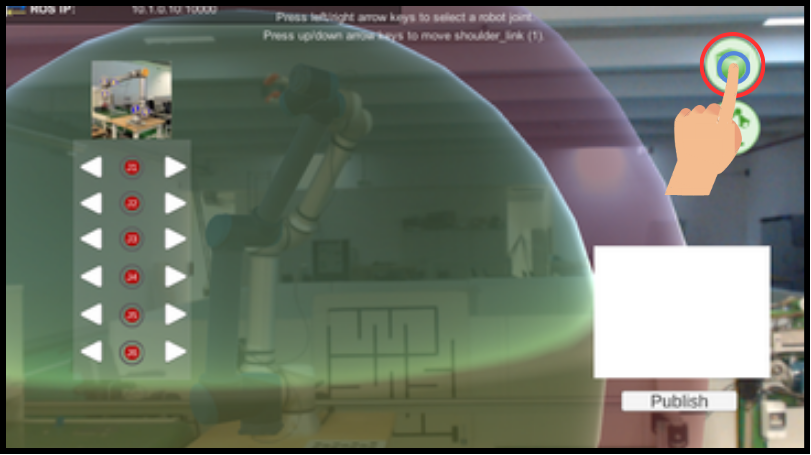
\includegraphics[width=0.7\textwidth]{figs/feature-1.png}
        % \caption{Both safety zones and control panel are active, providing full visual feedback. Upon pressing the upper-right toggle button, safety-zones are disabled.}
    \label{fig:subfig1}
    \end{subfigure}

    \vspace{0.5em} % Add space between figures

    % Second subfigure
    \begin{subfigure}{\textwidth}
        % \captionsetup{justification=raggedright, singlelinecheck=false, position=top}
        \caption{}
        \centering
        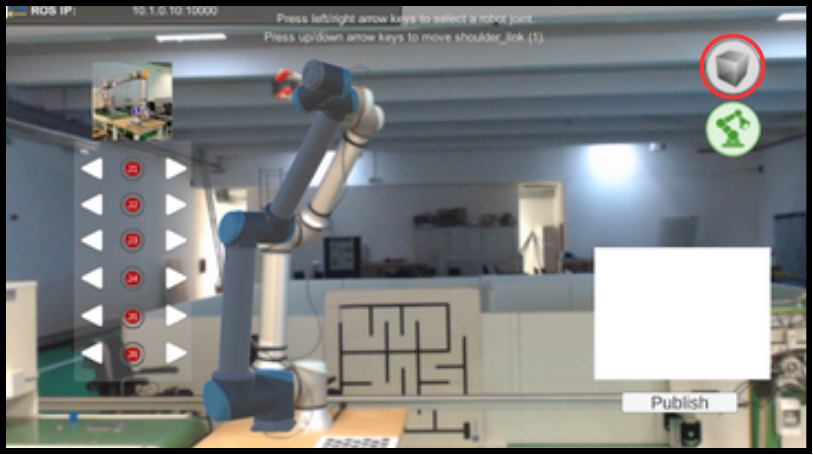
\includegraphics[width=0.7\textwidth]{figs/feature-2.png}
        % \caption{Consequence of pressing the upper-right toggle button, removing safety cues and providing a clearer view.}
        \label{fig:subfig2}
    \end{subfigure}
    \caption{Flexible \ac{MR} interface for activating and deactivating safety zones. In subfigure \ref{fig:subfig1}, both safety zones are active, providing visual cues for the user. By selecting the top-right toggle button, subfigure \ref{fig:subfig2} shows the deactivated state of the safety zones, removing these visual elements to enable an unobstructed workspace view.}
    \label{fig:safety-zones-button}
\end{figure}

Regarding the joint control panel used to manipulate the robot through the interface, an activation/deactivation toggle was also added to the \ac{UI}. This interaction is displayed in Figure \ref{fig:3-features-button} where it is clear that by pressing the lower button represented in \ref{fig:subfig3}, the joint control panel is removed from the \ac{MR} environment. This toggle also behaves in the same way of the one from \ref{fig:subfig1}, turning into gray upon deactivation. 
Finally, Figure \ref{fig:subfig5} represents the deactivation of both features, achieving an unobstructed view. These customization options allow users to adjust the interface according to task requirements, balancing between safety feedback and workspace clarity.


% The lower button, pressed in image \ref{fig:subfig3}, toggles the robot joint control panel on and off, as illustrated in image \ref{fig:subfig4}. This toggle also behaves in the same way of the above one, turning into gray upon deactivation. Image \ref{fig:subfig5} represents the deactivation of both features, achieving an unobstructed view. These customization options allow users to adjust the interface according to task requirements, balancing between safety feedback and workspace clarity.

% Figure \ref{fig:all-features-button} demonstrates this \ac{MR} interface flexibility. In image \ref{fig:subfig1}, both safety zones and control panels are active. By selecting the upper-right button, the user can deactivate safety zones, turning this toggle button into gray and thus, removing visual cues and safety-zones related features, as depicted in \ref{fig:subfig2}. The lower button, pressed in image \ref{fig:subfig3}, toggles the robot joint control panel on and off, as illustrated in image \ref{fig:subfig4}. This toggle also behaves in the same way of the above one, turning into gray upon deactivation. Image \ref{fig:subfig5} represents the deactivation of both features, achieving an unobstructed view. These customization options allow users to adjust the interface according to task requirements, balancing between safety feedback and workspace clarity.


\begin{figure}[h]
    % Third subfigure
    \begin{subfigure}{\textwidth}
        % \captionsetup{justification=raggedright, singlelinecheck=false, position=top}
        \caption{}
        \centering
        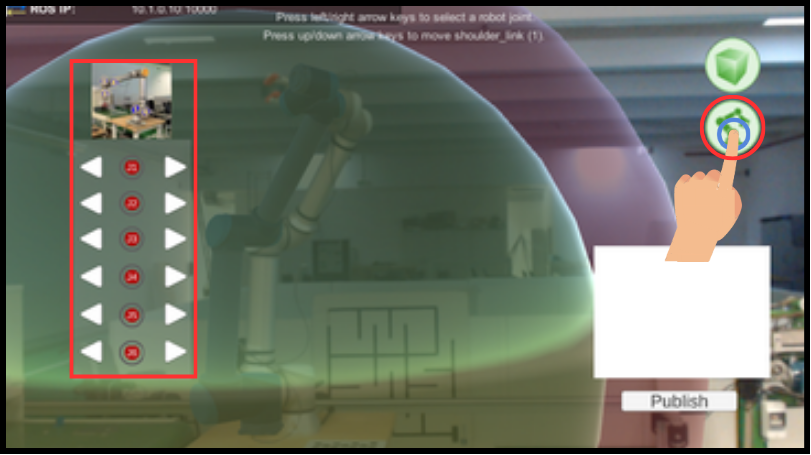
\includegraphics[width=0.7\textwidth]{figs/feature-3.png}
        % \caption{Pressing of the lower-right toggle button to deactivate the robot joint control panel.        
        \label{fig:subfig3}
    \end{subfigure}

    \vspace{0.5em}

    % Fourth subfigure
    \begin{subfigure}{\textwidth}
        % \captionsetup{justification=raggedright, singlelinecheck=false, position=top}
        \caption{}
        \centering
        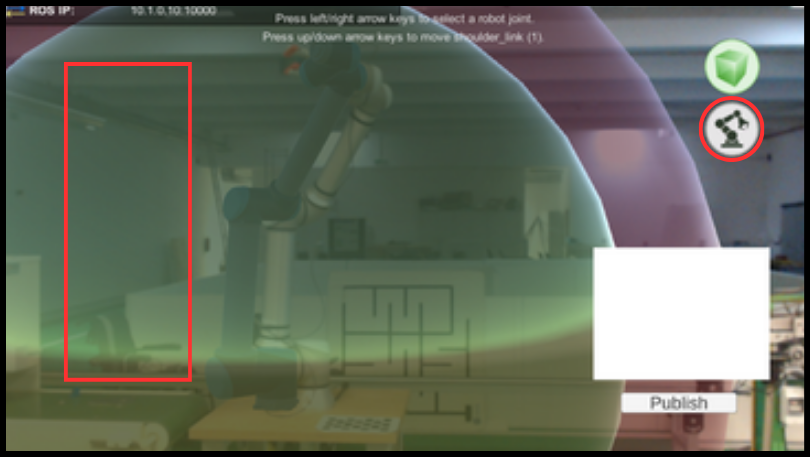
\includegraphics[width=0.7\textwidth]{figs/feature-4.png}
        % \caption{Robot joint control panel deactivated, allowing a more streamlined interface.}
        \label{fig:subfig4}
    \end{subfigure}

    \vspace{0.5em}

    % Fifth subfigure
    \begin{subfigure}{\textwidth}
        % \captionsetup{justification=raggedright, singlelinecheck=false, position=top}
        \caption{}
        \centering
        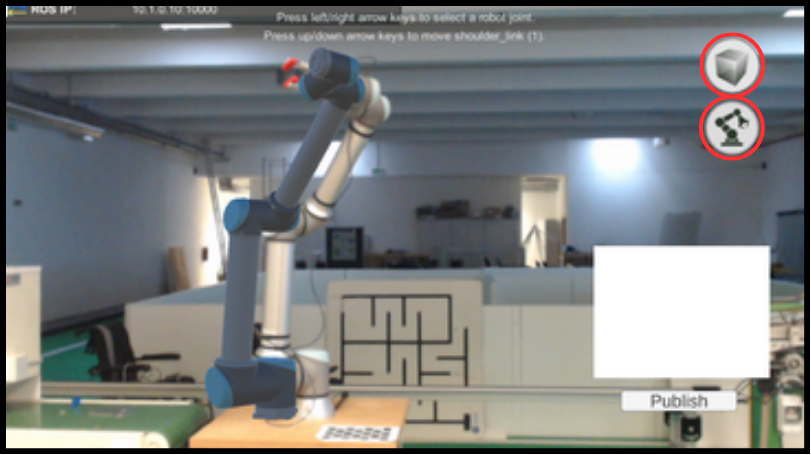
\includegraphics[width=0.7\textwidth]{figs/feature-5.png}
        % \caption{Both safety zones and control panel are deactivated, achieving an unobstructed workspace view.}
        \label{fig:subfig5}
    \end{subfigure}

    \caption{Flexible \ac{MR} interface options for robot joint control panel management. Subfigure \ref{fig:subfig3} displays the joint control panel active, allowing users to manipulate the robot’s joints. Upon pressing the lower toggle button, subfigure \ref{fig:subfig4} shows the deactivation of this control panel, creating a less cluttered interface. In subfigure \ref{fig:subfig5}, both the safety zones and control panel are deactivated, offering a fully unobstructed view of the workspace for optimal clarity.}
    \label{fig:3-features-button}
\end{figure}



\subsection{Enhanced Remote Visualization Through Camera Feed Transmission}

To improve situational awareness for remote users, an additional camera was integrated, providing real-time visual context directly from the robot’s perspective and reducing on-site operator's responsibility for managing environmental views.
% *TODO: check this, it was mounted on top of the robot (?-lie)
The Orbbec Astra 3D camera~\footnote{\url{https://www.orbbec.com/products/structured-light-camera/astra-series/} Acessed:2024-10-22}, shown in Figure \ref{fig:astra-camera}, was chosen for its compatibility with the \ac{ROS} framework. This camera was mounted directly onto the robot, offering an immersive view that aligns with the robot’s operational perspective. Integration into the \ac{ROS} environment was facilitated through the Astra camera’s dedicated GitHub repository~\footnote{\url{https://github.com/orbbec/ros\_astra\_camera} Accessed: 2024-10-04}, which provided essential drivers and nodes for \ac{ROS} compatibility.

\begin{figure}[h]
    \centering
    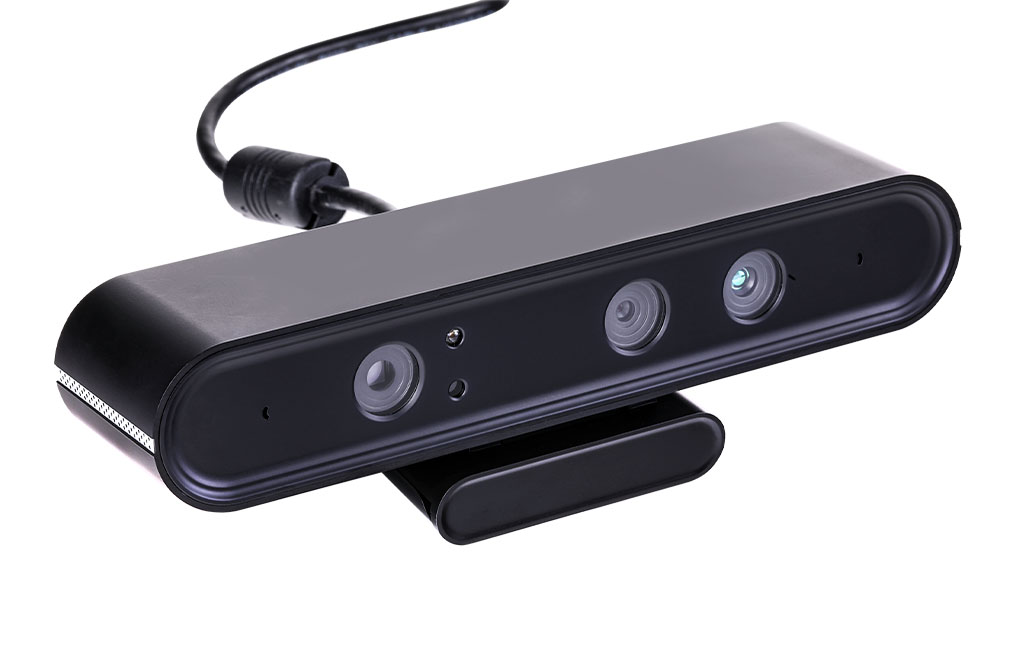
\includegraphics[width=0.5\linewidth]{figs/AstraSeries_3.jpg}
    \caption{Orbbec Astra 3D camera mounted on the UR10e robotic arm, providing a real-time visual feed of the robot's environment to support remote user awareness}
    \label{fig:astra-camera}
\end{figure}

The live feed from the Astra camera was managed via the \texttt{astra\_camera\_node} from the \texttt{astra\_camera} package, enabling continuous data capture and real-time display in RViz for preliminary verification. This configuration ensured proper camera functionality within the \ac{ROS} environment and accurate data capture. 

However, when transmitting the uncompressed image data to the Unity \ac{MR} application, bandwidth and latency challenges arose, potentially impacting real-time collaboration. To address this, the \ac{ROS} \texttt{image\_transport} package was used, which converted the raw video stream into a compressed format, reducing data size while preserving essential image quality. By compressing the image data, the system achieved more efficient and stable real-time transmission to Unity, providing continuous visual feedback with minimal latency. The following command facilitated the data compression:

\begin{verbatim} 
    rosrun image_transport republish raw in:=/camera/color/image_raw 
    out:=/camera/image_repub 
\end{verbatim}

Afterwards, this compressed camera feed had to be integrated into Unity. To do this, the \texttt{CameraFeedReceiver.cs} script was developed, responsible for receiving and rendering the feed into the \ac{UI} panel. This setup allowed the remote user to view the robot’s perspective in real time, independent of the on-site operator’s actions. This dual-view capability offers the remote user a comprehensive visual overview by combining the on-site provided view with the camera feed directly from the robot’s perspective, potentially enhancing spatial awareness and operational context.

Figure \ref{fig:camera-feed} demonstrates the live feed display in Unity, showcasing how the system allows remote users to monitor the robot’s surroundings and adjust their commands accordingly. This feature may support more informed decision-making in future implementations of remote \ac{MR} systems for \ac{HRC}.

% \begin{figure}[h]
%     \centering
%     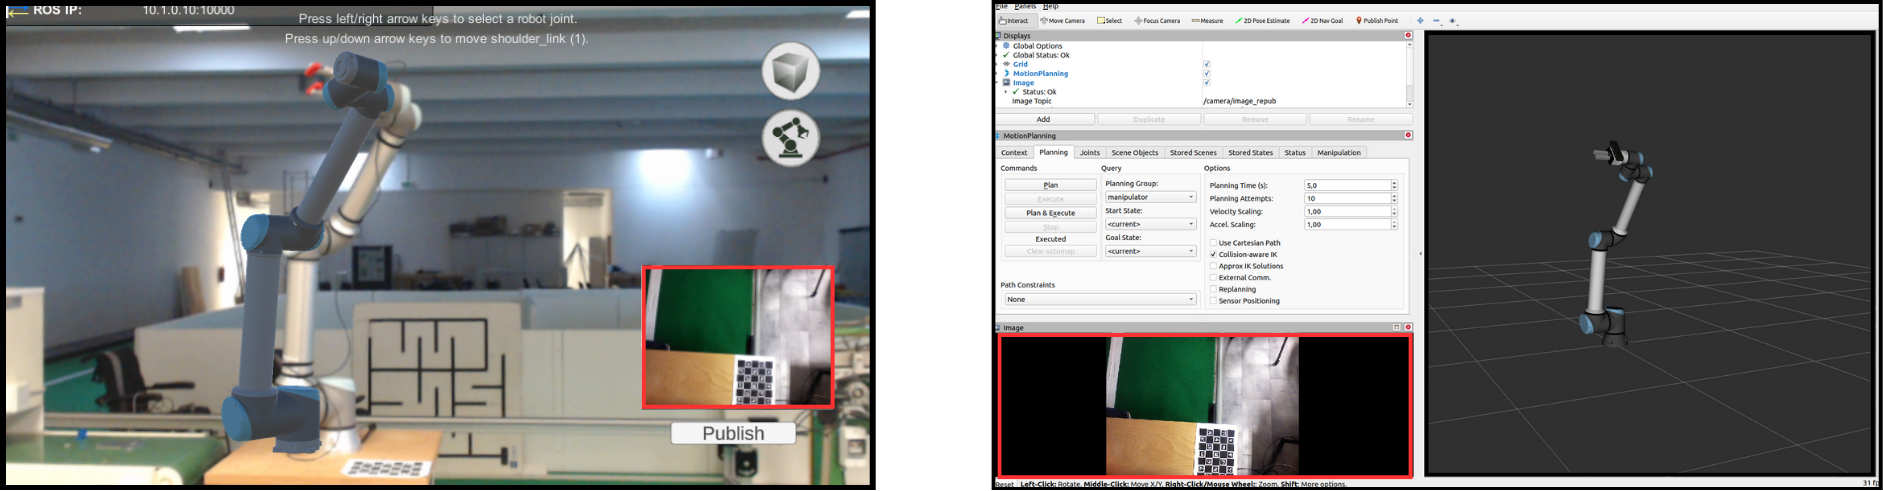
\includegraphics[width=\linewidth]{figs/camera-feed-transmission-3.png}
%     \caption{Real-time camera feed integration from the robot’s perspective within the \ac{MR} environment. On the left image, Unity displays the \ac{MR} interface seen by the remote user, with emphasis on the live feed coming from the camera mounted on the robot, aiming to enhance situational awareness. The right picture shows the RViz simulation where the camera feed is captured through the \ac{ROS} Middleware setup. This live camera transmission between on-site and remote users has to be compressed, ensuring the proper quality and minimal latency between environments, enabling synchronized visualization.}
%     \label{fig:camera-feed}
% \end{figure}

\begin{figure}[h]
    \centering
    % First subfigure
    \begin{subfigure}{\textwidth}
        \centering
        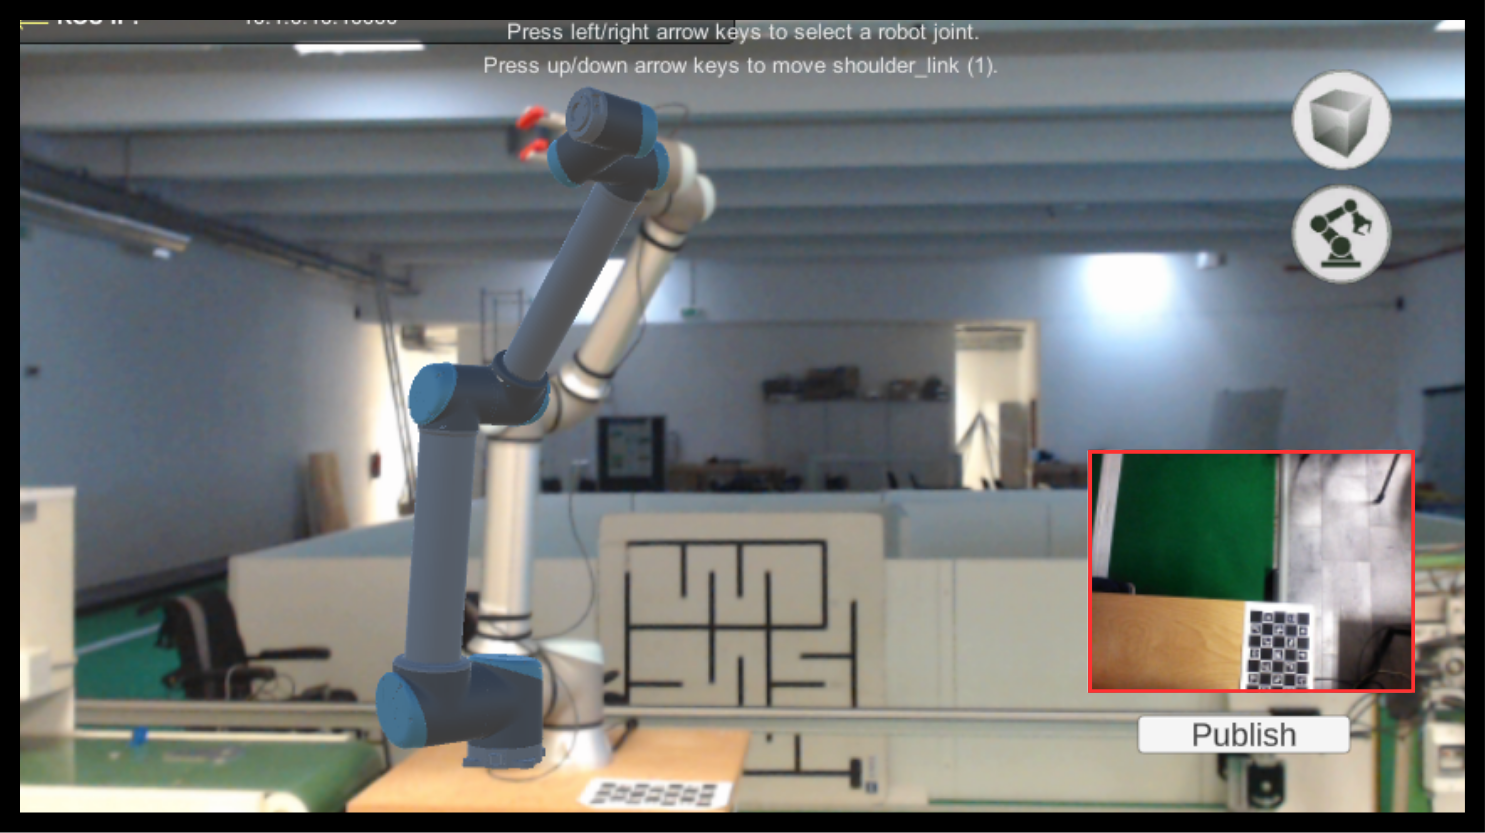
\includegraphics[width=0.75\textwidth]{figs/camera-feed-transmission-alone-1.png}
        \caption{Unity \ac{MR} environment displaying the robot’s camera feed, providing the remote user with real-time situational awareness of the robot’s workspace.}       
        \label{fig:camera-unity}
    \end{subfigure}

    \vspace{0.8em} % Add space between figures

    % Second subfigure
    \begin{subfigure}{\textwidth}
        \centering
        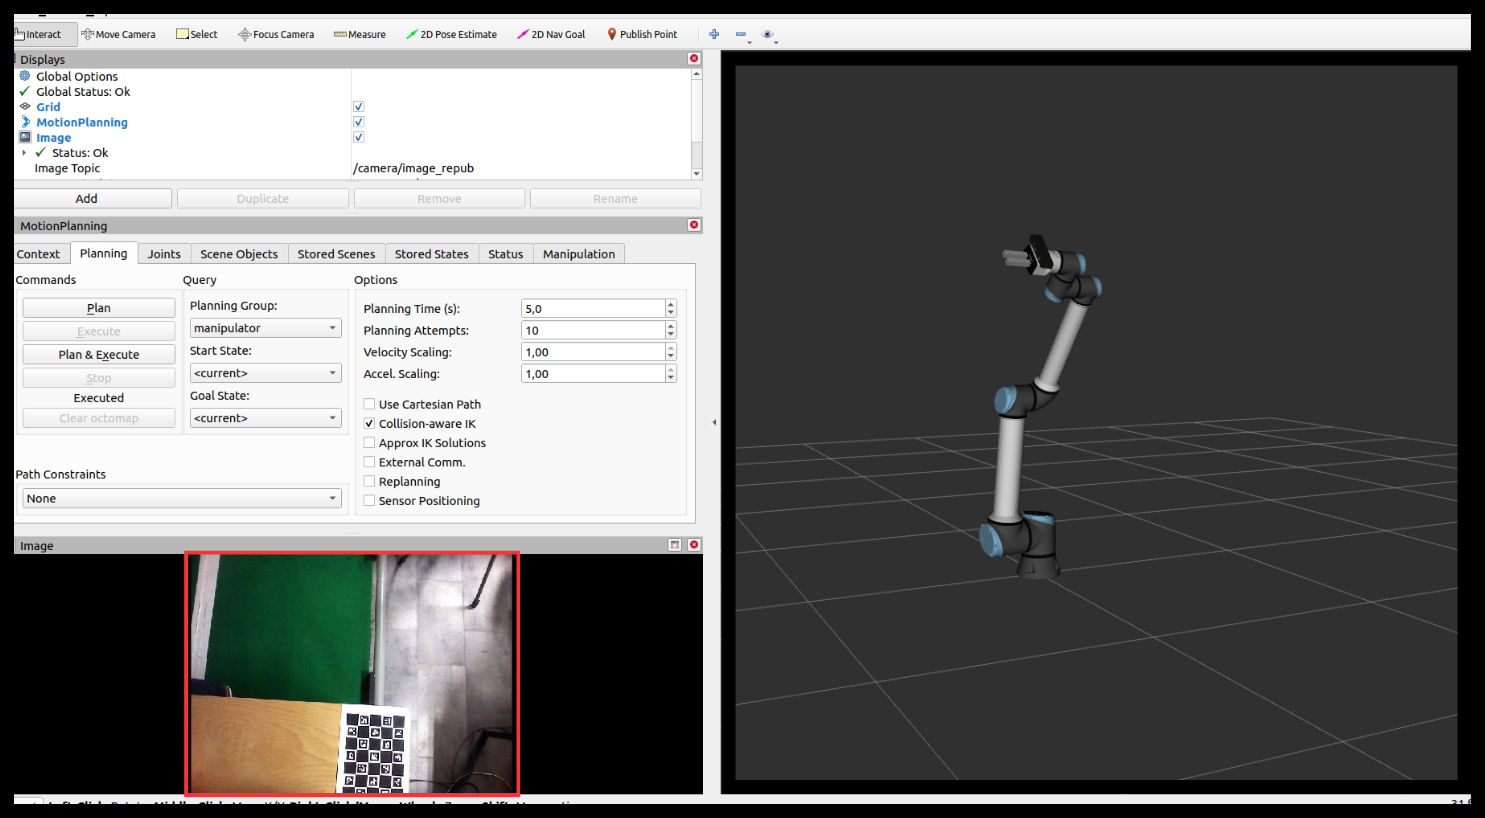
\includegraphics[width=0.75\textwidth]{figs/camera-feed-transmission-alone-2.png}
        \caption{RViz interface showing the camera feed integrated through \ac{ROS}, used for verifying the robot’s field of view and validating alignment with the \ac{MR} display in Unity.}
        \label{fig:camera-rviz}
    \end{subfigure}
    
    \caption{Real-time camera feed integration from the robot’s perspective within the \ac{MR} environment. On \ref{fig:camera-unity}, Unity displays the \ac{MR} interface seen by the remote user, with emphasis on the live feed coming from the camera mounted on the robot, aiming to enhance situational awareness. The \ref{fig:camera-rviz} picture shows the RViz simulation where the camera feed is captured through the \ac{ROS} Middleware setup. This live camera transmission between on-site and remote users has to be compressed, ensuring the proper quality and minimal latency between environments, enabling synchronized visualization.}
\label{fig:camera-feed}
\end{figure}


% "how the system allows remote users to monitor the robot’s surroundings and adjust their commands accordingly" - this sentence means that it can visualize the robots working view and manipulate the robot to make informed decisions and move it to where it wants to.  





% To initiate the camera feed, the \texttt{astra\_camera\_node} from the \texttt{astra\_camera} package is initialized. Afterwards, an RVIZ image viewer displays the live feed, ensuring the camera is functioning correctly and capturing the desired video data.

% * TODO: add a picture of the UI showing that the camera live feed from Rviz
% * TODO: need to explain better how the image transmission is sent to the Unity, needed to compress the image data into a different format, from raw to compressed, to be able to send it over Wi-Fi - used the image\_transport package to republish the image data in a more efficient format, allowing for smoother and real-time transmission to the Unity environment.
% after launching the camera node, the image data was republished using the image\_transport package, which allowed for smoother and real-time transmission to the Unity environment.
% * TODO: reorganize this part better

% \subsection{Unity Camera Feed Integration}

% After the camera live feed was displayed in the Rviz simulation within the on-site environment, this data needs to be transmitted to the Unity \ac{MR} application, allowing the remote user to observe the robot's environment in real-time, providing critical visual feedback necessary for effective remote collaboration.


% From the Unity side, the \texttt{CameraFeedReceiver.cs} (verify the name of the script) script was developed to receive and display the live camera feed. This script was then atached to an UI interface (confirm the name of the element) that displayed the video feed in real-time. 
% add a figure of the UI interface with the view of the camera - The figure (add figure) illustrates the camera feed in the Unity application, showcasing the live video stream from the robot's environment.

% \subsection{Data Transmission to Unity} 
    
% However, the raw image data generated by the camera was too heavy to be transmitted efficiently over Wi-Fi, so this data needed to be republished using the \texttt{image\_transport} package.
% By utilizing the following \ac{ROS} command 
% \begin{verbatim}
%     rosrun image_transport republish raw 
%     in:=/camera/color/image_raw out:=/camera/image_repub
% \end{verbatim}
% the image data was republished in a more efficient format, allowing for smoother and real-time transmission to the Unity environment.



% *TODO: is this useful to any integration part of this chapter????  - from chapter 5 beginning
% One of the key features developed was a seamless control method integrated within the \ac{MR} environment, allowing the user to manipulate the robot via the \ac{UI}. This interface includes joint's selection buttons, directional controls, and toggle switches for precise manipulation of each robotic joint.  This setup enables users to control the robot's movements through the \ac{MR} interface and send this position update to the \ac{ROS} middleware, with real-time synchronization ensuring the robot accurately mirrors the \ac{DT}'s state.

% The development of two safety zones within the \ac{UI} was a critical enhancement aimed at ensuring user safety and improving operational awareness when interacting with the robot. These zones function by providing real-time alerts to the user. When the user enters the "Outer Safety Zone", which has a larger radius, not only a visual alert starts blinking, but also the color of the "Inner Safety Zone" changes, signaling that the user is approaching the robot's workspace. These visual cue escalate the user's awareness of proximity to the robot. If he gets even closer to the robot and breaches the "Inner Safety Zone", an auditory alarm is triggered, continuously alerting the user to their presence within a hazardous area. This layered approach—combining visual color changes and auditory alarms—ensures that users are fully aware of any potential danger during robot operation, thereby preventing accidents. Moreover, the combination of these sensorial cues also contributes to a more immersive interaction experience, increasing awareness without overwhelming the user.
% However, the accuracy of these safety zones is heavily dependent on the alignment between the camera and the \ac{AR} marker. Misalignment between the them can lead to inaccuracies in distance measurements, affecting the reliability of the safety zones. Maintaining precise marker tracking is therefore essential for ensuring both the accuracy of safety zone alerts and the overall safety of the system during operation.

% Another significant feature was the implementation of a live camera feed, allowing the remote participant to view the robot’s workspace in real-time. This feed is crucial for remote collaboration, enabling users from different locations to have a synchronized understanding of the robot’s surroundings. The camera feed is transmitted from the \ac{ROS} middleware to the Unity \ac{MR} environment via \ac{TCP}/\ac{IP} after image compression. Compression was necessary due to the substantial bandwidth required for raw video data transmission. This feature offers an important perspective for remote users, aiding in monitoring and providing assistance when necessary.

% Both the joint control interface and the safety-zone mechanisms were designed to be toggled on/off, thereby ensuring that the user has the option to clear the \ac{UI} for an unobstructed view of the environment.


\chapter{Discussion}
*TODO: por introducoes em todos os capitulos
*TODO: nao ha necessidade de constatar o que foi implementado de novo, porque isso ja esta no capitulo anterior.
por o caso de futura aplicacao neste capitulo, 1 ou 2
*TODO: reformulate how does it make sense, since there were no performed user tests, how should i say that no evaluation can be done, since the focus remained on implementing the interface and functionalities and not in perform user test cases - there was time for this

In this section, a critical discussion of the developed \ac{MR} environment will be done, regarding this dissertation's objectives.

\section{Mixed Reality reflection on the proposed framework}

\subsection{Challenges and Issues Faced}
%  continue here
Though the development of these functionalities was successful, several challenges were encountered during the implementation phase that required substantial effort. The first hurdle was the integration of the robot’s digital model into the Unity environment using the Unity Robotics Hub's \texttt{URDF Importer} package. Unfortunately, an exact UR10e model was not available on-line, and a UR10 model was used instead \footnote{PositronicsLab \url{https://github.com/PositronicsLab/reveal_packages/tree/master/industrial_arm/scenario/models/urdf/ur10} Accessed: 2024-02-05}. This change did not pose any significant problem, as the physical properties and kinematics between the two models are the same, allowing for accurate simulation.

Ensuring accurate pose registration and alignment between the physical robot and its \ac{DT} in Unity presented a challenge. This required using a marker for precise \ac{AR} visualization. After testing several methods, an ArUco marker proved most effective for reliable tracking and better model alignment. Implementing this through Vuforia \ac{SDK} within Unity, along with relative positioning between the marker and digital model, was essential for maintaining synchronization between the physical and digital entities. However, practical issues arose during testing, as the camera and laptop needed to be moved frequently to maintain proper marker alignment.

When establishing the bidirectional communication between the \ac{ROS} middleware and the Unity \ac{MR} environment, the Unity Robotics Hub repositories played a critical role~\footnote{\url{https://github.com/Unity-Technologies/Unity-Robotics-Hub}}. Integrating these tools was not straightforward due to the lack of comprehensive documentation, particularly around generating and handling \ac{ROS} messages from within Unity’s \texttt{C\#} environment. \ac{ROS} messages needed to be generated, transmitted, and handled effectively, but interfacing between \texttt{C\#} and \ac{ROS} message types such as \texttt{JointState.msg} proved challenging. This complexity arose in part while dealing with the intricacies of \ac{ROS} message handling in Unity’s \texttt{C\#} ecosystem and the need to ensure that messages were correctly serialized and deserialized for communication. Once the messages were correctly generated on the Unity side, the robot's joint states were transmitted from \ac{ROS} and saved as a \texttt{JSON} file in Unity. This \texttt{JSON} file was then used to update the \ac{DT} in real-time, maintaining the synchronization between the physical robot and its virtual counterpart. The reverse process, where joint coordinates are sent from Unity to \ac{ROS}, also posed difficulties due to the complexity of publishing these messages back to the \ac{ROS} environment. This step was crucial to ensure that changes made in the Unity environment could correctly influence the physical robot.

One additional challenge was the live camera feed transmission from \ac{ROS} to Unity, which proved to be too large to transmit efficiently over the network, resulting in significant latency. To address this, the image data had to be compressed using the \texttt{image\_transport} package in \ac{ROS}, which allowed the camera feed to be republished in a more compact format. This enabled real-time transmission over a \ac{TCP}/\ac{IP} connection, ensuring that the remote user could observe the robot’s workspace without excessive delay.

In conclusion, while the implementation of the core functionalities of the \ac{MR} application—such as robot control, bidirectional communication, and user interface elements—was successful, the project encountered significant obstacles mainly related to the lack of documentation that enables the integration of external tools and the handling of \ac{ROS} messages in Unity. Despite these challenges, the system ultimately achieved the goal of creating an immersive and functional \ac{MR} remote collaboration platform.

*TODO: mention that the control UI can be accessed either in laptop in unity simulation or in an HHD, which was the main purpose, but there were issues when building the unity app.


\subsection{Use Case Scenario: Collaborative Robot-Assisted Assembly Task}

The developed \ac{MR} system can be applied to a wide range of collaborative tasks involving \ac{HRI}. For example, in an assembly task, the on-site user and the remote expert can work together using a robotic arm, aided by the system’s \ac{MR} interface. This enables both users to visualize the workspace and the robot’s actions in real-time, enhancing their collaborative decision-making. 

Core functionalities of the system include using a \ac{DT} to ensure synchronization between the physical robot and its virtual counterpart, allowing both users to control and monitor the robot in real-time. The live camera feed from the robot provides additional visual context for remote experts, enabling precise instructions and adjustments during complex tasks. Safety zones are implemented to ensure that on-site operators can interact safely with the robot, halting operations if predefined zones are breached.

\subsubsection{Application Areas}
This developed \ac{MR} framework can be adapted to industries such as automotive or electronics assembly, as well as healthcare, where precision and real-time collaboration are essential. The remote expert can guide on-site technicians in performing intricate tasks while maintaining full visibility of the robot’s actions through the \ac{MR} interface. However, regarding ergonomics and safety features, these would need to be tailored to industry-specific needs, ensuring that the system promotes both efficiency and user well-being.

For example, a use case scenario could be using the \ac{MR} system to facilitate collaboration between an on-site technician and a remote expert during a complex LEGO assembly. The on-site user arranges the LEGO pieces while the remote expert guides the process via the \ac{MR} interface, visualizing the robot’s workspace and controlling the UR10e robotic arm. While the on-site user positions larger LEGO blocks, the remote user, viewing the real-time camera feed and \ac{DT} synchronization, handles intricate placements with precision. Both users interact with the robot using the \ac{MR} interface, allowing seamless handoffs and clear coordination. Virtual safety zones ensure that on-site users are protected from accidental robot movements. This application highlights how the system can improve teamwork, task accuracy, and efficiency in precise, component-based tasks, with the real-time updates and collaboration capabilities ensuring minimal errors during assembly.

On the other hand, regarding the healthcare setting, the \ac{MR} system could be deployed to assist in a remote surgical procedure. An on-site surgeon collaborates with a remote expert who oversees the operation via the \ac{MR} interface. The robotic arm assists with precise movements during surgery, such as handling instruments or holding tissues. Again, the live camera feed from the robot provides the remote expert with a surgeon’s view of the operation, while the \ac{DT} in the \ac{MR} interface mirrors the robot's real-time movements. The remote expert can adjust the robot’s actions, guiding the on-site surgeon through critical parts of the procedure. Gesture-based interactions can further enhance communication between the two participants, allowing natural, intuitive commands during surgery. Here, the system can enhance precision, reduce risk, and facilitate collaboration between geographically distant medical professionals in high-stakes environments like surgeries.








% *TODO: explain this part of the use case scenario better - improve it
% A detailed application scenario for the developed \ac{MR} application could involve a collaborative LEGO assemly task, where an on-site operator and a remote expert work together to assemble a complex LEGO structure using the UR10e robotic arm.

% The on-site user initiates the task by organizing the workspace and placing the necessary LEGO pieces. The remote expert, using the developed \ac{MR} interface, connects to the environment and visualizes both the workspace that the on-site member is sharing as well as the robot’s perspective through the live camera feed. Both users can interact with the robotic arm in real-time. While the remote user can only do it via the \ac{MR} interface, the on-site user can also manipulate the real robot either directly through the \ac{MR} interface or by issuing commands via the \ac{ROS} middleware, depending on the complexity of the task.

% % \subsection{Collaborative Process}

% The \ac{DT} robot in Unity environment mirrors the on-site robot's physical actions, allowing the remote user to understand the real-time state of the robot. The remote user can identify specific LEGO pieces and their placements by observing the robot's workspace in real-time, provided by the camera live feed. Through the \ac{MR} interface, the expert manipulates the \ac{DT}, being able to publish the desired positions into the real robot. 

% % Task Coordination:
% The on-site user may position larger LEGO blocks or prepare specific segments of the structure, while the remote user takes control of the more precise and intricate assembly steps. The real-time updates of the DT and bidirectional communication allow the robot to switch seamlessly between both users’ inputs, ensuring accurate piece placement and synchronization of actions.

% % Utilization of Safety and Control Features:

% To ensure user safety during this collaborative assembly task, virtual safety zones surrounding the robot's working area are activated. These zones prevent the robot from moving too close to the on-site user and in case the user accidentally breaches these zones, the robot will halt its movement and auditory alerts would sound. This feature enhances the safety of the interaction, preventing potential accidents during the task.

% % Control Methods:
% % Three control modes enhance this task's flexibility. The on-site user may utilize the UI control for manual, direct adjustments to the robot’s movements, whereas the remote expert can use the Unity-ROS control method to command precise joint movements from their location. Both users have synchronized perspectives, thanks to the camera feed and DT updates, allowing them to work efficiently without unnecessary delays.


% *TODO: refine this example case
% An example case could involve using the system in an automotive assembly process. In this scenario, a remote expert guides the on-site technician through \ac{AR} during complex assembly tasks, offering real-time feedback and instructions. Furthermore, the system could monitor the worker’s movements, providing feedback on ergonomics to ensure proper posture and technique, reducing the risk of injury.
% By assessing the impact on assembly time, error rates, and productivity over an extended period, this study could yield valuable insights into both individual and collaborative task performance. This investigation would also explore how prolonged \ac{AR} device usage affects user comfort, preventing issues like fatigue, cognitive overload, or physical strain. Technicians’ interactions with \ac{AR} tools such as the HoloLens 2 would be closely evaluated, ensuring sustained comfort and efficiency in real-world industrial settings.


% % use case scenario - change it
% \section{Use Case Scenario: Collaborative Robot-Assisted Assembly Task}
% \label{sec:use_case}

% To validate the application developed in this project, we propose a practical use case scenario in which a human-robot collaborative system is used to assist in a real-time assembly task. The scenario involves a remote user and an on-site operator working together to assemble a complex product, such as a LEGO structure, using the robotic arm UR10e to perform precise tasks like identifying, picking, and placing components.

% \subsection{Assembly Task Description}
% The task requires the human operator and the robotic arm to collaborate in assembling various parts of the product. The on-site user prepares the workspace by organizing components and configuring the robot, while the remote user oversees the assembly process and directly controls the robot's movements via the \ac{MR} interface. The robot, equipped with a mounted camera, captures a live video feed of the workspace, streamed to the remote participant in real time. This video allows the remote user to see exactly what the robot is observing, thus ensuring precise actions for component identification, manipulation, and placement.

% \subsection{Features Utilized in the Assembly Process}

% \begin{itemize}
%     \item \textbf{On-Site and Remote Collaboration:} The \ac{MR}-based system allows both the on-site and remote users to collaboratively control and monitor the robot’s actions. The on-site operator can use the developed \ac{HHD} interface for fine-tuning the robot’s movements, while the remote user manipulates the robot using the virtual interface, synchronizing real-world and digital movements.
    
%     \item \textbf{Digital Twin (\ac{DT}) Synchronization:} The \ac{DT} of the UR10e, aligned through Vuforia using ArUco markers, ensures that both the remote and on-site members are consistently aware of the robot’s state. Any movement of the robot, either from remote commands or physical interactions, is accurately mirrored in the Unity-based \ac{MR} interface.

%     \item \textbf{Real-time Video Streaming:} The live camera feed mounted on the UR10e arm streams a real-time video of the robot’s workspace to the remote user, providing full visual context of the assembly task. This reduces the burden on the on-site operator to manually share visual information, allowing the remote user to have a direct perspective of the task and make adjustments as needed.

%     *TODO: correct this part 
%     \item \textbf{Safety Zones:} Despite the developed virtual safety zones, displayed in the \ac{MR} interface, being more relevant for the on-site user to prevent collisions during robot operation, these can be easily modified regarding the use-case scenario described. Instead of halting its movement if the on-site member enters the robot working area, visual and auditory alerts are triggered, improving the safety of the interaction. The robot will automatically halt if it detects an on-site user breaching the predefined zones, preventing potential accidents.

%     \item \textbf{Bidirectional Control and Feedback:} The bilateral communication established through ROS-TCP Connector allows commands from the remote user to be executed in real time by the robot, and the robot’s state is reflected back to the digital environment. This ensures that the robot follows precise trajectories, and real-time feedback from the ROS environment ensures synchronization between the virtual and physical models.

%     \item \textbf{Camera Feed Transmission:} The camera feed enhances situational awareness for the remote participant, who can directly monitor the assembly process through the robot’s perspective. This feature reduces the cognitive load on the on-site operator, enabling the remote user to make real-time decisions regarding component handling and placement, ultimately improving task efficiency.

% \end{itemize}

% \subsection{Potential Industrial Applications}

% This human-robot collaborative system has wide-ranging applications in several industries that rely on precise assembly tasks:

% \begin{itemize}
%     \item \textbf{Electronics Manufacturing:} In industries such as electronics manufacturing, where delicate components need to be assembled with high precision, the system could be applied to remotely assemble small and fragile parts. The real-time video feed and \ac{MR} interface would ensure that the remote operator has full visibility of the workspace, while the robot performs tasks requiring high precision, like picking and placing tiny components.

%     \item \textbf{Automotive Assembly:} In automotive production, remote technicians could assist on-site workers in installing or assembling complex parts. For example, during the assembly of engines or electric vehicle batteries, the robot could handle heavy or dangerous components while the human operator provides real-time guidance from a safe distance.

%     \item \textbf{Aerospace Component Assembly:} Aerospace applications often involve complex, high-value assemblies where precision is critical. The collaborative system could enable engineers to remotely guide robotic arms to fit components with tight tolerances, reducing human error and improving task consistency.

%     \item \textbf{Medical Device Manufacturing:} In medical device manufacturing, this system could ensure the safe and precise assembly of small, intricate parts, where any mistake could be costly. Remote experts could oversee the assembly process, while robots assist in handling and assembling the delicate components of surgical instruments or diagnostic devices.

% \end{itemize}

% \subsection{Advantages of the System}
% The integration of the developed \ac{MR}-based system into such industrial applications offers several advantages:

% \begin{itemize}
%     \item \textbf{Enhanced Remote Collaboration:} The real-time synchronization between the digital twin and physical robot, combined with live camera feeds, allows remote experts to have full control over assembly tasks without being physically present, enabling global collaboration.
    
%     \item \textbf{Improved Efficiency and Precision:} The ability to delegate repetitive or precision-dependent tasks to the robot, while the human focuses on higher-level decision-making, improves overall task efficiency. The \ac{MR} interface provides a more intuitive control mechanism than traditional robotic interfaces.
    
%     \item \textbf{Safety:} The implementation of virtual safety zones and real-time feedback mechanisms ensures that human workers remain safe while working closely with robots. This reduces the risk of accidents in high-risk environments such as automotive and aerospace manufacturing.

%     \item \textbf{Cost-Effective and Scalable:} By enabling remote operation, the system reduces the need for on-site presence, minimizing travel costs and downtime. It is also scalable across multiple sites, allowing experts to manage operations in various locations without needing to be physically present.

% \end{itemize}

% In summary, this use case scenario illustrates the practical value of the developed features in collaborative human-robot assembly tasks. The combination of real-time robot manipulation, live video streaming, and digital twin synchronization offers a powerful toolset for modern industrial environments, enhancing productivity, safety, and collaboration.

\chapter{Conclusion and Future Work}%

\section{Conclusion}

This dissertation has explored the development of an \ac{MR}-assisted, \ac{DT}-enabled robot collaborative system with human-in-the-loop control. The primary objective consisted on enhancing \ac{HRC} by integrating advanced technologies that bridge the gap between physical and virtual environments supporting remote collaboration and, thereby, fostering more efficient and intuitive interactions in manufacturing settings.

On-Site interaction was a crucial aspect of the project. By utilizing \ac{HHD} such as tablets and smartphones, on-site participants are able to share live views of their surroundings. Furthermore, \ac{AR} elements were layed upon the \ac{MR} application to provide visual and audio cues with the purpose enhancing user's awareness. 

In terms of remote visualization and interaction, a foundational 2D interface was accessible via standard devices like laptops. This \ac{UI} aims to enable remote participants to visualize the collaboration scenario and understand the task context effectively. Furthermore, the system's capabilities allow remote operation of the robot through the \ac{MR} application, given that bidirectional communication was implemented. This enhancement empowered remote users to interact with and manipulate the collaborative environment, bringing them closer to the on-site experience, aiming to improve the overall collaborative efficacy.


% *TODO: remove we
Regarding immersion, a camera was mounted on the robot to automate the process of environment sharing with remote participants. This feature relieved on-site participants from the responsibility of manually sharing visual information, as the robot could now autonomously provide live feeds of the workspace. This automation not only improved efficiency but also enhanced the immersive experience for remote users by offering real-time visual insights into the operational environment.

Throughout the development process, Unity game engine was used for robot model development and \ac{ROS} enabled seamless communication between the physical robot and its \ac{DT}. The use of Vuforia facilitated precise pose registration, ensuring accurate alignment between virtual and physical models. By integrating both visual and audio cues as well as intuitive controls within the shared environment, it enhanced user's awareness of robot's movements and provided a user-friendly interface for robot manipulation.

In conclusion, the project successfully achieved its main objectives by developing a system that integrates \ac{MR} and \ac{DT} technologies to enhance \ac{HRC}, particularly focusing on the remote participant's capabilities. While direct studies were not conducted to evaluate usability, the implemented functionalities suggest that, with further refinement and user-centered adjustments, the system holds potential to improve the intuitiveness, efficiency, and safety of collaborative environments. Future evaluations and iterative improvements will help align the system more closely with the principles of Industry 5.0, advancing human-centric and flexible industrial practices.


\section{Future Work}

Despite having achieved its primary goals, there are several areas for future exploration to further enhance the system's capabilities and impact.
% organize below part
Future work related to this includes:

\begin{itemize}
    \item \textbf{Enhancing Immersive Technologies}: Exploring the potential of advanced devices like the Microsoft HoloLens 2 for the on-site member and Meta Quest for the remote user can significantly enhance the immersive experience of remote collaboration. Integrating \ac{MR} headsets enables spatial awareness, allowing the HoloLens 2 to map and understand the physical environment, providing more precise interactions. Combined with enhanced object manipulation and real-time data integration, users can interact intuitively within the collaborative environment, overlaying critical information and executing complex tasks with precision. 
    For the remote user, Meta Quest provides immersive visualization, allowing them to fully engage with 3D content in a virtual space. Its mobility allows the remote user to work from different locations seamlessly. Immersive collaboration tools such as whiteboard sharing and 3D model manipulation enable richer, real-time teamwork, further boosting collaborative efficiency. 
    \item \textbf{Improving Communication Tools}: Integrating advanced communication tools such as interactive annotations on 3D models and gesture-based interaction will further enhance collaboration between on-site and remote participants. Remote users can annotate specific areas on the digital twin in real time, providing clear, visual instructions to the on-site member. Gesture-based interaction, meanwhile, offers both users a more intuitive, natural means of communication, allowing for non-verbal cues and actions. However, this approach must be adapted to the specific requirements of each use case, as varying tasks may demand different levels of precision, feedback, or interaction.
    \item \textbf{Conducting User Study:} is a critical step to refine the system based on real-world usage feedback and performance metrics. By carrying out comprehensive usability studies, it can evaluate different aspects of the system separately, such as \ac{UI} design, robot control modes, and task execution. This will help identify key points and areas for improvement. Furthermore, analyzing task performance data will allow us to optimize workflows, improve system ergonomics, and enhance overall efficiency, ensuring that the system is tailored to meet users' diverse needs.
    \item \textbf{Longitudinal Studies and Ergonomic}: Evaluating the long-term impact of the developed system on collaboration efficiency and user well-being is essential. Longitudinal studies can assess how the technology influences productivity, identifying trends that inform further improvements. Additionally, ergonomic assessments will ensure that \ac{AR} devices do not cause discomfort or health issues, optimizing long-term usage for user well-being. 
\end{itemize}

In addition to user experience research, future work could focus on:

\begin{itemize} 

    \item \textbf{Advanced Interaction Modalities}: Incorporating gesture recognition and voice commands can make the system more accessible and reduce reliance on manual input devices. These modalities can provide a more intuitive control mechanism, especially in environments where traditional input devices are impractical.
    
    \item \textbf{Expanding Robotic Capabilities with Integrated Sensors and Mobile Platforms:} Leveraging advanced sensor integration within the robotic arm alongside with \ac{AI} and \ac{ML} algorithms could enhance situational awareness and interaction precision, by enabling the arm to respond dynamically to environmental cues and sudden changes. Moreover, equipping these robotics arms onto mobile robots, allows for greater flexibility and reach in different collaborative tasks. Incorporating complex navigation sensors such as \ac{LIDAR} and vision systems could enable autonomous maneuver within complex environments.

    \item \textbf{End-Effector Positioning via Inverse Kinematics:} Transitioning from direct joint manipulation to an end-effector-based control approach would allow users to specify a target position for this robot’s end-effector and it would calculate and execute the necessary joint movements automatically through inverse kinematics. This method would simplify user interaction, particularly for complex tasks requiring precise positioning, as it eliminates the need for individual joint adjustments, thereby improving task efficiency. 

\end{itemize}

By pursuing these future developments, the system can significantly improve its effectiveness and user satisfaction. Continuous refinement based on user feedback and technological advancements could contribute to its adoption in various industrial contexts, ultimately enhancing \ac{HRC} and advancing the principles of Industry 5.0.

\section{Final Remarks}

This dissertation has laid the groundwork for addressing \ac{HRC} in manufacturing environments. By integrating \ac{MR} and \ac{DT} technologies, it has successfully created a system that may enhance human performance and efficient, as well as enhance collaboration between users physicall distributted through the use of a new reality. The insights gained and the foundation established through this work pave the way for future explorations that can further bridge the gap between humans and machines. Embracing continuous improvement and adaptation will ensure that such systems remain relevant and impactful in the ever-evolving landscape of industrial automation.


%%%%%%%%%%%%%%%%%%%%%%%%%%%%%%%%%%%%%%%%%%%%%%%%%%%%%%%
% End of Thesis text 
%%%%%%%%%%%%%%%%%%%%%%%%%%%%%%%%%%%%%%%%%%%%%%%%%%%%%%%

\backmatter

%%%%%%%%%%%%%%%%%%%%%%%%%%%%%%%%%%%%%%%%%%%%%%%%%%%%%%%
% Print all used references
%%%%%%%%%%%%%%%%%%%%%%%%%%%%%%%%%%%%%%%%%%%%%%%%%%%%%%%

\begingroup
\renewcommand{\bibfont}{\footnotesize}
% Redefine References name to Portuguese
% Change if you are using english
\defbibheading{bibliography}[References]{
	\chapter{#1}
}
\SingleSpacing
\setlength\bibitemsep{8pt}
\printbibliography[heading=bibliography]
\endgroup


%%%%%%%%%%%%%%%%%%%%%%%%%%%%%%%%%%%%%%%%%%%%%%%%%%%%%%%
% Load appendix
%%%%%%%%%%%%%%%%%%%%%%%%%%%%%%%%%%%%%%%%%%%%%%%%%%%%%%%

\mainmatterWithoutReset
\appendix

\chapter{Additional content}


\section{Unity Robotics Hub Overview}

    Before diving into the specifics of establishing the ROS-Unity connection and further develop the project, both tutorials and resources available 
    in the Unity Robotics Hub were studied. This GitHub repository serves as a central hub for tools, tutorials, and documentation tailored for robotic 
    simulation in Unity.

    \subsection{Available Documentation}

    It offers a range of tutorials that are invaluable for setting up and extending ROS-Unity integration, as well as to understand how ROS concepts work inside Unity's environment:
    
    \begin{itemize}
        \item \textbf{ROS–Unity Integration: Initial Setup} - Guides you through the initial steps of setting up communication between ROS and Unity, including package installation and network configuration.
        
        \item \textbf{ROS–Unity Integration: Network Description} - Provides a detailed overview of network settings and offers troubleshooting tips for connectivity issues.
        
        \item \textbf{ROS–Unity Integration: Publisher} - Teaches you how to publish messages from a Unity scene to ROS, with practical examples involving GameObject data.
        
        \item \textbf{ROS–Unity Integration: Subscriber} - Demonstrates how to subscribe to ROS topics in Unity and use the received messages to alter objects in a Unity scene.
        
        \item \textbf{ROS–Unity Integration: Unity Service} - Covers the implementation of ROS services within Unity, allowing Unity to respond to ROS service requests.
        
        \item \textbf{ROS–Unity Integration: Service Call} - Explains how to call external ROS services from Unity, enabling Unity to request data or actions from ROS nodes.
    \end{itemize}
    
    The repository also includes example scripts that correspond to each tutorial.
    
    \section{Establishing the Network Connection}
    After reviewing the Unity Robotics Hub tutorial on network integration, it became clear that establishing a network connection between the Unity and ROS environments was the first crucial step in remote application development. The process involves:
    \begin{itemize}
        \item \textbf{Setting up the network:} Connect the Unity laptop to a Wi-Fi network, then connect the Ubuntu laptop running ROS to the hotspot created by the Unity laptop.
        \item \textbf{Configuring the IP address:} Use the IP address from the Unity laptop within the Unity inspector as shown in Figure \ref{fig:unity_connection}, and in the \texttt{ROSConnection.cs} script to ensure proper communication.
        \item \textbf{Specify the IP Address in ROS Workspace:} A new \textit{.launch} file was created to initialize new nodes, including the \texttt{server\_endpoint} node from the \texttt{ros\_tcp\_endpoint} package, crucial for establishing a proper connection between the ROS and Unity environments. An example of the IP definition in the \textit{.launch} file can be seen below.
    \end{itemize}
    
    \begin{figure}[htbp]
        \centering
        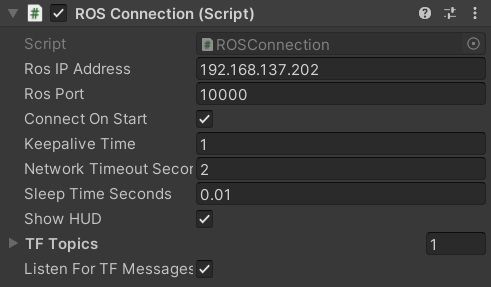
\includegraphics[width=0.5\linewidth]{figs/connection_inspector.png}
        \caption{Unity Connection Inspector}
        \label{fig:unity_connection}
    \end{figure}
    
    % \begin{figure}[htbp]
    %     \centering
    %     \includegraphics[width=\linewidth]{tcp_ip_connection_launch.jpg}
    %     \caption{TCP/IP ROS Node Connection Setup}
    %     \label{fig:tcp_ip_connection}
    % \end{figure}
    \begin{verbatim}
            <arg name="tcp_ip" default="192.168.137.202"/>
            <arg name="tcp_port" default="10000"/>
            
            <node name="server_endpoint" pkg="ros_tcp_endpoint" 
                type="default_server_endpoint.py" args="--wait" output="screen" 
                respawn="true">
                <param name="tcp_ip" type="string" value="$(arg tcp_ip)"/>
                <param name="tcp_port" type="int" value="$(arg tcp_port)"/>
            </node>
    \end{verbatim}
    
    
    This setup is fundamental for the Unity environment to interact effectively with ROS, allowing for real-time data exchange and control commands to be sent between the two systems. Further details are available in the Unity Robotics Hub tutorial on \href{https://github.com/Unity-Technologies/Unity-Robotics-Hub/blob/main/tutorials/ros_unity_integration/network.md}{ROS-Unity integration}.

\end{document}
